\documentclass[12pt,a4paper]{report}

\usepackage[
  a4paper,
  left=3.5cm,
  right=2.5cm,
  top=2.5cm,
  bottom=2.5cm
]{geometry}

\usepackage[T1]{fontenc}
\usepackage[utf8]{inputenc}
\usepackage[polish]{babel}
\usepackage{float}

\usepackage{graphicx}
\graphicspath{{figures/}}
\usepackage[backend=biber,style=numeric,sorting=none]{biblatex}
\addbibresource{bibliography.bib}

\begin{document}

% -----------------------
% Strona tytułowa
% -----------------------
\begin{titlepage}
  \centering
  {\Large\bfseries Uniwersytet Jagielloński w Krakowie\par}
  \vspace{0.5cm}
  {\large Wydział Fizyki, Astronomii i Informatyki Stosowanej\par}

  \vspace{4cm}

  {\Large Kamil Kuziora\par}
  \vspace{0.2cm}
  Nr albumu: 1186631\par

  \vspace{1.5cm}
  {\huge\bfseries System efektów gitarowych w standardzie LV2 do
    przetwarzania sygnału w czasie rzeczywistym z mobilnym interfejsem
  użytkownika\par}
  \vspace{1cm}
  {\large Praca magisterska\par}
  {\large Na kierunku: Informatyka Stosowana\par}

  \vfill

  \begin{flushright}
    \begin{minipage}{0.45\textwidth}
      Praca wykonana pod kierunkiem\\
      \textbf{Dr Hab. Tomasza Urbańczyka}\\
      Wydział Fizyki, Astronomii i Informatyki Stosowanej
    \end{minipage}
  \end{flushright}

  \vfill

  {\large Kraków, \the\year\par}
\end{titlepage}

\newpage

% -----------------------
% Strona z oświadczeniami
% -----------------------
{\noindent\Large\bfseries Oświadczenie kierującego pracą\par}
\vspace{0.8cm}

\indent Potwierdzam, że niniejsza praca została przygotowana pod moim
kierunkiem i kwalifikuje się do przedstawienia jej w postępowaniu o
nadanie tytułu zawodowego.

\vspace{2cm}
\noindent Data \hfill Podpis kierującego pracą\hspace*{1cm} % hspace

\vspace{3cm}

{\noindent\Large\bfseries Oświadczenie autora (autorów) pracy\par}
\vspace{0.8cm}

\indent Świadom odpowiedzialności prawnej oświadczam, że niniejsza
praca dyplomowa została napisana przeze mnie samodzielnie i nie
zawiera treści uzyskanych w sposób niezgodny z obowiązującymi przepisami.

Oświadczam również, że przedstawiona praca nie była wcześniej
przedmiotem procedur związanych z uzyskaniem tytułu zawodowego w
wyższej uczelni.

Oświadczam ponadto, że niniejsza wersja pracy jest identyczna z
załączoną wersją elektroniczną.

\vspace{2cm}
\noindent Data \hfill Podpis autora pracy\hspace*{1cm}

\newpage

\tableofcontents
\newpage

\chapter*{Wprowadzenie}
Rozwój technologii cyfrowych w znaczącym stopniu wpłynął na sposoby
kreowania brzmienia gitary elektrycznej, stopniowo powodując
zastępowanie fizycznych urządzeń ich cyfrowymi odpowiednikami.
Niniejsza praca skupia się na omówieniu autorskiego systemu do
zarządzania cyfrowymi efektami gitarowymi, który został
zaprojektowany specjalnie z myślą o minikomputerach jednopłytkowych
pozbawionych własnego ekranu, takich jak Raspberry Pi. Głównym celem
tego systemu było stworzenie kompletnego rozwiązania dla gitarzystów,
które jest jednocześnie proste w obsłudze, wydajne i przede wszystkim
praktyczne w kreowaniu końcowego brzmienia instrumentu.

Dalsza część pracy krok po kroku wprowadza w techniczne i praktyczne
aspekty projektu. W pierwszej kolejności omówiono pojęcia teoretyczne
niezbędne do pełnego zrozumienia działania systemu. Następnie
przeanalizowano jego architekturę oraz mechanizmy komunikacji między
poszczególnymi komponentami. W kolejnych rozdziałach przybliżono
szczegóły implementacyjne wraz z uzasadnieniem wyboru konkretnych
technologii. Zwieńczeniem pracy jest opis wstępnej konfiguracji
środowiska oraz prezentacja rzeczywistych scenariuszy użycia
stworzonego oprogramowania.

\chapter{Wprowadzenie teoretyczne}
\section{Działanie gitary elektrycznej}
Widoczna na Rysunku \ref{fig:guitar} gitara elektryczna pod względem
konstrukcji znacząco różni się od gitar akustycznych oraz
klasycznych. Ze względu na brak pudła rezonansowego, instrument ten
nie potrafi samodzielnie wzmocnić drgań, ograniczając się jedynie do
cichego wybrzmiewania szarpanych strun.

\begin{figure}[htbp]
  \centering
  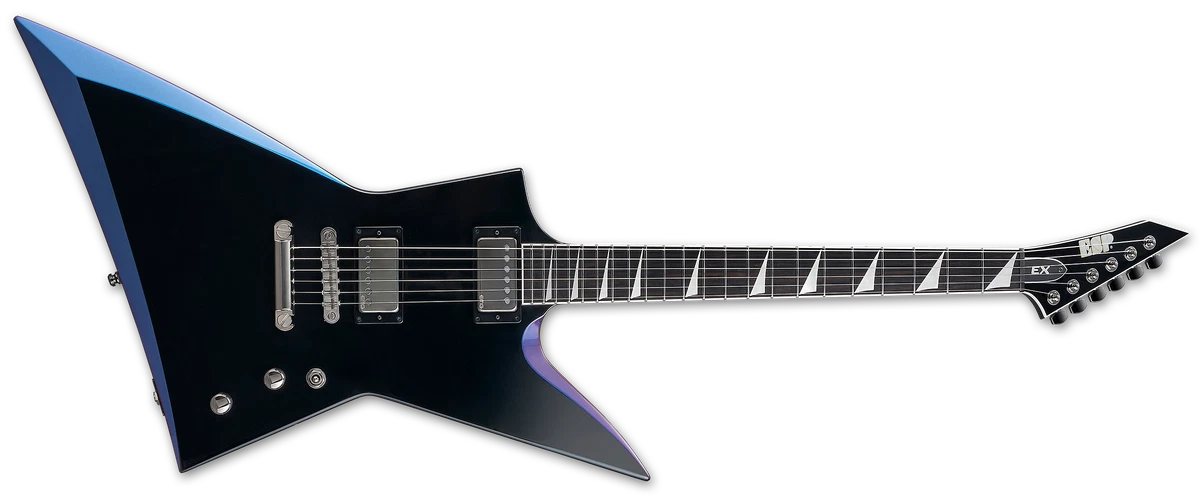
\includegraphics[width=0.8\textwidth]{electric_guitar.png}
  \caption{Gitara elektryczna marki ESP\cite{electric_guitar}}
  \label{fig:guitar}
\end{figure}

Cechą charakterystyczną gitary elektrycznej jest generowanie sygnału
elektrycznego, który musi zostać poddany wzmocnieniu i przetworzeniu,
aby za pośrednictwem głośnika ulec konwersji na słyszalną falę akustyczną.

Sygnał elektryczny w gitarze powstaje dzięki wykorzystaniu
przetworników i opiera się na zjawisku indukcji elektromagnetycznej.
Przetwornik składa się z jednego lub kilku magnesów otoczonych cewką
nawiniętą z cienkiego, miedzianego drutu, co tworzy stałe pole
magnetyczne tuż pod strunami. Kiedy stalowa (ferromagnetyczna) struna
zostaje wprawiona w drgania, jej ruch zaburza to pole magnetyczne. Te
zmiany indukują w cewce napięcie, co powoduje powstanie słabego
sygnału elektrycznego, którego częstotliwość i amplituda wiernie
odzwierciedlają fizyczny ruch
struny\cite{guitar_physics}\cite{guitar_pickup}. Sygnał ten następnie
jest doprowadzany za pomocą kabla (lub rozwiązań bezprzewodowych) do
wzmacniacza lub interfejsu audio.

\section{Sposoby nagłośnienia}
Surowy sygnał pochodzący prosto z gitary elektrycznej jest za słaby,
aby móc samodzielnie wybrzmieć na kolumnach głośnikowych. Do tego
potrzebne jest zastosowanie wcześniej wspomnianego wzmacniacza, który
jest urządzeniem, które w klasycznej postaci składa się z 3
podstawowych komponentów: przedwzmacniacza, końcówki mocy i kolumny
głośnikowej\cite{roland_guitar_amp}. Urządzenie to widoczne jest na
Rysunku \ref{fig:amp}.
\begin{figure}[htbp]
  \centering
  \begin{minipage}{0.48\textwidth}
    \centering
    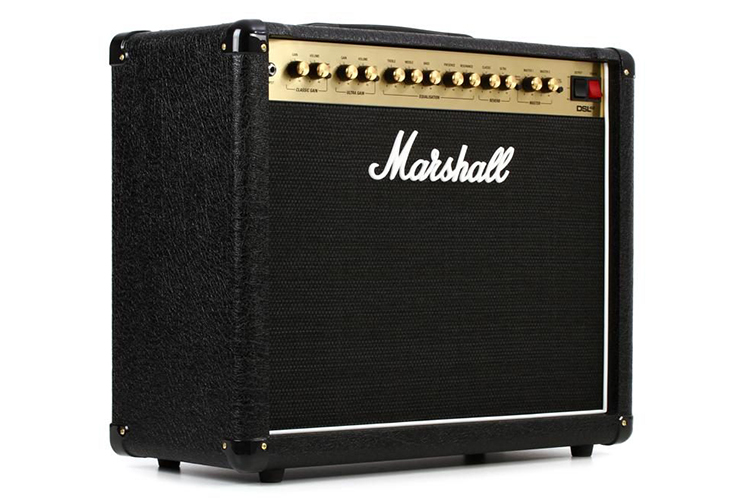
\includegraphics[width=\textwidth]{amp.jpg}
    \caption{Wzmacniacz gitarowy typu \textit{combo}\cite{amp}}
    \label{fig:amp}
  \end{minipage}
  \hfill
  \begin{minipage}{0.48\textwidth}
    \centering
    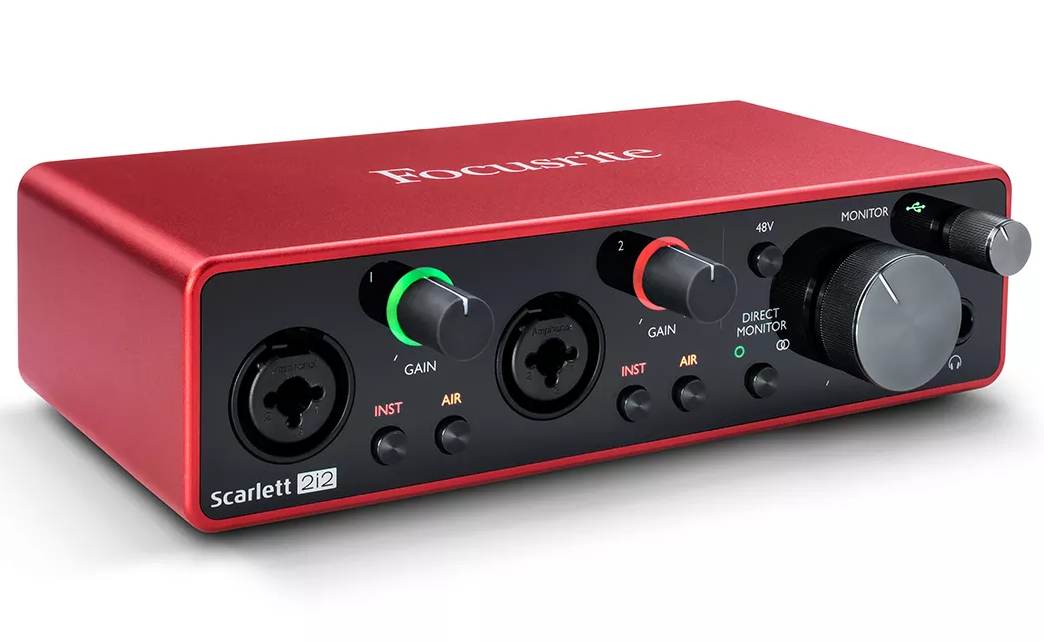
\includegraphics[width=\textwidth]{audio_interface.png}
    \caption{Interfejs audio\cite{audio_interface}}
    \label{fig:audio_interface}
  \end{minipage}
\end{figure}

Każdy z wymienionych wcześniej komponentów ma swoje własne zadanie.
Przedwzmacniacz odbiera słaby sygnał, filtruje sygnał, regulując przy
tym niskie, średnie i wysokie tony, a także kształtuje główny
charakter brzmienia. Kolejnym komponentem na drodze sygnału jest
końcówka mocy, która przyjmuje sygnał charakteryzujący się
odpowiednią barwą i napięciem, ale nie ma wystarczającej mocy do
poruszenia membranami. Rozwiązaniem tego właśnie problemu zajmuje się
ten komponent. Może mieć również wpływ na końcowe brzmienie, co jest
szczególnie widoczne w konstrukcjach lampowych. Finalną częścią są
głośniki, których głównym zadaniem jest zamiana sygnału elektrycznego
na fale akustyczne.

Alternatywne podejście w nagłośnianiu gitary elektrycznej zakłada
użycie interfejsu audio widocznego na Rysunku
\ref{fig:audio_interface} i konwersję sygnału do postaci cyfrowej. To
podejście zostanie w pełni opisane w dalszej części tego dokumentu.

\section{Efekty gitarowe}
Sygnał uzyskany za pomocą opisanych dotychczas komponentów często
okazuje się niewystarczający do realizacji określonych założeń
artystycznych. Poszczególne gatunki muzyczne wymagają odmiennej
charakterystyki barwowej, a sami instrumentaliści dążą do wykreowania
własnego, unikalnego brzmienia. Odpowiedzią na tę potrzebę
różnorodności jest zastosowanie efektów gitarowych.

Klasyczny, sprzętowy efekt gitarowy to z reguły niewielkie urządzenie
elektroniczne, którego głównym elementem jest analogowy lub cyfrowy
układ przetwarzający. Zewnętrzny interfejs urządzenia składa się z
gniazd wejściowych i wyjściowych oraz zestawu potencjometrów i
przełączników, służących do konfiguracji parametrów jego
pracy\cite{effect_unit_wikipedia}.
Pojedyncze efekty są najczęściej łączone szeregowo, tworząc w ten
sposób rozbudowany łańcuch przetwarzania sygnału, który z ang.
powszechnie jest określany jako \textit{pedalboard} (Rysunek
\ref{fig:pedal_board}).

\begin{figure}[htbp]
  \centering
  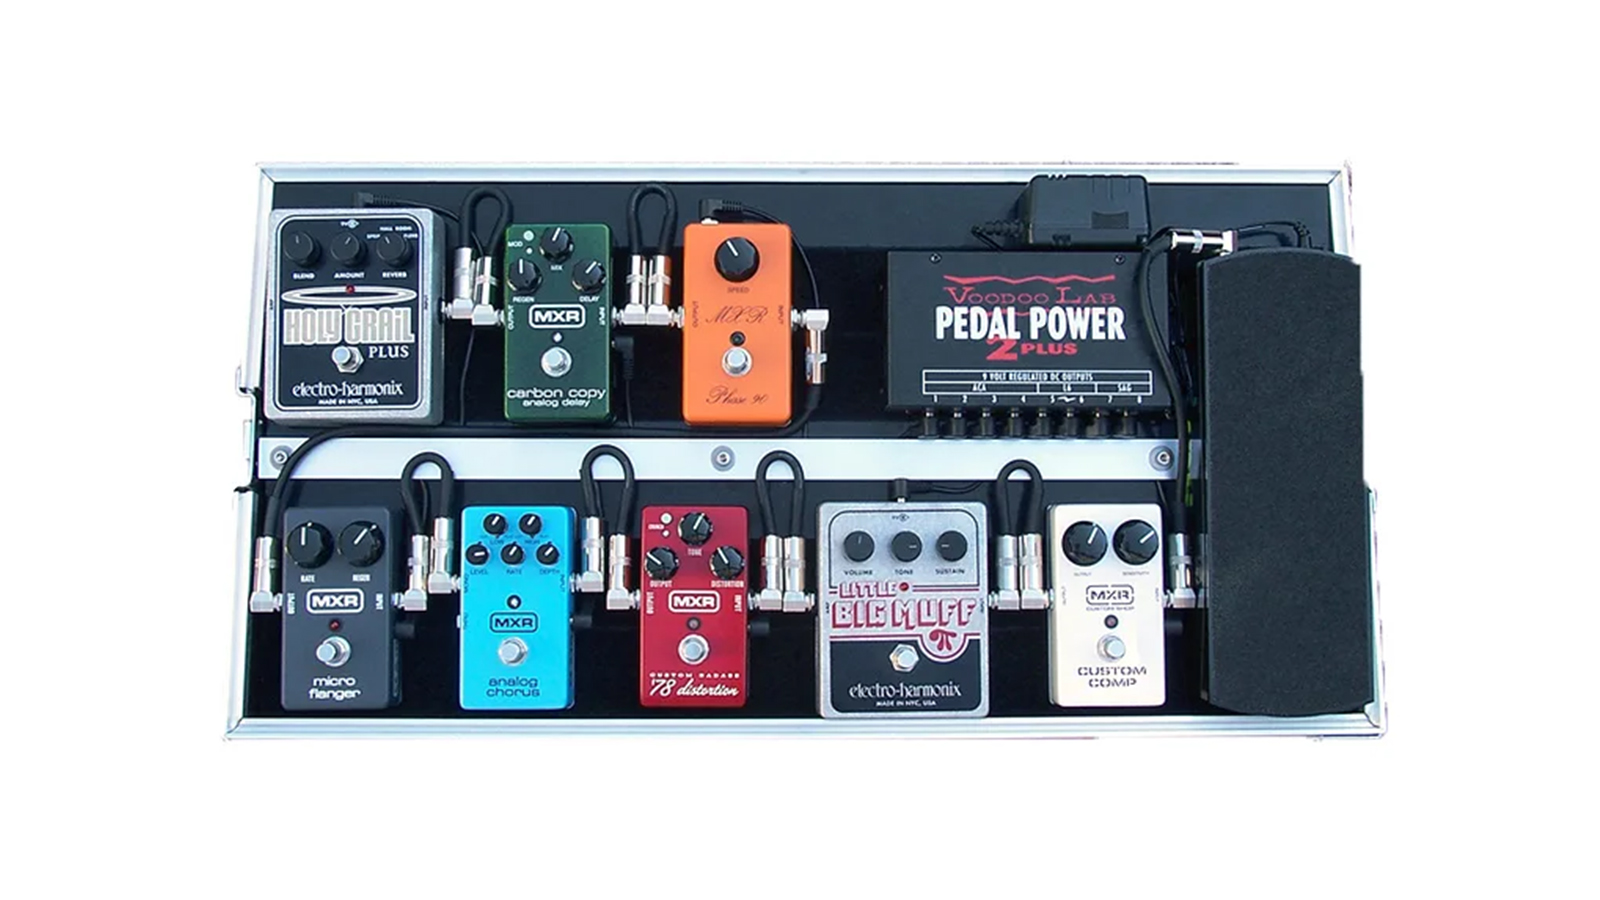
\includegraphics[width=0.8\textwidth]{pedal_board.jpg}
  \caption{Przykładowy \textit{pedalboard}\cite{pedalboard}}
  \label{fig:pedal_board}
\end{figure}
\subsection{Rodzaje efektów gitarowych}
Wyróżnia się kilka głównych kategorii efektów
gitarowych\cite{guitar_peadl_types}:

\begin{enumerate}
  \item \textbf{Przestery} (ang. \textit{Distortion}) -- jedna z
    najpopularniejszych kategorii efektów gitarowych. Ich działanie
    polega na znacznym wzmocnieniu sygnału do poziomu, przy którym
    układ przestaje być w stanie przetworzyć go w sposób liniowy.
    Prowadzi to do obcinania szczytów sygnału, określanego w języku
    angielskim jako \textit{clipping}. Proces ten wprowadza dodatkowe
    składowe harmoniczne, zmieniając brzmienie sygnału w
    charakterystyczny sposób. Przestery gitarowe są szczególnie
    charakterystyczne dla takich gatunków muzycznych jak rock i metal
    \cite{distortion}.
  \item \textbf{Efekty modulacyjne}
    \begin{enumerate}
      \item \textit{Chorus} -- efekt, który przyjmuje sygnał
        wejściowy, a następnie miksuje go z jedną lub kilkoma kopiami
        tego sygnału opóźnionymi w czasie\cite{chorus}.
      \item \textit{Tremolo} -- efekt polegający na okresowej zmianie
        amplitudy sygnału\cite{realization_of_guitar_audio_effects},
        co przekłada się na jego regularne
        ściszanie i pogłaśnianie.
      \item \textit{Phaser} -- efekt, w którym sygnał jest
        rozdzielany na osobne ścieżki. Jedna z nich pozostaje
        niezmieniona, podczas gdy druga przechodzi przez serię
        filtrów powodujących przesunięcia fazowe zależne od
        częstotliwości. W wyniku interferencji obu sygnałów powstają
        okresowe wzmocnienia i osłabienia wybranych zakresów
        częstotliwości, co nadaje brzmieniu charakterystyczny,
        \textit{wirujący} i \textit{przestrzenny} charakter\cite{phaser}.
    \end{enumerate}
  \item \textbf{Efekty przestrzenne i czasowe}
    \begin{enumerate}
      \item \textit{Delay} -- zapisuje sygnał w buforze i odtwarza go
        po określonym czasie, często stosuje się również sprzężenie
        zwrotne, które powoduje serię coraz cichszych powtórzeń.
        Działa podobnie do echa\cite{realization_of_guitar_audio_effects}
      \item \textit{Reverb} -- również opiera się na opóźnionych
        kopiach sygnału, ale jest znacznie bardziej zaawansowany niż
        \textit{deleay}. Pozwala na symulowanie wybrzmiewania dźwięku
        w różnych zamkniętych pomieszczeniach\cite{reverb}.
    \end{enumerate}
  \item \textbf{Efekty filtrujące i modyfikujące częstotliwość}
    \begin{enumerate}
      \item \textit{Korektor barwy (EQ)} -- pozwala na uwidocznienie
        lub wycięcie konkretnych pasm częstotliwości
      \item \textit{Pitch shifter} -- przesuwa cały sygnał o zadany
        interwał muzyczny w górę lub w dół (np. pozwala osiągnąć
        dźwięk o oktawę niższy)
    \end{enumerate}
  \item \textbf{Efekty dynamiczne}
    \begin{enumerate}
      \item \textit{Kompresor} -- zmniejsza rozpiętość dynamiczną
        przez ściszanie najgłośniejszych dźwięków i podbijanie
        cichszych\cite{compressor}, co powoduje wyrównanie dźwięku i wydłużenie
        wybrzmiewania struny (z ang. \textit{sustain})
      \item \textit{Bramka szumów} -- odcina sygnał wejściowy, gdy ten
        spada poniżej ustalonego progu\cite{noise_gate}. Skuteczny w redukcji
        niepożądanych szumów i dźwięków w momencie, gdy muzyk nie gra
        na instrumencie
    \end{enumerate}
\end{enumerate}

\section{Cyfrowe odpowiedniki efektów gitarowych}
Cyfrowym odpowiednikiem efektów gitarowych są wtyczki
audio\cite{audio_effects}, które są programami komputerowymi, które
otrzymują na wejściu sygnał dźwiękowy w postaci cyfrowej,
przetwarzają go, a następnie wysyłają go na wyjście. Podobnie jak
ich fizyczne odpowiedniki, wtyczki audio pozwalają na modyfikowanie
parametrów, z jakimi przetwarzany jest dźwięk.

Wtyczki audio do poprawnego działania wymagają dostarczenia im jednego
lub więcej kanałów wejściowych i wyjściowych, przez które
mogą przepływać próbki dźwiękowe o rozmiarze wspieranym przez daną
wtyczkę. Dodatkowo część wtyczek udostępnia zintegrowany interfejs
użytkownika, który służy do kontrolowania działania wtyczki. Z racji
na charakter efektów gitarowych jako części składowych łańcucha
efektów, a nie samodzielnego bytu, wtyczki potrzebują zewnętrznego
programu do zarządzania nimi.

\subsection{Zarządzanie wtyczkami audio}
Środowiskiem uruchomieniowym dla wtyczek audio jest aplikacja
nadrzędna, określana mianem programu-hosta. Pełni ona pełną kontrolę
nad cyklem życia wtyczki: od jej wyszukania i załadowania do pamięci,
aż po inicjalizację. Sam proces inicjalizacji polega na przekazaniu
wtyczce niezbędnych parametrów środowiskowych, takich jak rozmiar
bufora i częstotliwość próbkowania, oraz dostarczeniu wskaźników do
wejściowych i wyjściowych buforów audio. Ponadto zaawansowany host
odpowiada za routing sygnału - umożliwia łączenie wielu wtyczek w
szeregowy łańcuch przetwarzania oraz swobodną modyfikację ich
kolejności. Oprogramowanie to często zajmuje się również
renderowaniem interfejsów graficznych wtyczek (GUI) oraz pozwala
użytkownikowi na zarządzanie całkowitymi opóźnieniami systemu poprzez
zmianę rozmiaru bufora. Współpraca programów hostujących z
niezależnymi wtyczkami jest możliwa dzięki zastosowaniu
ujednoliconych standardów API, które ściśle definiują protokół
komunikacji pomiędzy obydwoma komponentami.

\subsection{Standardy wtyczek audio}
Współczesny rynek oprogramowania muzycznego charakteryzuje się
mnogością formatów wtyczek audio\cite{plugins_standards}. Najbardziej
rozpowszechnionym z
nich jest VST (ang. Virtual Studio Technology), opracowany przez
niemiecką firmę \textit{Steinberg Media
Technologies}\cite{wikipedia_vst}. Choć format
ten uznawany jest za niekwestionowany standard branżowy, jest to
rozwiązanie własnościowe. Konkurencyjnym, lecz zamkniętym na jeden
ekosystem standardem jest Audio Units (AU) firmy Apple, przeznaczony
wyłącznie dla systemów macOS oraz iOS. Z punktu widzenia urządzeń,
takich jak Raspberry Pi, oraz środowisk opartych na jądrze Linux,
kluczowe znaczenie mają jednak otwarte alternatywy (open-source).
Należą do nich historyczny format LADSPA, jego nowoczesny następca
LV2, a także zyskujący na popularności format CLAP.

\subsection{Standard LV2}
Standard LV2\cite{lv2_website}\cite{lv2_wikipedia} (LADSPA Version 2)
stanowi ewolucyjne rozwinięcie historycznego już interfejsu LADSPA
(ang. \textit{Linux Audio Developer's Simple Plugin API}). Jest to
wieloplatformowy i w pełni otwarty standard wtyczek audio, którego
architekturę oparto na mechanizmie rozszerzeń (ang.
\textit{extensions}). Takie podejście pozwala programistom na
elastyczne implementowanie nowych, zaawansowanych funkcjonalności.
Rozszerzenia, które zyskają aprobatę społeczności i okażą się
uniwersalnie użyteczne, mogą zostać oficjalnie włączone do rdzennej
specyfikacji standardu.

Kluczową zaletą formatu LV2 jest ścisłe odseparowanie warstwy
cyfrowego przetwarzania sygnału (DSP) od interfejsu użytkownika
(GUI). Taki podział nie tylko pozytywnie wpływa na wydajność
obliczeniową, ale przede wszystkim umożliwia zdalne sterowanie
parametrami wtyczek. Z punktu widzenia projektowanego systemu jest to
cecha fundamentalna. Zgodnie z założeniami specyfikacji, wtyczki mogą
opcjonalnie dostarczać własny interfejs graficzny dla
programów-hostów, jednak nie jest to warunek konieczny do ich funkcjonowania.

Kolejnym wyróżnikiem LV2 jest przeniesienie metadanych opisujących
wtyczkę do zewnętrznych plików tekstowych w formacie \textit{Turtle}
(TTL). Pliki te, wykorzystujące struktury danych oparte na trójkach
standardu RDF\cite{rdf}, w sposób precyzyjny i ustandaryzowany
opisują architekturę wtyczki. Definiują one między innymi wszystkie
porty wejściowe i wyjściowe, dostępne parametry (wraz z ich typami i
dopuszczalnymi zakresami wartości), a także informacje
kategoryzacyjne, takie jak klasa wtyczki, nazwa oraz dane autora.
Zastosowanie semantycznego standardu RDF wymusza ścisłe reguły
zapisu, co gwarantuje spójność i maszynową czytelność metadanych
przez programy hostujące.

Zestawienie tych cech – otwartej architektury, izolacji logiki od
interfejsu oraz ustandaryzowanego opisu parametrów – czyni LV2
formatem wyjątkowo atrakcyjnym dla systemów wbudowanych (tzw.
\textit{headless}). Format ten idealnie sprawdza się w rozwiązaniach,
w których warstwa prezentacji została wydzielona do niezależnej
aplikacji (np. mobilnej), komunikującej się z silnikiem audio za
pośrednictwem sieci lokalnej lub protokołu Bluetooth.

\chapter{Przetwarzanie sygnału dźwiękowego w czasie rzeczywistym}

\section{Od sygnału analogowego do domeny cyfrowej}

Gitara elektryczna generuje sygnał, który jest sygnałem ciągłym. Aby
urządzenie cyfrowego mogło poddać go analizie, sygnał ten musi zostać
przetłumaczony na postać dyskretną (cyfrową). Urządzeniem
odpowiedzialnym za ten proces jest interfejs audio ukazany na Rysunku
\ref{fig:audio_interface}, którego kluczowym komponentem jest
przetwornik analogowo-cyfrowy ADC (z ang. \textit{Analog-to-Digital
Converter}). Całą drogę sygnału obrazuje Rysunek \ref{fig:audio_path}

\begin{figure}[htbp]
  \centering
  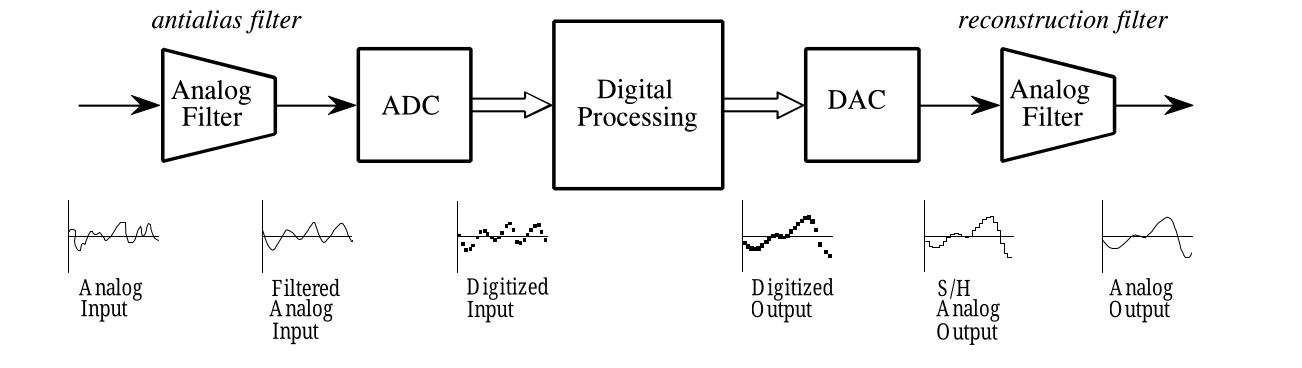
\includegraphics[width=0.95\textwidth]{audio_path.png}
  \caption{Droga sygnału w przetwarzaniu cyfrowym\cite{guide_to_dsp}}
  \label{fig:audio_path}
\end{figure}

W przypadku gitary elektrycznej, zanim sygnał trafi do filtra i
przetwornika ADC, musi przejść jeszcze przez sprzętowy
przedwzmacniacz instrumentalny. Wynika to z faktu, że sygnał
pochodzący z gitary jest słaby.

\subsection{Próbkowanie w czasie (\textit{sampling})}
\textit{Sampling} jest kluczowym procesem w konwersji sygnału z
postaci analogowej do cyfrowej. Polega na cyklicznym pobieraniu i
zapisywaniu chwilowych wartości napięcia sygnału analogowego w ściśle
określonych, równych odstępach czasowych. Istotnym parametrem jest
tutaj częstotliwość próbkowania (z ang. \textit{Sampling Rate}),
który jest wyrażany w $Hz$ i określa, ile takich próbek jest
pobranych w trakcie jednej sekundy.

Aby cyfrowa reprezentacja sygnału była wierna i umożliwiała jego
idealne odtworzenie, częstotliwość próbkowania systemu $f_s$ zgodnie
z twierdzeniem \textit{Nyquista-Shannona} musi spełniać poniższy
warunek \ref{eq:nyquist}.

\begin{equation}
  f_s \geq 2f_{\max}
  \label{eq:nyquist}
\end{equation}

$f_{\max}$ odnosi się w powyższym wzorze do maksymalnej wartości
częstotliwości próbkowanego sygnału. Warto na tym etapie wprowadzić
również pojęcie częstotliwości Nyquista $f_N$, która będzie górną
granicą akceptowanych częstotliwości:

\begin{equation}
  f_N = \frac{f_s}{2}
  \label{eq:nyquist_freq}
\end{equation}

Gdy ta reguła nie jest spełniona, dochodzi do zjawiska określanego
jako \textit{aliasing}. Można je zdefiniować jako krytyczny błąd
dyskretyzacji, prowadzący do nieodwracalnej utraty integralności
widma częstotliwościowego sygnału. Zjawisko to mocno uwidacznia się
na wykresie z Rysunku \ref{fig:aliasing} - widoczna ciągła linia
odpowiada sygnałowi w postaci analogowej, a punkty oznaczają moment w
czasie, gdzie została pobrana próbka. Pobrane wartości nijak mają się
do prawdziwego przebiegu sygnału.

Górna granica słyszanych przez człowieka dźwięków kończy się
przeważnie w okolicy $20kHz$. Z tego też powodu dla prawidłowej
reprezentacji dźwięku powinniśmy wykorzystywać częstotliwość
próbkowania powyżej $40kHz$, co wynika ze wzoru \ref{eq:nyquist}. W
praktyce najczęściej w cyfrowym przetwarzaniu dźwięku wykorzystujemy
częstotliwość $48kHz$.

\begin{figure}[htbp]
  \centering
  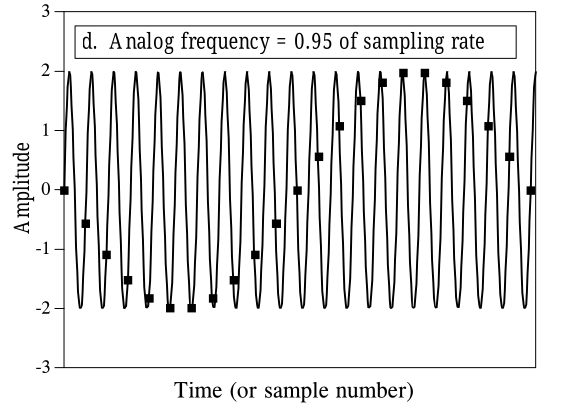
\includegraphics[width=0.8\textwidth]{aliasing.png}
  \caption{Przykład \textit{aliasingu}\cite{guide_to_dsp}}
  \label{fig:aliasing}
\end{figure}

\subsection{Kwantyzacja}
Kolejnym krokiem jest proces kwantyzacji, którego zadaniem jest
zamienienie wartości pobranej próbki (która w praktyce może
przyjmować nieskończenie wiele wartości) do najbliższego dostępnego
poziomu ustalonej, cyfrowej skali. Dokładność tej skali jest
zdefiniowana przez głębię bitową (ang. \textit{Bit Depth}). W
nowoczesnych interfejsach wartość ta zazwyczaj wynosi
24\cite{bit_depth}. Oznacza to w praktyce, że każda próbka może
zostać opisana jedną z $2^{24}$ unikalnych, całkowitych wartości.
Większość nowoczesnych środowisk do przetwarzania dźwięku decyduje
się jednak na konwersję całkowitych wartości zwracanych przez
interfejs na 32-bitowe liczby zmiennoprzecinkowe.

\subsection{Rekonstrukcja sygnału: Konwersja cyfrowo-analogowa}
Gdy urządzenie cyfrowe zakończy przetwarzanie sygnału w postaci
cyfrowej, aby sygnał ten mógł wybrzmieć na membranach głośników,
musimy ponownie przekonwertować go do postaci analogowej.
Przetwornik DAC (\textit{Digital-to-Analog-Converter}), otrzymując
konkretną wartość próbki, generuje odpowiadający jej poziom napięcia
elektrycznego. Następna próbka jednak przyjdzie dopiero za ułamek
milisekundy (wynikający z częstotliwości próbkowania), więc układ
utrzymuje to napięcie do pojawienia się kolejnej próbki. Mechanizm
ten określany jest z ang. jako \textit{Zero-Order Hold} i produkuje
sygnał, który ma postać schodkową widoczną na Rysunku \ref{fig:zoh}.

\begin{figure}[htbp]
  \centering
  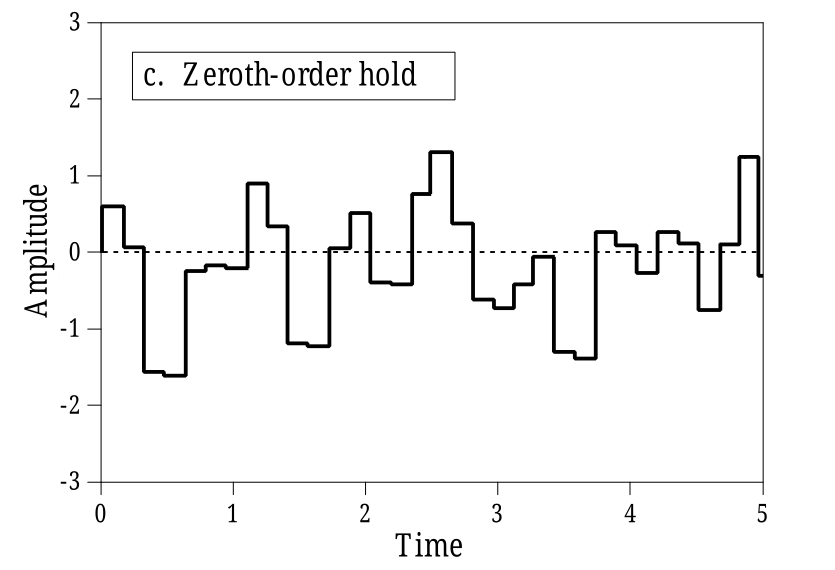
\includegraphics[width=0.8\textwidth]{zoh.png}
  \caption{Działanie Zero-Order Hold\cite{guide_to_dsp}}
  \label{fig:zoh}
\end{figure}

Taka postać sygnału zawiera wiele wysokoczęstotliwościowych
składowych, które są powyżej częstotliwości $f_N$. Aby je
usunąć, stosuje się filtr analogowy, który określany jest mianem
filtra rekonstrukcyjnego, który stara się wyciąć wszystkie niechciane
składowe. Otrzymany w ten sposób sygnał może już trafić np. do
wzmacniacza wyjściowego, skąd może trafić do przetworników elektroakustycznych.

\section{Cyfrowe przetwarzanie dźwięku (DSP)}
Gdy sygnał dźwiękowy opuszcza ADC, przyjmuje postać ciągłego
strumienia dyskretnych wartości liczbowych. Teoretycznie system
mógłby przyjmować, przetwarzać i odsyłać każdą próbkę z osobna
natychmiast po jej zarejestrowaniu. W przypadku systemów operacyjnych
ogólnego przeznaczenia, takie podejście byłoby skrajnie nieefektywne.
Wymagałoby to od procesora przełączania kontekstu (ang.
\textit{context switching}) $48000$ razy na sekundę (zakładając
\textit{sampling rate} na poziomie $48kHz$), co znacząco
ograniczyłoby jego możliwości wykonywania innych zadań np.
przetwarzania samego dźwięku.

Rozwiązaniem tego problemu jest wprowadzenie mechanizmu buforowania.
System kolekcjonuje próbki z dźwiękiem i w momencie, gdy zostanie
osiągnięta ich określona ilość, następuje przerwanie, które informuje
o gotowości danych do dalszego przetwarzania. Ta ilość próbek jest
istotnym parametrem i jest określana jako rozmiar bufora (z ang.
\textit{buffer size}).

\subsection{Opóźnienia}
Wprowadzenie mechanizmu buforowania jest konieczne, ale wiąże się z
pewnymi opóźnieniami. Pomijając opóźnienia w działaniu interfejsu
audio i transportu danych za pomocą USB, czas potrzebny na
uzupełnienie bufora $t_b$ wynosi:

\begin{equation}
  t_b = \frac{n}{f_{s}}
  \label{eq:buffer_time}
\end{equation}

\noindent Gdzie $f_s$ to częstotliwość próbkowania, a $n$ to rozmiar bufora.

Ze wzoru \ref{eq:buffer_time} wynika, że dla częstotliwości
próbkowania $f_s$ równej 48 kHz oraz bufora o rozmiarze $n = 128$
próbek, czas niezbędny na zgromadzenie danych wynosi $t_b \approx$
2,67 ms. System dysponuje dokładnie takim samym przedziałem czasu na
przetworzenie pełnego bloku danych przez algorytmy DSP, a następnie
zapisanie wyniku do bufora wyjściowego (w tym samym czasie układ
sprzętowy gromadzi już w tle próbki dla kolejnego cyklu). Wynika z
tego, że teoretyczne, minimalne opóźnienie wprowadzane przez
architekturę oprogramowania wynosi $2t_b$. Wartość ta stanowi jednak
wyłącznie dolną granicę, ponieważ uwzględnia jedynie czas sprzętowego
kolekcjonowania próbek i ich cyfrowego przetwarzania, pomijając
narzuty wynikające z pozostałych elementów systemu.

Z perspektywy muzyka kluczowym parametrem jest opóźnienie całkowite
(ang. \textit{Round-Trip Latency}, RTL), definiowane jako czas, który
upływa od momentu fizycznego wyzwolenia dźwięku (np. szarpnięcia
struny) do chwili usłyszenia przetworzonego sygnału akustycznego. Na
całkowitą wartość RTL składają się następujące czynniki:

\begin{enumerate}
  \item czas konwersji w układach ADC i DAC,
  \item latencja transmisji danych (np. pakietyzacja na magistrali USB),
  \item narzut systemu operacyjnego (w tym opóźnienia planisty, ang.
    \textit{scheduling latency}),
  \item wspomniany wcześniej czas pracy z buforami,
  \item latencja akustyczna, wynikająca z czasu propagacji fali
    dźwiękowej w powietrzu (w przypadku korzystania z wolnostojących głośników).
\end{enumerate}

Sumaryczny narzut wprowadzany przez układy konwersji oraz
dwukierunkową transmisję USB może wahać się w przedziale od 1,5 ms do
3,8 ms\cite{audio_intetface_overhead}. Ponadto propagacja dźwięku w
powietrzu generuje opóźnienie rzędu 2,9 ms na każdy metr odległości
od źródła. Przyjmując częstotliwość próbkowania 48 kHz, rozmiar
bufora równy 128 próbek oraz wykorzystanie interfejsu audio średniej
klasy w połączeniu ze słuchawkami (co pozwala na eliminację latencji
akustycznej), wypadkowe opóźnienie całkowite powinno wynosić w
przybliżeniu 7,5 ms.

Tolerancja na opóźnienia jest kwestią subiektywną i zależy w dużej
mierze od charakterystyki wykorzystywanego instrumentu. W praktyce
szacuje się, że wartości RTL poniżej 6–8 ms zapewniają pełny komfort
gry i są niemal niedostrzegalne dla wykonawcy. Z kolei opóźnienia
rzędu 14–16 ms stają się już odczuwalne, jednak wciąż pozwalają na
swobodną grę na instrumencie\cite{perception_of_latency}

\section{Stos przetwarzania dźwięku systemu GNU/Linux}

Linuksowy stos audio ma budowę warstwową: dostęp do sprzętu,
zarządzanie grafem połączeń oraz właściwe przetwarzanie sygnału są
rozdzielone między osobne komponenty. Ta modularność oraz otwartość
jądra sprawiają, że Linux jest chętnie wybierany do budowy
dedykowanych urządzeń audio na komputerach jednopłytkowych klasy Raspberry Pi.

\subsection{ALSA}

Bezpośredni dostęp do interfejsu audio zapewnia podsystem ALSA
(\textit{Advanced Linux Sound Architecture}), działający na poziomie
jądra. Odpowiada on za sterowniki sprzętowe i bufory DMA, a serwery
wyższego poziomu, w tym JACK, korzystają z niego zamiast komunikować
się ze sprzętem bezpośrednio \cite{gentoo_jack}.

\subsection{JACK}

Ponad ALSA działa JACK Audio Connection Kit - serwer przestrzeni
użytkownika pośredniczący między aplikacjami-klientami a sprzętem.
JACK to demon serwera audio, który umożliwia klientom przetwarzanie i
routing danych audio oraz MIDI w sposób synchroniczny, dokładny co do
próbki i o niskim opóźnieniu \cite{jackd_manpage}, przy czym klienci
mogą działać jako osobne procesy lub jako klienci wewnętrzni
uruchamiani w ramach procesu serwera \cite{jackd_manpage}. Każdy
klient udostępnia porty, które JACK organizuje w graf połączeń. Gdy
uruchamiany jest program obsługujący JACK, jego wejścia i wyjścia
stają się widoczne dla innych programów obsługujących JACK, dzięki
czemu można je łączyć w dowolny sposób
\cite{libremusicproduction_jack}, a serwer może pełnić rolę
nadrzędnego zegara synchronizującego wszystkich klientów. Dane
pomiędzy klientami krążą w postaci 32 bitowych, zmiennoprzecinkowych próbek.

\subsection{Model callback}
\label{sec:jack_callback}

Sercem architektury JACK jest cykliczne przetwarzanie oparte na
funkcjach zwrotnych (ang. \textit{callback}). Serwer działa w wątku
czasu rzeczywistego, który w stałych odstępach (period) aktywuje
kolejno wszystkich klientów w grafie. Każdy klient rejestruje własną
funkcję przetwarzającą, wywoływaną raz na cykl: odbiera bufor próbek
wejściowych, przetwarza go i zwraca bufor wyjściowy przed upływem
przydzielonego czasu. Synchroniczne wykonanie wszystkich callbacków w
danym cyklu, zgodnie z topologią grafu, gwarantuje deterministyczny
przepływ danych od wejścia, przez kolejne aplikacje przetwarzające,
aż po wyjście audio.

\section{Programowanie czasu rzeczywistego}
Jak wspomniano wcześniej, oprogramowanie przetwarzające sygnał w
reżimie czasu rzeczywistego dysponuje ściśle określonym oknem
czasowym na wykonanie wszystkich operacji obliczeniowych dla danego
bufora. Niedotrzymanie tego terminu i opóźnienie w dostarczeniu
przetworzonej ramki danych skutkuje przerwaniem ciągłości strumienia
audio. Zjawisko to objawia się wystąpieniem słyszalnych zniekształceń
i artefaktów, takich jak trzaski (ang. \textit{glitch} lub
\textit{audio dropout}) na urządzeniach wyjściowych\cite{real_time_101}.

Duże ograniczenia czasowe dla programów przetwarzających dźwięk
oznaczają poświęcenie większej uwagi, jakie operacje są wykonywane w
funkcji, która bezpośrednio zajmuje się przetwarzaniem otrzymanych
buforów. Aplikacje pracujące z dźwiękiem to prawie zawsze aplikacje
wielowątkowe. Z tego też powodu niejednokrotnie wątek zajmujący się
przetwarzaniem dźwięku musi dzielić stan z drugim wątkiem np.
odpowiedzialnym za rysowanie interfejsu użytkownika, który służy do
kontroli parametrów, z jakimi przetwarzany jest sygnał. W klasycznych
programach, naturalnym podejściem byłoby zastosowanie mechanizmów
synchronizacji, takich jak \textit{mutex}. W przypadku programowania
czasu rzeczywistego wszystkie blokady nie wchodzą w rachubę. Zamiast
mechanizmów synchronizacji powinno się zastosować nieblokujące metody
synchronizacji jak np. komunikacja za pośrednictwem buforów cyklicznych.

Oczywistą operacją w trakcie zwykłego programowania jest również
alokowanie pamięci lub jej zwalnianie. Tymczasem systemowe operacje
zarządzania stertą są z natury niedeterministyczne. Mogą one wymagać
długotrwałego przeszukiwania wolnych bloków pamięci, oczekiwania na
zwolnienie blokad współdzielonych z wolniejszymi wątkami aplikacji, a
także wywoływać kosztowne narzuty związane z tzw. błędami braku
strony (ang. \textit{page fault}) w pamięci wirtualnej. Nawet
pojedyncze opóźnienie wynikające z tych mechanizmów prowadzi do
niedotrzymania terminu przetwarzania i przerwania ciągłości sygnału
audio. Z tego względu cała pamięć niezbędna do działania algorytmów
DSP musi zostać prealokowana podczas początkowej fazy inicjalizacji,
jeszcze przed uruchomieniem głównej pętli przetwarzającej dźwięk.

Ze względu na rygorystyczne ograniczenia czasowe, w głównym wątku
czasu rzeczywistego niedopuszczalne jest wykonywanie jakichkolwiek
operacji wejścia/wyjścia (ang. \textit{Input/Output}, I/O).
Restrykcja ta dotyczy operacji na systemie plików (odczyt i zapis
dyskowy), interakcji ze standardowymi strumieniami systemowymi (np.
wypisywania informacji do konsoli), a także komunikacji sieciowej z
wykorzystaniem gniazd (ang. \textit{sockets}). Z perspektywy wąskiego
okna czasowego, operacje te są niezwykle kosztowne, a co
najważniejsze – skrajnie niedeterministyczne. Próba ich wykonania
grozi wstrzymaniem działania wątku audio (ang. \textit{thread
blocking}) i przerwaniem ciągłości dźwięku.

\chapter{Architektura projektu}
W niniejszym rozdziale zaprezentowano architekturę oraz szczegóły
techniczne zrealizowanego systemu do zarządzania cyfrowymi efektami
gitarowymi. Stanowi on płynne przejście od rozważań teoretycznych
dotyczących cyfrowego sygnału i wymogów środowiska czasu
rzeczywistego, do praktycznej implementacji omawianych zagadnień. W
kolejnych sekcjach szczegółowo omówiono zagadnienia architektoniczne,
obejmujące podział systemu na komponenty i sposoby komunikacji między
tymi komponentami. Przybliżono również model wielowątkowy komponentu
czasu rzeczywistego, a także wyjaśniono metody synchronizacji stanu z
wątkiem czasu rzeczywistego.

\section{Środowisko uruchomieniowe}
System został zaprojektowany do uruchamiania na urządzeniach
jednopłytkowych takich jak Raspberry Pi. Urządzenia te, w większości
przypadków są oparte o procesor w architekturze ARM, ale sam system
jest również wspierany na architekturze x86. Nacisk projektu na
wykorzystanie tego typu urządzeń wynika głównie z ich niewielkiego
rozmiaru i znikomego zapotrzebowania na energię. Działanie całego
systemu zostało oparte o system operacyjny GNU/Linux, a dokładniej
dystrybucję Debian. Wybór tej konkretnej dystrybucji został w dużej
mierze podyktowany dużą stabilnością i oficjalnymi zaleceniami
producentów Raspberry Pi 5, na którym testowany był system. Użyte
technologie do stworzenia systemu są wymienione w dalszej części dokumentu.

\section{Składowe systemu}

System ma architekturę modularną, składającą się z 3 kluczowych
komponentów widocznych na rysunku \ref{fig:general_architecture}.

\begin{figure}[htbp]
  \centering
  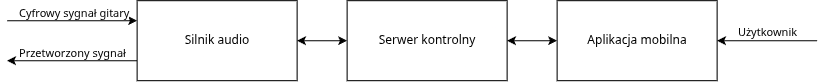
\includegraphics[width=1.0\textwidth]{general_architecture.drawio.png}
  \caption{Podział systemu na składowe [źródło własne]}
  \label{fig:general_architecture}
\end{figure}

\subsection{Silnik audio}
Główny komponent, którego zadaniem jest praca z wtyczkami i
przetwarzanie dźwięku za ich pomocą. Umożliwia wyszukiwanie,
ładowanie z dysku, wstępną inicjalizację, organizację, ustawianie
parametrów wtyczek, a także zajmuje się dostarczaniem odpowiednich
wejść i wyjść dla tych wtyczek. Do jego obowiązków należy również
zarejestrowanie w systemie klienta JACK, a także wszystkich
wymaganych portów. Silnik odpowiedzialny jest również za zarządzanie
wirtualnym grafem połączeń dźwiękowych, a także kontrolą parametrów z
jakimi przetwarzany jest dźwięk (\textit{buffer size} i
\textit{sampling rate}). Komponent ten udostępnia API, oparte o
gniazda, które umożliwia wysyłanie poleceń umożliwiających np.
pobranie aktualnego stanu lub wykonanie konkretnej operacji.

\subsection{Serwer kontrolny}
Głównym zadaniem serwera kontrolnego jest pośredniczenie w
komunikacji pomiędzy silnikiem audio, aplikacją mobilną, a także bazą
danych. Komponent ten w reakcji na zapytania płynące z aplikacji
mobilnej, przetwarza je, generuje odpowiednią wiadomość, a następnie
wysyła ją za pomocą gniazd do silnika audio i oczekuje na odpowiedź
po czym przekierowuje ją z powrotem do aplikacji mobilnej.
Udostępnia REST API, a także zajmuje się obsługą połączeń z
wykorzystaniem \textit{web sockets} z pomocą, których rozsyła
powiadomienia o zdarzeniach zgłaszanych przez silnik audio do
wszystkich podłączonych instancji aplikacji mobilnych. Razem z
silnikiem audio, pracują pod kontrolą jednego urządzenia.

\subsection{Aplikacja mobilna}
Aplikacja na urządzenia mobilne jest głównym interfejsem dla
użytkownika, który pozwala mu kontrolować zachowanie systemu. Z
poziomu aplikacji, użytkownik może obserwować aktualny stan łańcucha
efektów gitarowych i wykonywać na nim wszelkie operacje. Posiada
również możliwość kontrolowania ustawień, z jakimi działa system -
może zarządzać aktywnymi urządzeniami wejścia i wyjścia, a także
sterować opóźnieniami przez modyfikację rozmiaru bufora. Aplikacja
komunikuje się bezpośrednio z serwerem kontrolnym za pomocą
dostępnego REST API i połączenia z wykorzystaniem \textit{web sockets}.

\subsection{Zalety architektury modularnej}
Kluczowa zaleta podziału systemu na niezależny silnik audio oraz
serwer sterujący pozwala na odseparowanie krytycznego czasowo
przetwarzania dźwięku od operacji związanych z komunikacją sieciową,
obsługą aplikacji oraz dostępem do bazy danych. Dzięki temu silnik
audio może koncentrować się na realizacji przetwarzania sygnału w
czasie rzeczywistym, podczas gdy serwer sterujący pełni funkcję
warstwy pośredniczącej odpowiedzialnej za koordynację komunikacji
pomiędzy poszczególnymi komponentami systemu.

Dodatkową zaletą takiego podziału jest elastyczność systemu oraz
możliwość jego dalszej rozbudowy. Umieszczenie logiki sterującej w
niezależnym serwerze pozwala na oddzielenie sposobu komunikacji z
użytkownikiem od samego silnika przetwarzania dźwięku. W rezultacie w
przyszłości możliwe byłoby dodanie kolejnych interfejsów sterowania,
takich jak komunikacja Bluetooth, gRPC, interfejs wiersza poleceń czy
nawet dedykowany fizyczny kontroler wyposażony w pokrętła i
przyciski, bez konieczności modyfikowania logiki odpowiedzialnej za
przetwarzanie sygnału audio.

Nowy interfejs musiałby jedynie komunikować się z warstwą
odpowiedzialną za sterowanie systemem i korzystać z istniejącego
mechanizmu zarządzania stanem oraz komunikacji z silnikiem audio.
Dzięki temu poszczególne sposoby sterowania mogą być rozwijane
niezależnie od siebie, a architektura systemu pozostaje otwarta na
przyszłe rozszerzenia. Takie podejście ogranicza również zależność
systemu od konkretnej technologii komunikacyjnej oraz konkretnego
rodzaju interfejsu użytkownika.

\section{Schemat komunikacji}
Podział systemu na trzy odrębne komponenty architektoniczne wiąże się
ze znacznymi wyzwaniami komunikacyjnymi. Z jednej strony aplikacja
kliencka musi mieć zapewniony natychmiastowy dostęp do aktualnego
stanu silnika audio, z drugiej zaś – dysponować możliwością
dynamicznego wpływania na jego pracę. O ile operacje takie jak
dodawanie nowych wtyczek czy zmiana globalnych ustawień
konfiguracyjnych można z powodzeniem realizować za pośrednictwem
klasycznego wzorca REST API, problematyczna staje się płynna
regulacja parametrów w czasie rzeczywistym. Interakcja użytkownika z
kontrolką interfejsu (np. wirtualnym potencjometrem) generuje
dziesiątki zdarzeń w ułamku sekundy. W takim scenariuszu każdorazowe
wysyłanie żądania z użyciem protokołu HTTP wprowadzałoby
nieakceptowalny narzut sieciowy oraz zauważalne opóźnienia.

Kolejnym kluczowym wyzwaniem jest utrzymanie ścisłej spójności
pomiędzy stanem prezentowanym w aplikacji mobilnej a faktycznym
stanem silnika audio. Sytuację dodatkowo komplikuje wymóg obsługi
wielu klientów jednocześnie – użytkownik może bowiem sterować
systemem równolegle z poziomu kilku urządzeń (np. smartfonu i
tabletu). Wymusza to zaprojektowanie mechanizmu natychmiastowej
propagacji zmian i synchronizacji interfejsów na wszystkich
podłączonych urządzeniach.

\subsection{Podział operacji}
Kluczowym założeniem architektonicznym przy projektowaniu komunikacji
pomiędzy komponentami systemu było zdefiniowanie dwóch kategorii
przepływu danych: operacji kosztownych oraz operacji lekkich.
Operacje kosztowne dotyczą zmian stanu lub zapytań, które wymagają
komunikatu zwrotnego bądź potwierdzenia wykonania zadania przez
silnik audio. Działania te charakteryzują się stosunkowo niską
częstotliwością występowania. Typowym przykładem takiej operacji jest
proces dodawanie nowej wtyczki lub żądanie pobrania pełnego stanu
systemu – sekwencja ta wymaga wysłania zapytania, przetworzenia go
przez silnik, a następnie oczekiwania na odpowiedź.

Przeciwieństwo stanowią operacje lekkie, realizowane w modelu
jednokierunkowym (często określanym jako \textit{fire-and-forget}),
które z założenia nie wymagają bezpośredniego potwierdzenia odbioru
od adresata. Z reguły są one wykonywane z bardzo dużą
częstotliwością. Do tej grupy zalicza się wspomnianą wcześniej,
płynną regulację parametrów wtyczek oraz asynchroniczne rozgłaszanie
zdarzeń (ang. \textit{events}) informujących podłączonych klientów o
aktualizacjach w silniku audio.

\subsection{Komunikacja silnik audio - serwer kontrolny}
\label{sec:communication_engine-server}
Schemat komunikacji pomiędzy silnikiem audio a serwerem kontrolnym
znajduje się na Rysunku \ref{fig:engine-server_communication}.

\begin{figure}[htbp]
  \centering
  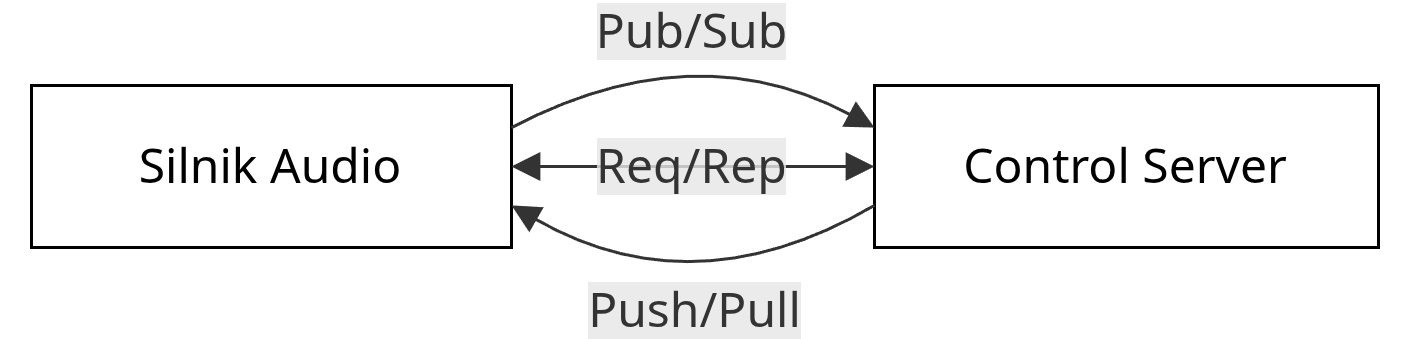
\includegraphics[width=0.8\textwidth]{engine-server_communication.png}
  \caption{Schemat komunikacji silnik audio - serwer kontrolny[źródło własne]}
  \label{fig:engine-server_communication}
\end{figure}

Komunikacja pomiędzy tymi dwoma komponentami odbywa się za pomocą 3
różnych zestawów gniazd dostępnych w bibliotece \textit{ZeroMQ}:
\begin{enumerate}
  \item \textit{REQ/REP} -- są wykorzystywanie głównie do obsługi
    operacji kosztownych, które wymagają odpowiedzi od silnika audio
    np. pobranie aktualnego stanu
  \item \textit{PUSH/PULL} -- gniazda zajmujące się komunikacją typu
    \textit{fire-and-forget}. Wykorzystywane są do obsługi dużej
    ilości poleceń lekkich np. zmiany parametrów wtyczki
  \item \textit{PUB/SUB} -- za pomocą tych gniazd silnik audio wysyła
    powiadomienia o wszystkich zmianach stanu do jednego lub więcej
    subskrybentów. Dla każdego urządzenia, które połączy się z
    serwerem kontrolnym, tworzone jest osobne gniazdo nasłuchujące
\end{enumerate}

Ponieważ założono, że silnik audio oraz serwer kontrolny będą
domyślnie funkcjonować w obrębie tego samego urządzenia sprzętowego,
do wymiany danych między nimi wykorzystano mechanizm gniazd domeny
uniksowej (ang. \textit{Unix Domain Sockets}). Stanowią one wysoce
zoptymalizowaną formę komunikacji międzyprocesowej (ang.
\textit{Inter-Process Communication}, IPC), która omija pełny stos
sieciowy systemu operacyjnego, co znacząco redukuje opóźnienia. Warto
przy tym zaznaczyć, że przyjęta architektura nie wymusza ścisłej
lokalności komponentów. Zastosowana abstrakcja oparta na standardowym
interfejsie gniazd pozwala na łatwą zmianę protokołu (np. na gniazda
TCP/UDP), umożliwiając komunikację przez sieć.

W celu dalszej optymalizacji zastosowano w pełni binarny format
przesyłanych wiadomości. Pozwala to na eliminację kosztownego narzutu
obliczeniowego związanego z parsowaniem i serializacją tekstu
(charakterystycznego dla formatów takich jak JSON czy XML), czyniąc
opóźnienia komunikacyjne niemal znikomymi. Takie podejście gwarantuje
wyjątkowo wysoką wydajność systemu, a równoległe zastosowanie trzech
niezależnych zestawów gniazd znacząco zwiększa jego całkowitą przepustowość.

\subsection{Komunikacja serwer kontrolny - aplikacja mobilna}
Schemat komunikacji pomiędzy serwerem kontrolnym a aplikacją mobilną
znajduje się na Rysunku \ref{fig:server-app_communication}.

\begin{figure}[htbp]
  \centering
  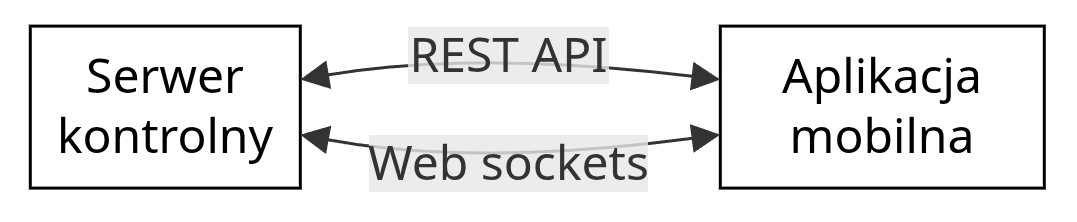
\includegraphics[width=0.8\textwidth]{server-app_communication.png}
  \caption{Schemat komunikacji serwer kontrolny - aplikacja
  mobilna[źródło własne]}
  \label{fig:server-app_communication}
\end{figure}

Zgodnie z przyjętym podziałem, realizacja operacji kosztownych odbywa
się za pośrednictwem interfejsu REST API, natomiast do obsługi
operacji lekkich i częstych wykorzystano protokół WebSocket.
Komunikacja oparta na tej technologii ma charakter w pełni
dwukierunkowy (ang. \textit{full-duplex}). Dzięki temu aplikacja
kliencka może w sposób ciągły wysyłać polecenia sterujące (np.
regulację parametrów), a jednocześnie asynchronicznie odbierać
powiadomienia o zmianach stanu.

Po zestawieniu połączenia sieciowego pomiędzy instancją aplikacji a
serwerem kontrolnym, serwer ten subskrybuje strumień zdarzeń
pochodzących z silnika audio. Pełni on tym samym funkcję aktywnego
pośrednika – nasłuchuje na komunikaty nadchodzące z lokalnych gniazd
IPC, a następnie niezwłocznie propaguje je do podłączonych urządzeń
docelowych. Wymiana informacji na zewnętrznej warstwie sieciowej
(pomiędzy serwerem kontrolnym a aplikacją kliencką) oparta jest na
formacie JSON, który stanowi powszechnie uznany i optymalny standard
dla tego typu komunikacji.

\section{Schemat wielowątkowości silnika audio}
Na Rysunku \ref{fig:engine_arch} zaprezentowany jest schemat
obrazujący działanie silnika audio:

\begin{figure}[h]
  \centering
  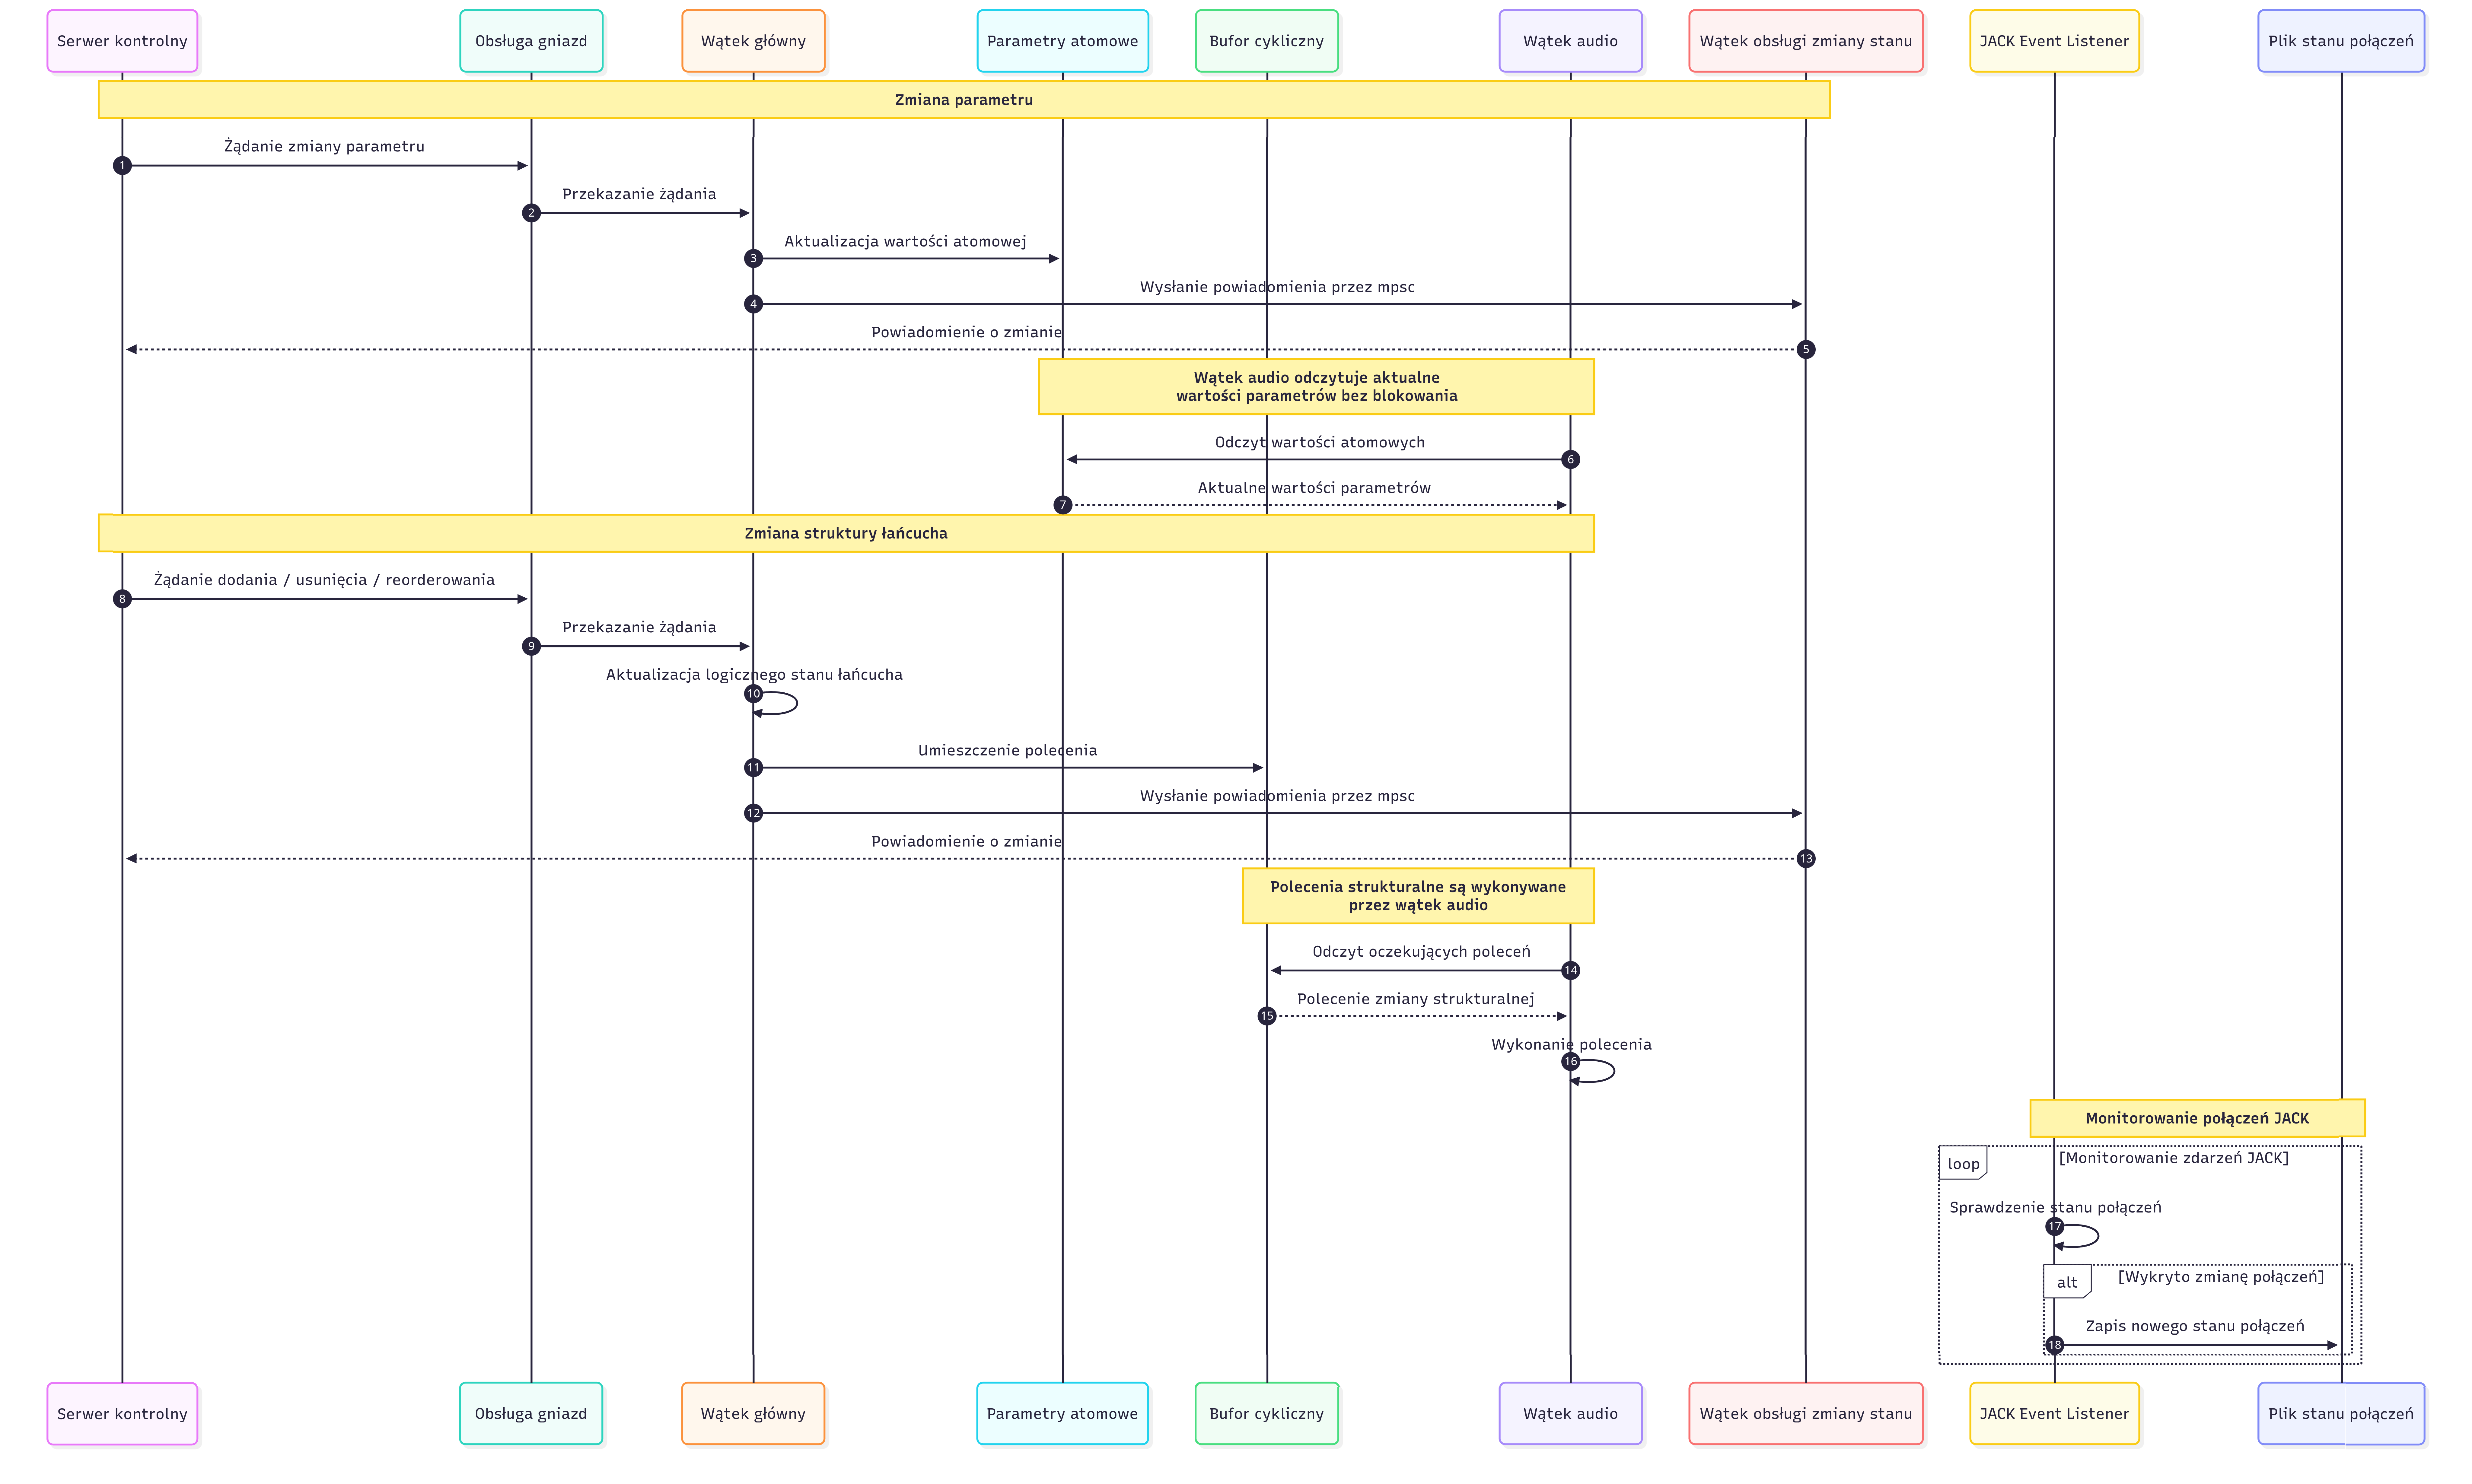
\includegraphics[width=1.0\textwidth]{engine_architecture.png}
  \caption{Architektura silnika audio[źródło własne]}
  \label{fig:engine_arch}
\end{figure}

Kluczowym aspektem architektonicznej strony silnika audio jest
zapewnienie bezkolizyjnej i wysoce wydajnej komunikacji pomiędzy
priorytetowym wątkiem przetwarzającym dźwięk a resztą wątków
silnika. Łączy on wykorzystanie prawdziwych wątków, jak i podejścia
asynchronicznego, które w szczególności pozwala na wygodną obsługę
wielu gniazd jednocześnie.

Fundamentem przetwarzania sygnału jest wspomniany w sekcji
\ref{sec:jack_callback} \textit{callback} serwera JACK, operujący w
dedykowanym, izolowanym wątku czasu rzeczywistego (wątek audio).
Aktualny stan parametrów wszystkich wtyczek przechowywany jest w
głównym wątku silnika w postaci wektora zmiennych atomowych
zmiennoprzecinkowych (ang. \textit{atomic floats}). Zastosowanie
typów atomowych gwarantuje, że wątek audio może w sposób ciągły i
całkowicie nieblokujący odczytywać aktualne wartości z pamięci, unikając blokad.

Szczególnym przypadkiem są operacje strukturalne, takie jak
dodawanie, usuwanie lub zmiana kolejności wtyczek w łańcuchu
sygnałowym. Działania te często wymagają wykonywania operacji
dyskowych, alokacji pamięci na ciężkie struktury lub tworzenia instancji
wtyczek. Wszystkie te operacje są wymagające i wolne, dlatego
wykonywane są na głównym wątku silnika. Gdy zostaną ukończone, główny
wątek przygotowuje polecenie, które następnie jest pakowane do
jednokierunkowego bufora cyklicznego i za jego sprawą trafia do wątka
audio. Ten, na samym początku każdego cyklu przetwarzania (ang.
\textit{sweep}), weryfikuje stan bufora cyklicznego, asymilując nowe
instrukcje przed rozpoczęciem modyfikacji dźwięku, po czym aplikuje
je do swojego wektora aktywnych instancji.

Aby wyeliminować konieczność odpytywania wątku audio o swój stan,
wątek główny silnika posiada ciągle aktualizowany wektor, zapisujący
informacje o aktualnej topologii łańcucha efektów. Takie podejście
sprawia, że wątek główny jest w stanie w każdej chwili, bez
blokowania wątku audio, zwrócić kompletny i aktualny stan, z jakim
pracuje silnik. Dodatkowo, w systemie powołano do życia komponent określany
jako \textit{JACK Event Listener}, którego zadaniem jest
monitorowanie zdarzeń asynchronicznych serwera JACK. Jego głównym
zadaniem jest monitorowanie aktualnych połączeń pomiędzy portami
klienta JACK i zapisywanie wszystkich zmian w pliku JSON, po to aby
po restarcie silnika móc ponownie przywołać stan połączeń dźwiękowych.

Warstwa API, stanowiąca punkt styku z serwerem kontrolnym,
zrealizowana została z wykorzystaniem architektury wielozadaniowej.
Główny proces asynchroniczny odbiera polecenia z gniazd sieciowych,
delegując pracę do odpowiednich metod silnika audio. Równolegle
funkcjonuje obsługa powiadomień, nasłuchująca zmiany stanu silnika
audio przez kanał komunikacyjny typu \textit{Multi-Producer,
Single-Consumer} - MPSC. Po każdej istotnej zmianie w stanie wysyłane
jest powiadomienie do wszystkich subskrybentów za pomocą gniazda \textit{PUB}.

\chapter{Szczegóły implementacyjne}

\section{Wykorzystane technologie}
W niniejszej sekcji omówiono kluczowe technologie oraz narzędzia
programistyczne wykorzystane na etapie implementacji zrealizowanego systemu.

\subsection{Silnik audio}
Silnik audio zaimplementowano w języku \textit{Rust}. Język ten
charakteryzuje się wydajnością obliczeniową porównywalną z językami C
i C++, oferując jednocześnie nowoczesną składnię. Jego fundamentalną
cechą jest wbudowany mechanizm \textit{borrow
checker}\cite{rust_docs}, który już na etapie kompilacji
rygorystycznie weryfikuje bezpieczeństwo dostępu do pamięci. Chociaż
rygor ten niejednokrotnie wydłuża proces pisania kodu, to w końcowym
rozrachunku skutecznie zapobiega trudnym w diagnozie błędom (takim
jak wycieki pamięci czy \textit{race conditions}), co jest aspektem
krytycznym przy budowie systemów czasu rzeczywistego.

Warstwę przetwarzania dźwięku oparto na architekturze serwera JACK
oraz dedykowanej bibliotece klienckiej. Jest to rozwiązanie
stanowiące branżowy standard w profesjonalnych środowiskach
linuksowych, gwarantujące wysoką stabilność oraz pracę z niskimi opóźnieniami.

Obsługa wtyczek realizowana jest za pośrednictwem biblioteki
\textit{Lilv}, a dokładniej jej odpowiednika dla języka
\textit{Rust}. Narzędzie to automatyzuje proces indeksowania
dostępnych w systemie wtyczek w standardzie LV2 oraz dostarcza
przejrzyste API na szereg istotnych operacji (od inicjalizacji po
mapowanie portów wejścia i wyjścia).

Istotnym elementem architektury komunikacyjnej silnika jest również
biblioteka \textit{ZeroMQ}. W sposób znaczący ułatwia ona operowanie
na gniazdach UNIX, oferując wydajne środowisko i różnorodne metody komunikacji.

\subsection{Serwer kontrolny}
Ten komponent systemu również został opracowany przy użyciu języka
\textit{Rust}. Zastosowanie ujednoliconego stosu technologicznego
drastycznie uprościło komunikację pomiędzy silnikiem audio a serwerem
kontrolnym. Pozwoliło to na współdzielenie definicji struktur danych
opisujących przesyłane komunikaty pomiędzy oboma modułami. Dzięki
temu mechanizm binarnego kodowania i dekodowania informacji stał się
w pełni zunifikowany, eliminując konieczność pisania podwójnego kodu
dla różnych środowisk.

Ponadto, użycie jednego języka programowania dla całej warstwy
lokalnej (uruchamianej na urządzeniu) umożliwiło wykorzystanie
wbudowanego w narzędzie \textit{Cargo} mechanizmu przestrzeni
roboczych (ang. \textit{workspaces}). Pozwala to na wygodne dzielenie
wspólnych zależności oraz zintegrowany proces kompilacji wielu
podprojektów jednocześnie.

Do obługi połączeń sieciowych wykorzystano bibliotekę \textit{Axum},
która oferuje również wsparcie dla \textit{web sockets}. W roli bazy
danych wykorzystano \textit{Sqlite}, które jest minimalistycznym i
wydajnym rozwiązaniem. Do komunikacji z bazą danych wykorzystano
bibliotekę \textit{SeaORM}.

\subsection{Aplikacja mobilna}
Do implementacji aplikacji klienckiej wybrano framework \textit{React
Native}. Wybór ten był podyktowany nie tylko obszernym ekosystemem
dostępnych bibliotek, ale przede wszystkim możliwością tworzenia
oprogramowania wieloplatformowego (ang. \textit{cross-platform}).
Pozwoliło to na jednoczesne wsparcie systemów operacyjnych iOS oraz
Android przy wykorzystaniu pojedynczej bazy kodu.

\section{Przegląd implementacyjny silnika audio}
W niniejszej sekcji omówiono szczegóły implementacyjne silnika audio.
Zaprezentowano w niej kluczowe struktury, zdefiniowano ich zakres
odpowiedzialności oraz opisano zachodzące między nimi relacje i
interakcje. W tej sekcji będzie wielokrotnie pojawiać się słowo
\textit{struktura} zamiast \textit{klasa}, ponieważ język
\textit{Rust} nie jest językiem obiektowym (ale wspiera część jego koncepcji).

\subsection{\textit{EngineClient}}

\begin{figure}[h]
  \centering
  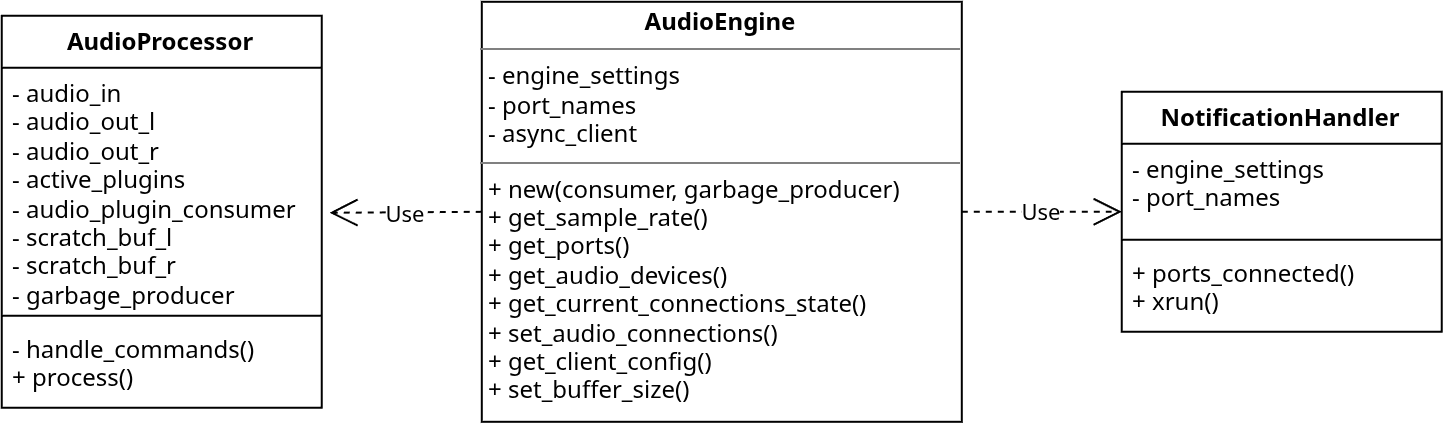
\includegraphics[width=1.0\textwidth]{engine_client_uml.drawio.png}
  \caption{Schemat UML dla \textit{EngineClient}[źródło własne]}
\end{figure}

Struktura \textit{EngineClient} odpowiada bezpośrednio za integrację
systemu z serwerem JACK. Do jej głównych zadań należy inicjalizacja
instancji klienta, rejestracja portów wejściowych i wyjściowych,
zarządzanie topologią połączeń pomiędzy portami audio, a także
automatyczne przywracanie zapisanych wcześniej tras sygnałowych po
restarcie silnika. Ponadto, struktura ta udostępnia API, które
pozwala na odczyt bieżących parametrów środowiska uruchomieniowego
(takich jak częstotliwość próbkowania i rozmiar bufora) oraz
informacji o aktywnych połączeniach, jak również dostarcza metody
umożliwiające ich dynamiczną modyfikację. Dodatkowo rejestruje w
kliencie JACK dwie kluczowe struktury \textit{AudioProcessor} i
\textit{NotificationHandler}.

\subsubsection{AudioProcessor}
Omawiana struktura funkcjonuje w obrębie dedykowanego wątku audio,
przeznaczonego wyłącznie do przetwarzania sygnału w reżimie czasu
rzeczywistego. Jej metoda \textit{process} jest cyklicznie wywoływana
przez serwer JACK w celu operowania na napływających próbkach.
Struktura ta zarządza prywatnym wektorem przechowującym instancje
zainicjalizowanych wtyczek. Algorytmy poszczególnych wtyczek są
aplikowane do bufora wejściowego sekwencyjnie, ściśle według
kolejności ich występowania w wektorze. Kluczowym elementem działania
metody \textit{process} jest faza wstępna - metoda odpytuje bufor
cykliczny. Jeżeli znajdują się w nim zakolejkowane polecenia
strukturalne, są one aplikowane do prywatnego wektora wtyczek.

\subsubsection{NotificationHandler}
Metody omawianej struktury są wywoływane w odpowiedzi na określone
zdarzenia systemowe zgłaszane przez serwer JACK. Procedura
\textit{ports\_connected} aktywowana jest przy każdej zmianie
trasowania sygnału. Weryfikuje ona, czy wykryte zmiany dotyczą portów
należących do klienta aplikacji, a w przypadku potwierdzenia –
utrwala zaktualizowany schemat połączeń w pliku konfiguracyjnym. Ten
sam plik wykorzystywany jest następnie podczas procesu rozruchu
silnika do automatycznego odtworzenia początkowej struktury połączeń.

Z kolei metoda \textit{xrun} wykrywa i loguje przypadki wystąpienia zjawiska
znanego jako \textit{XRUN} - \textit{buffer underrun/overrun}.
Zjawisko to oznacza niedotrzymanie rygorystycznego limitu czasu
przeznaczonego na przetworzenie bieżącej ramki danych audio, co w
konsekwencji prowadzi do przerwania ciągłości sygnału i powstania
słyszalnych zniekształceń lub trzasków (ang. \textit{audio glitch}).

\subsection{\textit{PluginManager}}
\begin{figure}[h]
  \centering
  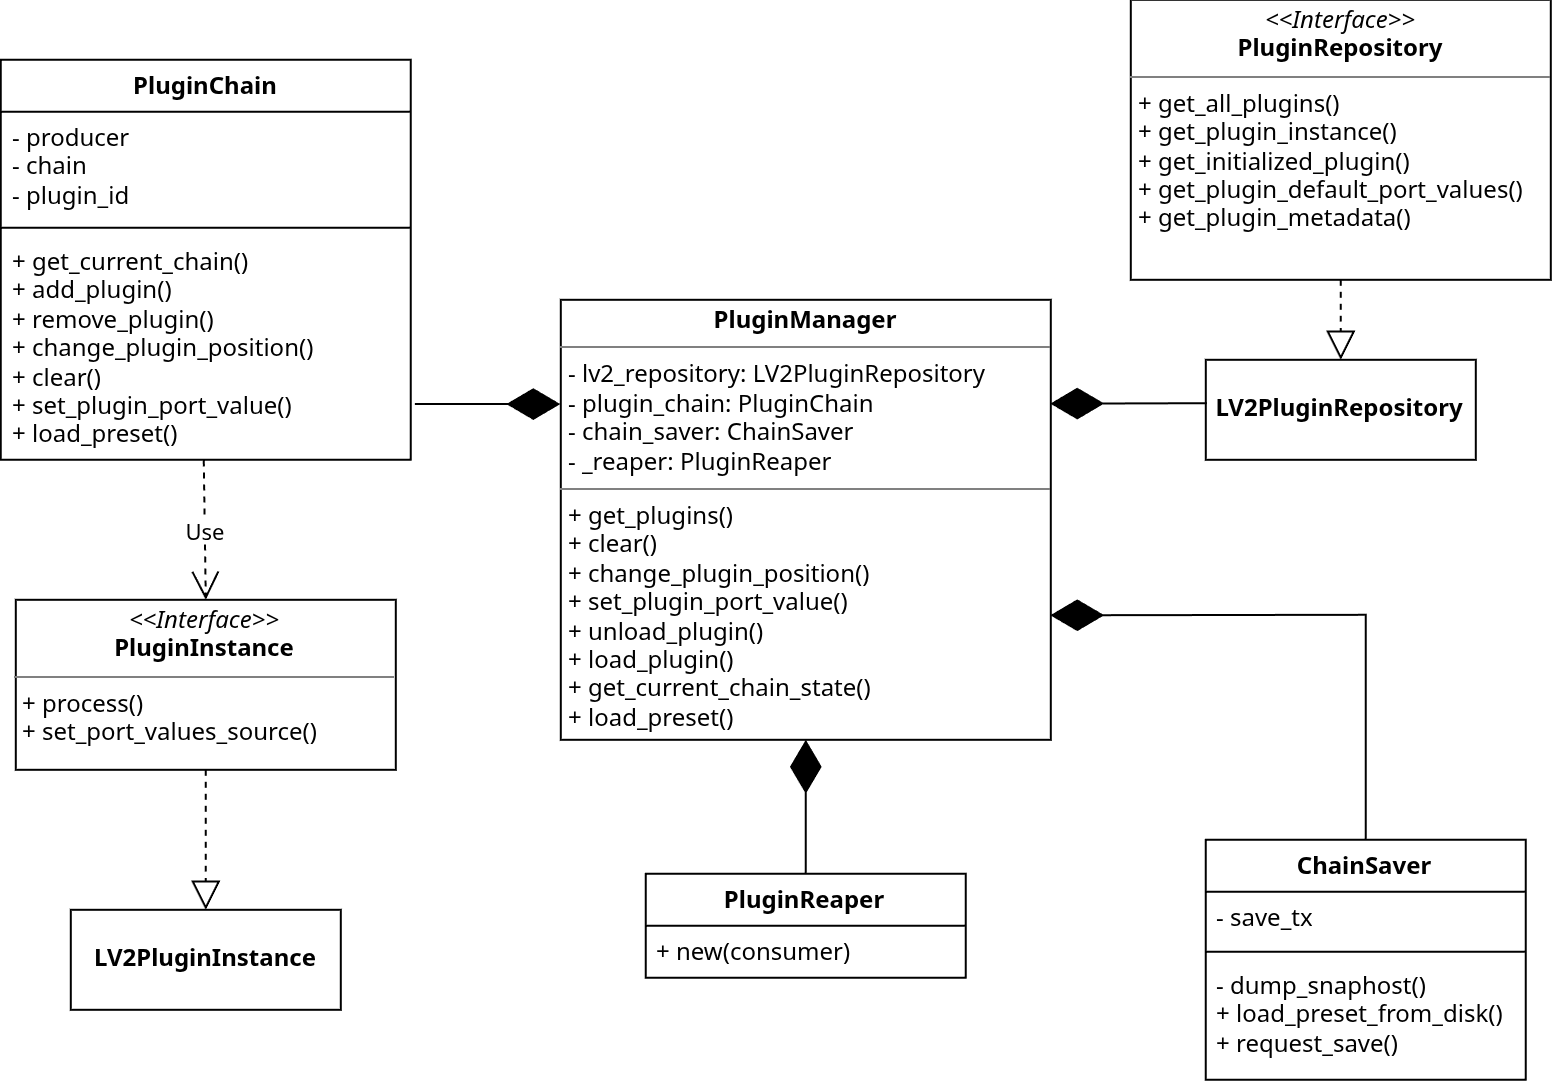
\includegraphics[width=1.0\textwidth]{plugin_manager_uml.drawio.png}
  \caption{Schemat UML dla \textit{PluginManager}[źródło własne]}
\end{figure}

Struktura \textit{PluginManager} odpowiada za realizację wszystkich
operacji związanych z wtyczkami audio – począwszy od zwracania listy
dostępnych wtyczek, poprzez ich inicjalizację i usuwanie, aż po
modyfikację ich parametrów oraz zmianę położenia w wirtualnym
łańcuchu efektów. Z architektonicznego punktu widzenia komponent ten
implementuje wzorzec strukturalny Fasady (ang. \textit{Facade}).
Hermetyzuje on wewnętrzną złożoność systemu, delegując zadania
związane ze wstępnym wyszukiwaniem i zarządzaniem bibliotekami do
komponentu \textit{LV2PluginRepository}, natomiast żądania
modyfikacji samej topologii łańcucha przetwarzania przekazuje do
struktury \textit{PluginChain}. Ponadto omawiana struktura odpowiada
za zapisywanie wszelkich zmian wprowadzanych w łańcuchu wtyczek do
pliku. Plik ten następnie jest używany do przywołania ostatniego
stanu po ponownym uruchomieniu silnika.

\subsubsection{PluginChain}
Przechowuje stan łańcucha wtyczek i udostępnia metody, które
pozwalają go modyfikować. Struktura ta odpowiada również za
informowanie wątku audio o zmianach w łańcuchu poprzez wysyłanie
stosownych wiadomości za pomocą bufora cyklicznego.

\subsubsection{LV2PluginRepository}
Omawiana struktura implementuje cechę (ang. \textit{trait} - w
  środowisku języka Rust stanowiącą odpowiednik klasycznego interfejsu
obiektowego) o nazwie \textit{PluginRepository}. Do jej głównych
zadań należy realizacja wszelkich działań na samych wtyczkach -
wyszukiwanie, listowanie czy ładowanie z dysku i tworzenie instancji.

Choć w obecnej iteracji systemu, gdzie komponent
\textit{PluginManager} bazuje wyłącznie na implementacji
\textit{LV2PluginRepository}, zastosowanie dodatkowej abstrakcji może
wydawać się zabiegiem nadmiarowym, ale jest to w pełni świadoma
decyzja architektoniczna. Stanowi ona fundament pod przyszłą
rozbudowę systemu o obsługę kolejnych formatów wtyczek audio (np.
CLAP). Interfejs \textit{PluginRepository} odegra wówczas kluczową
rolę jako elastyczny kontrakt dla warstwy zarządzającej wtyczkami.

\subsubsection{LV2PluginInstance}
Omawiana struktura implementuje cechę \textit{PluginInstance}.
Stanowi ona warstwę abstrakcji nad API wtyczek w standardzie LV2,
dostarczając zunifikowaną metodę \textit{process}. Metoda ta
przyjmuje wskaźniki do buforów wejściowych i wyjściowych (dla lewego
i prawego kanału audio). Do jej głównych zadań należy przekazanie
owych wskaźników bezpośrednio do wtyczki, aktualizacja wartości na
portach kontrolnych (odpowiadających za bieżące parametry efektu)
oraz wywołanie wewnętrznej procedury cyfrowego przetwarzania sygnału.

Podobnie jak w przypadku warstwy repozytorium, oparcie architektury
na wspólnym interfejsie \textit{PluginInstance} gwarantuje ścisłą
separację logiki specyficznej dla konkretnego standardu wtyczek od
głównego rdzenia silnika audio. Rozwiązanie to hermetyzuje detale
implementacyjne LV2, stanowiąc solidny fundament pod bezinwazyjną
integrację alternatywnych formatów wtyczek w przyszłych iteracjach
rozwoju systemu.

\subsection{ChainSaver}
Pomocnicza struktura odpowiedzialna za udostępnianie metod
ułatwiających zapis i odczyt zapisanego stanu łańcucha efektów.

\subsection{\textit{MessageHandler}}

\begin{figure}[h]
  \centering
  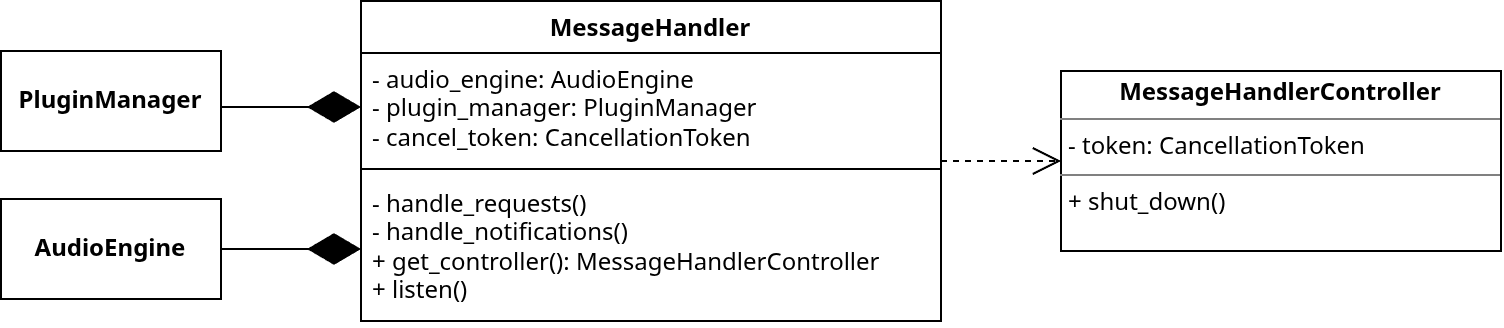
\includegraphics[width=1.0\textwidth]{message_handler_uml.drawio.png}
  \caption{Schemat UML dla \textit{MessageHandler}[źródło własne]}
\end{figure}
Struktura \textit{MessageHandler} odpowiada za udostępnienie
interfejsu API, umożliwiającego zewnętrzne sterowanie silnikiem audio
za pośrednictwem gniazd. Pełni ona funkcję asynchronicznego
kontrolera w odpowiedzi na zdekodowane komunikaty wejściowe, deleguje
wykonanie żądanych operacji do odpowiednich instancji zarządzających,
takich jak \textit{EngineClient} (w przypadku operacji na samym
kliencie JACK) lub \textit{PluginManager} (w przypadku modyfikacji
łańcucha efektów). Obsługa wejścia/wyjścia (I/O) dla gniazd
realizowana jest w sposób w pełni asynchroniczny z wykorzystaniem
środowiska uruchomieniowego \textit{Tokio}. Szczegółowy schemat tej
komunikacji został omówiony w sekcji \ref{sec:communication_engine-server}.

\subsubsection{MessageHandlerController}
Jest to struktura pomocnicza, pełniąca rolę dedykowanego mechanizmu
kontrolnego (zbliżonego koncepcyjnie do wzorca \textit{cancellation
token}). Charakteryzuje się ona możliwością swobodnego klonowania i
bezpiecznego przekazywania pomiędzy różnymi kontekstami wykonawczymi
środowiska asynchronicznego. Jej wyłącznym zadaniem jest umożliwienie
bezpiecznego i kontrolowanego przerwania asynchronicznej pętli
nasłuchującej na przychodzące komunikaty.

\section{Łączenie aplikacji mobilnej z serwerem kontrolnym}

Proces nawiązywania połączenia pomiędzy aplikacją kliencką a serwerem
kontrolnym opiera się na komunikacji sieciowej, co wiąże się z
koniecznością zlokalizowania serwera kontrolnego w sieci lokalnej
(LAN). Aby zautomatyzować ten proces, zaimplementowano mechanizm
wykrywania usług oparty na protokole mDNS (ang. \textit{Multicast
DNS}). Po stronie systemu GNU/Linux (działającego na urządzeniu
docelowym) wykorzystano demona \textit{Avahi}, który rozgłasza w
sieci obecność serwera kontrolnego jako dedykowanej usługi.

Aplikacja mobilna rozpoczyna swoje działanie od przeszukiwania
lokalnej sieci w celu znalezienia usługi o nazwie ściśle
odpowiadającej konfiguracji zdefiniowanej w zmiennych środowiskowych
(jeśli w pamięci jest już zapisany, krok skanowania jest pomijany).
Zastosowanie takiego podejścia znacząco wpływa na prostotę
użytkowania z perspektywy końcowego użytkownika. Pomimo automatyzacji
tej części, użytkownik może manualnie wprowadzić adres lokalnego urządzenia.

Dodatkowo, w scenariuszach, w których podłączenie obu urządzeń do tej
samej zewnętrznej infrastruktury sieciowej jest niemożliwe (np. w
warunkach scenicznych bez routera Wi-Fi), system wspiera połączenie
bezpośrednie. Urządzenie hostujące (np. Raspberry Pi) funkcjonuje
wówczas jako bezprzewodowy punkt dostępowy (ang. \textit{hotspot /
Access Point}). Co istotne, z punktu widzenia warstwy aplikacyjnej
proces odnajdywania serwera i zestawiania połączenia przebiega w tym
trybie identycznie, nie wymagając dodatkowej logiki.

Po pomyślnym zlokalizowaniu serwera kontrolnego i nawiązaniu
połączenia, aplikacja kliencka zapisuje znaleziony adres IP w pamięci
urządzenia. Przy każdym kolejnym uruchomieniu aplikacja w pierwszej
kolejności próbuje połączyć się z zapisanym adresem. Dopiero w
przypadku niepowodzenia, aplikacja ponownie uruchamia pełną procedurę
skanowania sieci za pomocą mDNS. Rozwiązanie to znacząco skraca czas
inicjalizacji aplikacji przy codziennym użytkowaniu.

\section{Przygotowanie urządzenia do pracy z systemem}
W celu znacznego uproszczenia procesu wdrożenia (ang.
\textit{deployment}) systemu na docelowym urządzeniu sprzętowym, w
ramach pracy przygotowano dedykowany skrypt konfiguracyjny,
dostosowany pod dystrybucje GNU/Linux oparte o Debiana. Do jego
obowiązków należy między innymi instalacja wszystkich niezbędnych
zależności, prekonfiguracja demona \textit{Avahi} (w celu poprawnego
rozgłaszania usługi w sieci mDNS), a także pobranie i instalacja
bazowego zestawu wtyczek audio. W ramach tego ostatniego kroku system
wyposażany jest w popularne efekty pochodzące z popularnej aplikacji
\textit{Guitarix}, co zapewnia użytkownikowi dostęp do podstawowej
palety brzmień natychmiast po instalacji.

Działania automatyzujące objęły również fazę działania systemu.
Opracowano odrębny skrypt rozruchowy (ang. \textit{startup script}),
którego zadaniem jest uruchomienie silnika audio i serwera
kontrolnego. Rozwiązanie to całkowicie uwalnia użytkownika od
konieczności ręcznego zarządzania procesami i wpisywania złożonych
poleceń w terminalu.

\chapter{Przykładowe scenariusze użytkowania}
\section{Zarządzanie efektami}
\subsection{Dodawanie wtyczek}
Po pomyślnym zakończeniu procesu nawiązywania połączenia z serwerem
kontrolnym, użytkownikowi prezentowany jest główny interfejs
aplikacji, zilustrowany na rysunku \ref{fig:main_screen_empty}. Ekran
ten w przyszłości posłuży do wizualizacji aktywnego łańcucha efektów.

\begin{figure}[H]
  \centering
  \begin{minipage}[t]{0.45\textwidth}
    \centering
    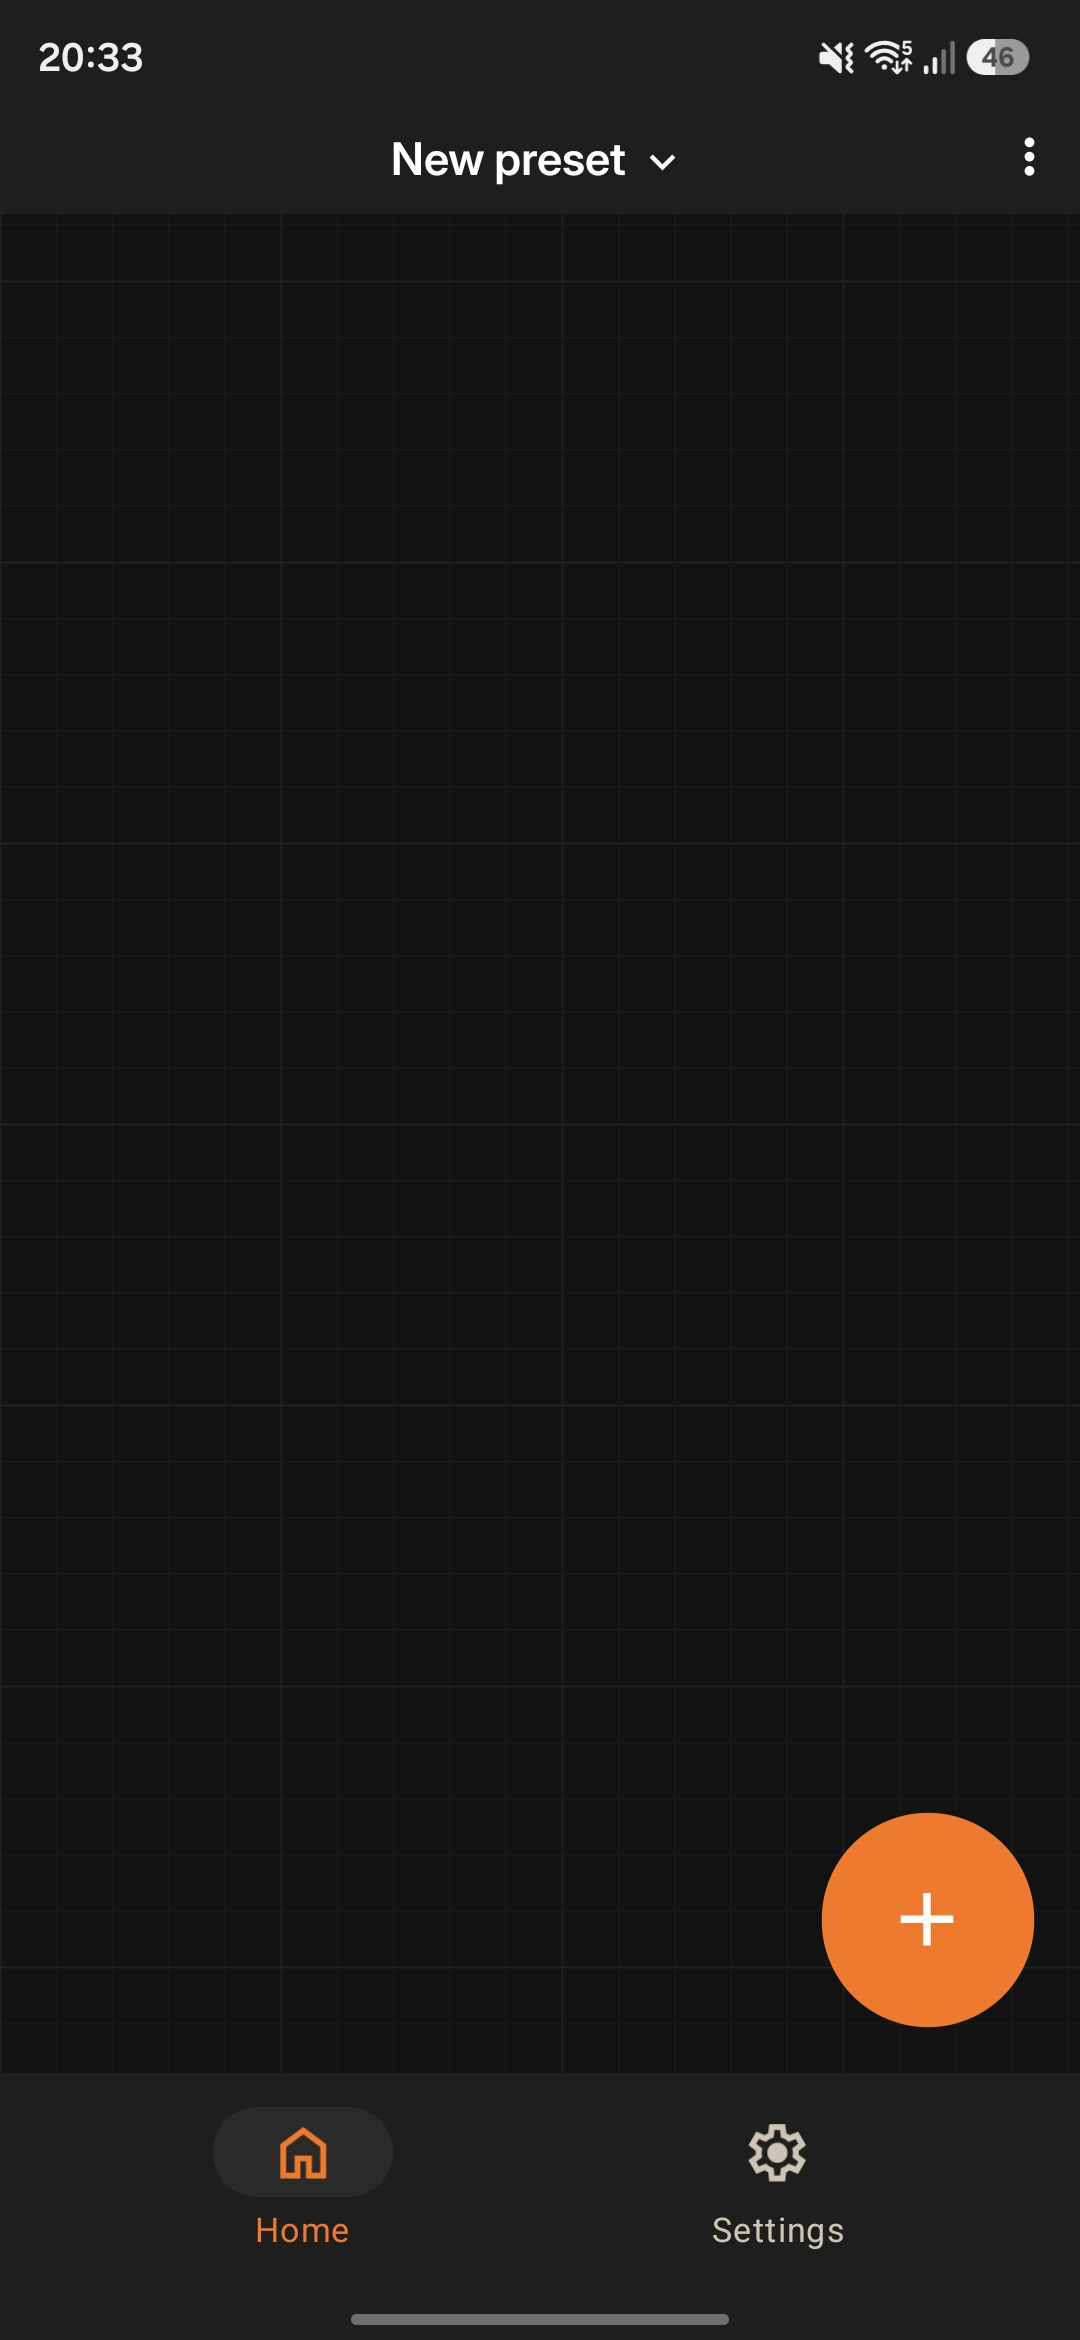
\includegraphics[width=\textwidth]{Screenshot_20260727_203348_Guitarian.jpg}
    \caption{Główny ekran aplikacji[źródło własne]}
    \label{fig:main_screen_empty}
  \end{minipage}
  \hfill
  \begin{minipage}[t]{0.45\textwidth}
    \centering
    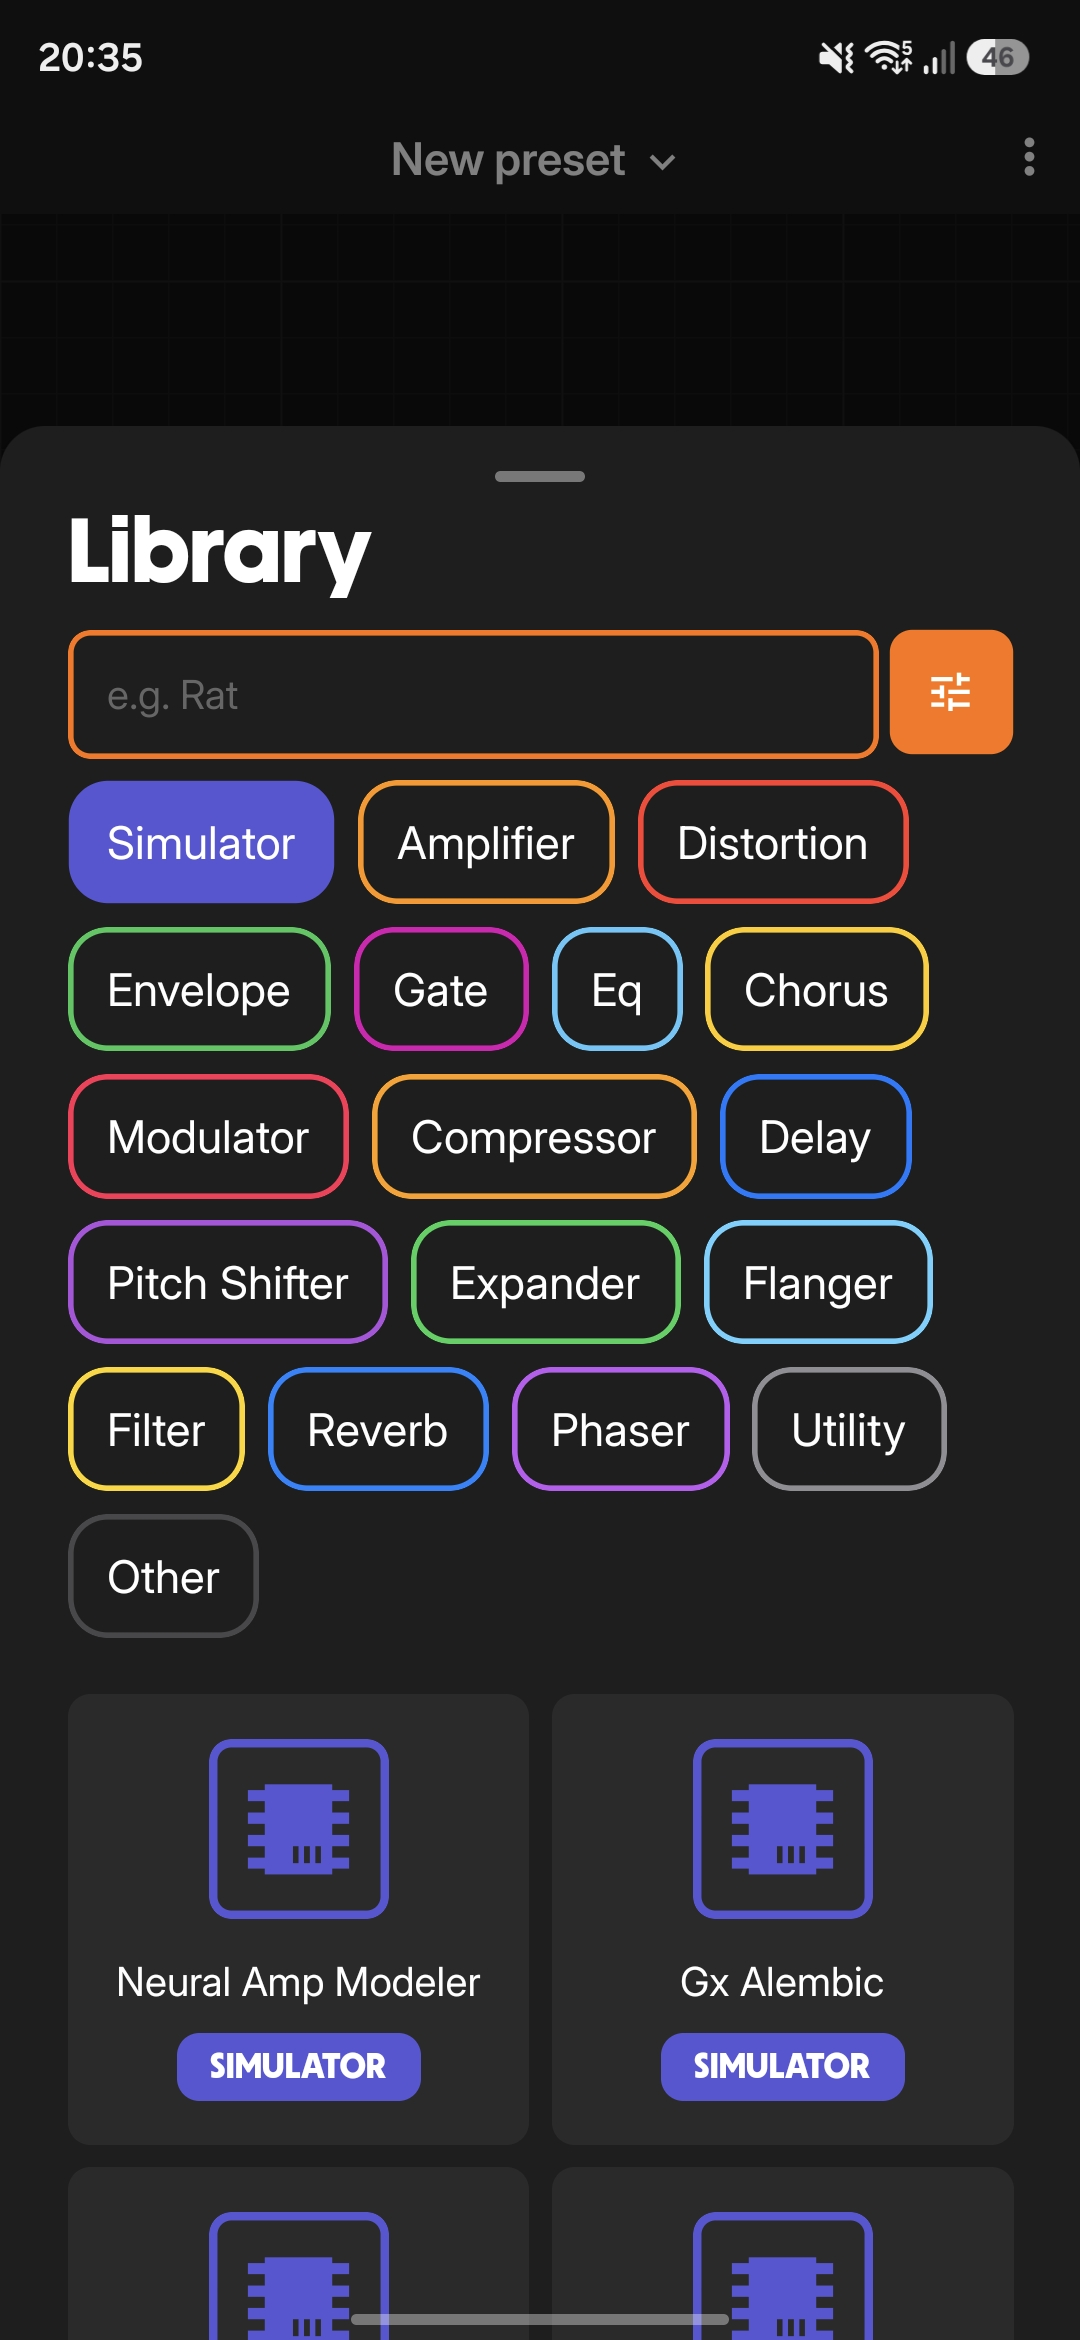
\includegraphics[width=\textwidth]{Screenshot_20260727_203505_Guitarian.jpg}
    \caption{Widok dolnego panelu z biblioteką dostępnych
    efektów[źródło własne]}
    \label{fig:plugins_library_sheet}
  \end{minipage}
\end{figure}

W celu dodania efektu do łańcucha efektów, należy skorzystać z
przycisku akcji umiejscowionego w prawym dolnym rogu ekranu.
Interakcja z nim powoduje płynne wysunięcie się dolnego panelu (ang.
  \textit{bottom sheet}, widocznego na Rysunku
\ref{fig:plugins_library_sheet}), który wyświetla listę wszystkich
dostępnych w systemie wtyczek. Odszukanie pożądanego efektu może
zostać zrealizowane na kilka sposobów: poprzez ręczne przewijanie
biblioteki, wykorzystanie wbudowanej wyszukiwarki tekstowej lub
zastosowanie filtrów kategorii. Te ostatnie pozwalają na
natychmiastowe zawężenie prezentowanej listy wyłącznie do modułów
należących do zaznaczonych grup (np. przestery, efekty modulacyjne).
Zlecenie załadowania wybranej wtyczki do silnika audio odbywa się w
sposób intuicyjny - poprzez pojedyncze dotknięcie (ang. \textit{tap})
odpowiadającego jej kafelka.

Po pomyślnym załadowaniu wtyczek i zamknięciu dolnego panelu, oczom
użytkownika prezentuje się wizualizacja aktualnego łańcucha efektów.
Przykładowa trasa sygnału została zaprezentowana na Rysunku
\ref{fig:main_screen}

\begin{figure}[H]
  \centering
  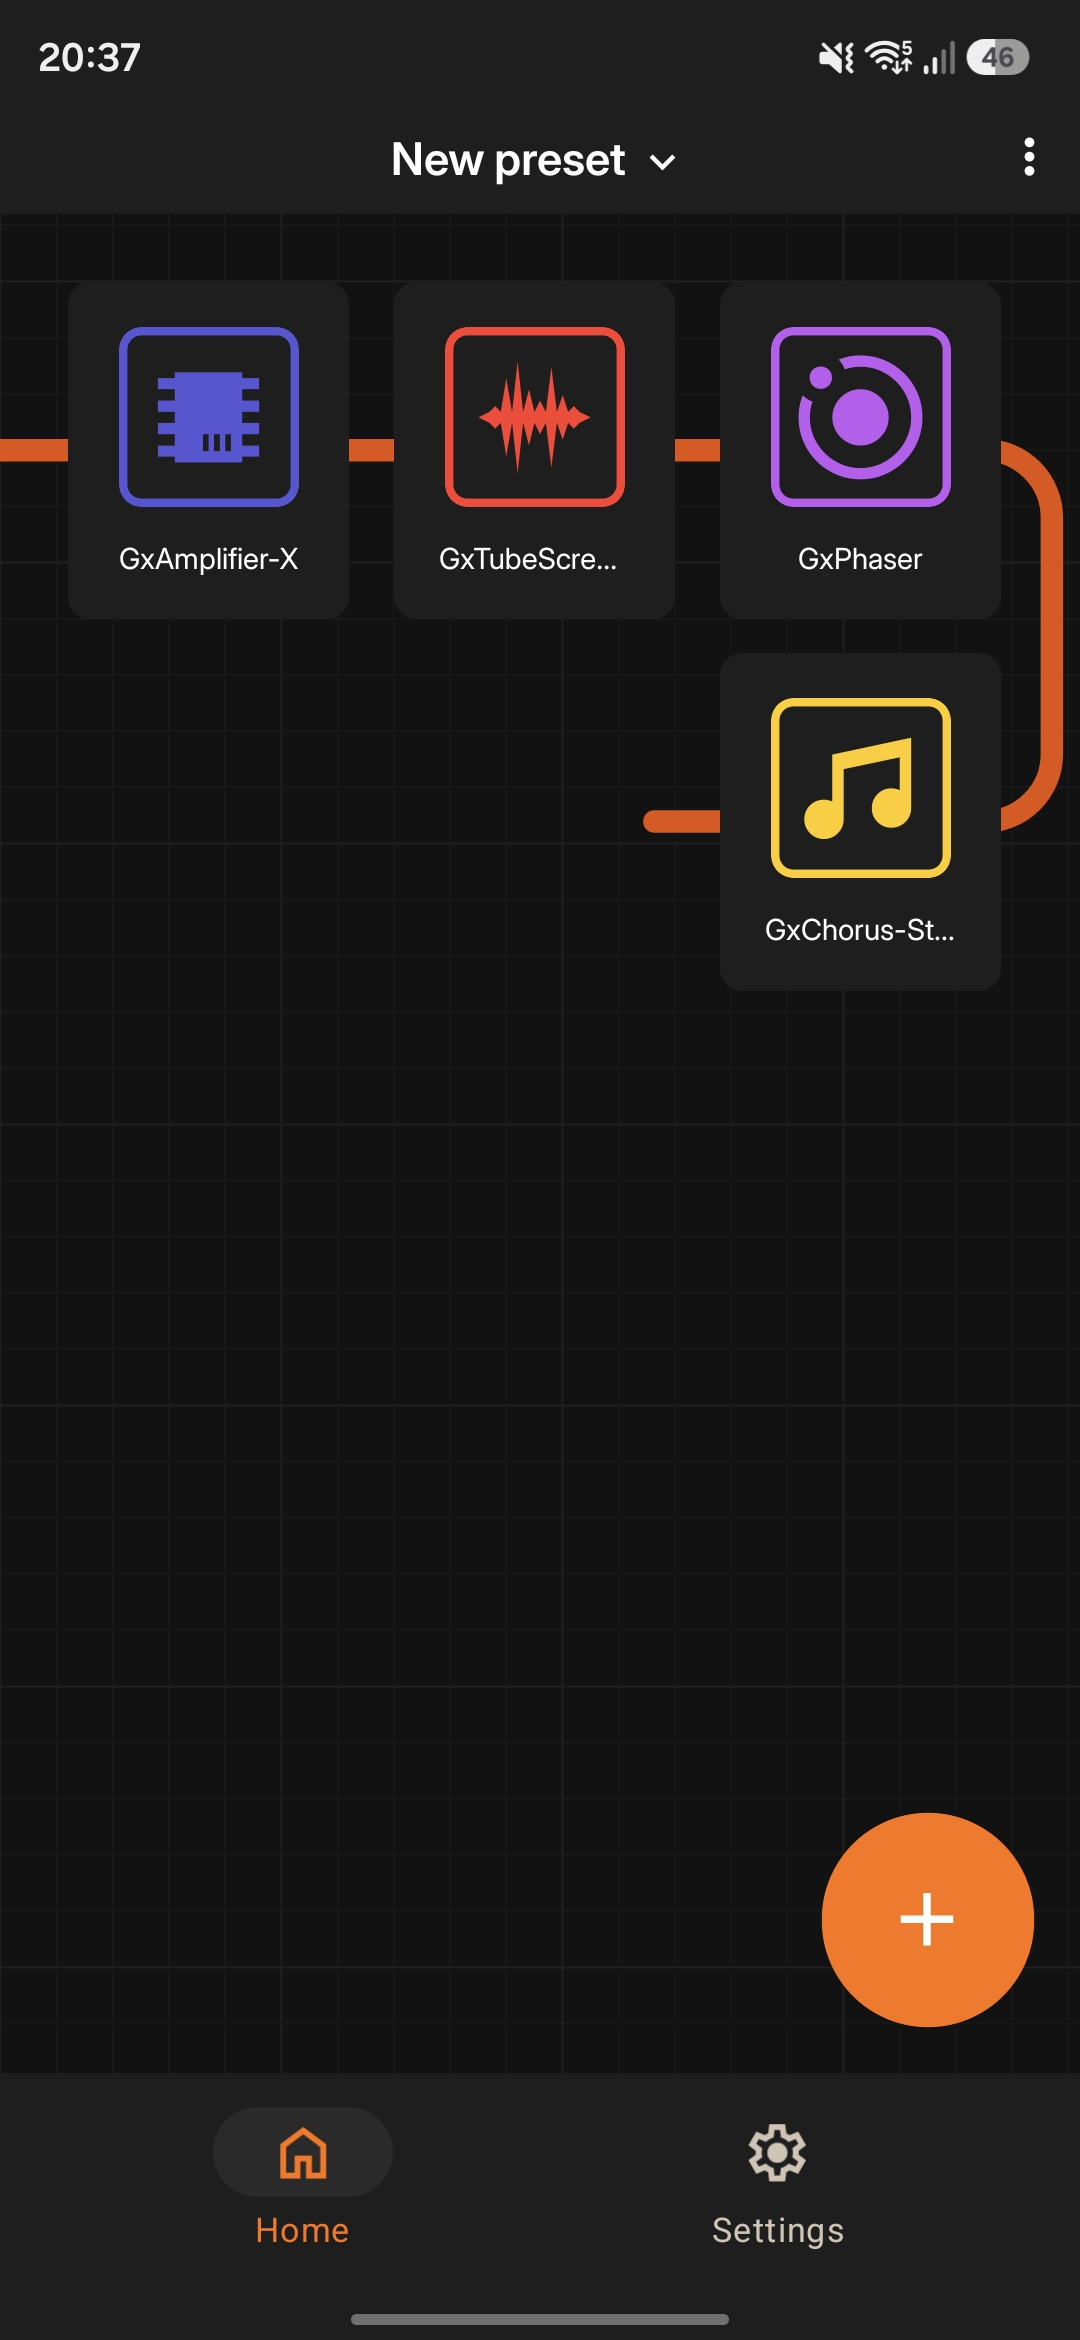
\includegraphics[width=0.5\textwidth]{Screenshot_20260727_203731_Guitarian.jpg}
  \caption{Główny ekran z wizualną reprezentacją obecnego łańcucha
  efektów[źródło własne]}
  \label{fig:main_screen}
\end{figure}

\subsection{Dostosowywanie parametrów wtyczek}
Po pomyślnym dodaniu wtyczki do łańcucha efektów, użytkownik może
kontrolować jej parametry przetwarzania sygnału. Pojedyncze
dotknięcie kafelka reprezentującego aktywną wtyczkę powoduje
wysunięcie dedykowanego panelu konfiguracyjnego, który został
zaprezentowany na Rysunku \ref{fig:params_sheet}.

\begin{figure}[H]
  \centering
  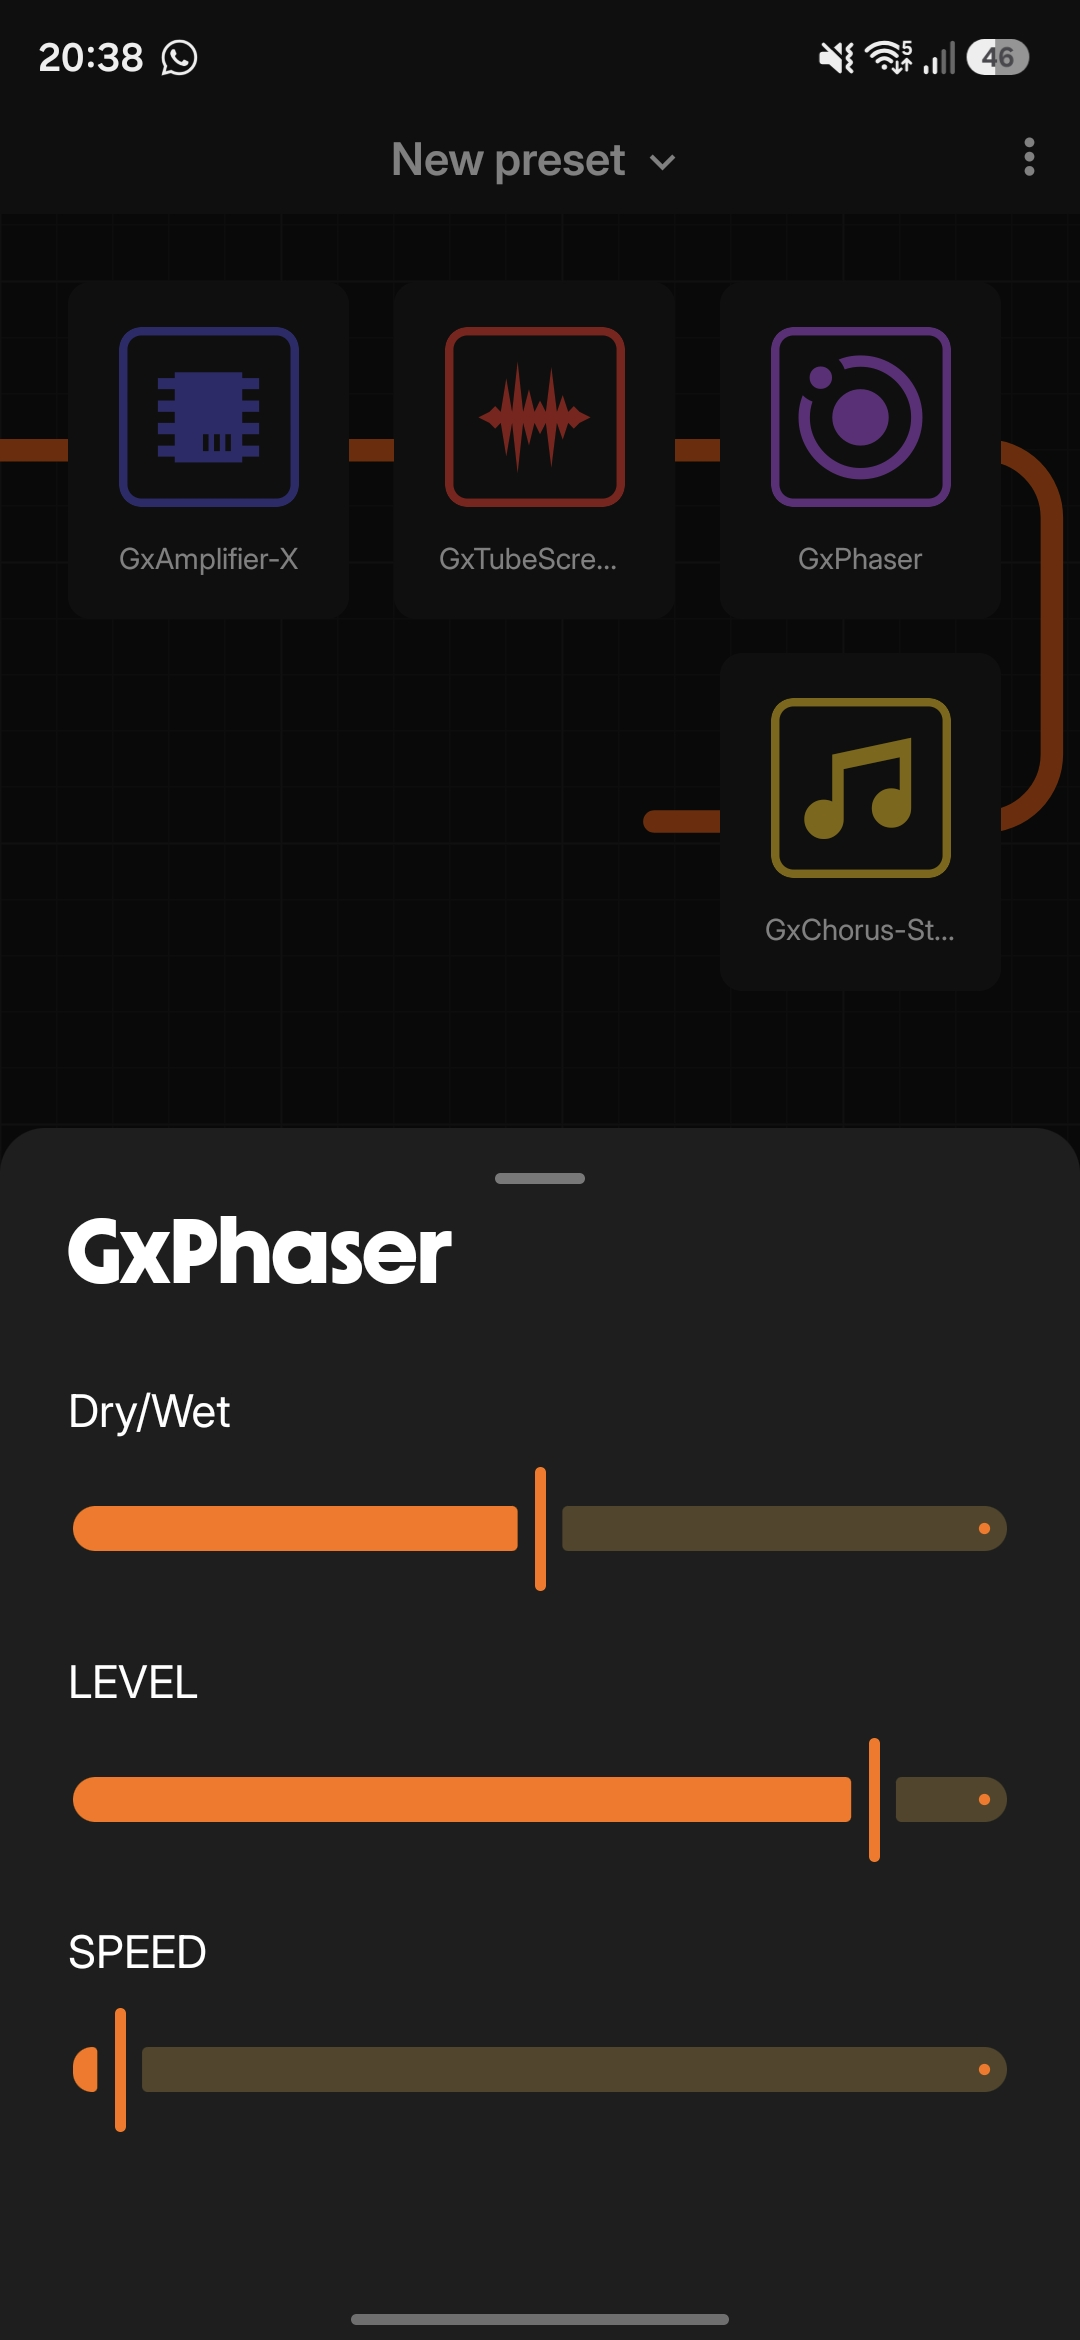
\includegraphics[width=0.5\textwidth]{Screenshot_20260727_203842_Guitarian.jpg}
  \caption{Panel konfiguracji parametrów wtyczki[źródło własne]}
  \label{fig:params_sheet}
\end{figure}

Manipulacja udostępnionymi kontrolkami skutkuje natychmiastowym
wysłaniem zaktualizowanych wartości do silnika audio, co pozwala
użytkownikowi na płynne odsłuchiwanie i ewaluację brzmienia w czasie
rzeczywistym. Co istotne, interfejs tego widoku jest generowany w
sposób w pełni dynamiczny, na podstawie metadanych dostarczanych
przez samą wtyczkę. W zależności od zdefiniowanego typu danego
parametru, aplikacja renderuje odpowiednie elementy graficzne:
klasyczne suwaki dla wartości ciągłych zmiennoprzecinkowych lub
dyskretnych, przełączniki dwustanowe dla wartości logicznych, bądź
też rozwijane listy wyboru dla parametrów wyliczeniowych.

\subsection{Zarządzanie kolejnością i usuwanie}
Z poziomu głównego obszaru roboczego użytkownik dysponuje
możliwościami modyfikacji kolejności aktywnych wtyczek oraz ich
usuwania z trasy sygnału. Konfiguracja pozycji w łańcuchu opiera się
na powszechnie stosowanym, intuicyjnym wzorcu interakcji przeciągnij
i upuść (ang. \textit{drag and drop}). Wykonanie gestu dłuższego
przytrzymania (ang. \textit{long press}) na wybranym kafelku włącza
tryb swobodnego przenoszenia, pozwalając na przemieszczenie elementu
w docelowe miejsce łańcucha. Po zwolnieniu kafelka, zaktualizowana
struktura jest natychmiastowo przesyłana do silnika audio w celu
zaaplikowania zmian. Działanie tego mechanizmu zilustrowano na
rysunku \ref{fig:card_drag}.

\begin{figure}[H]
  \centering
  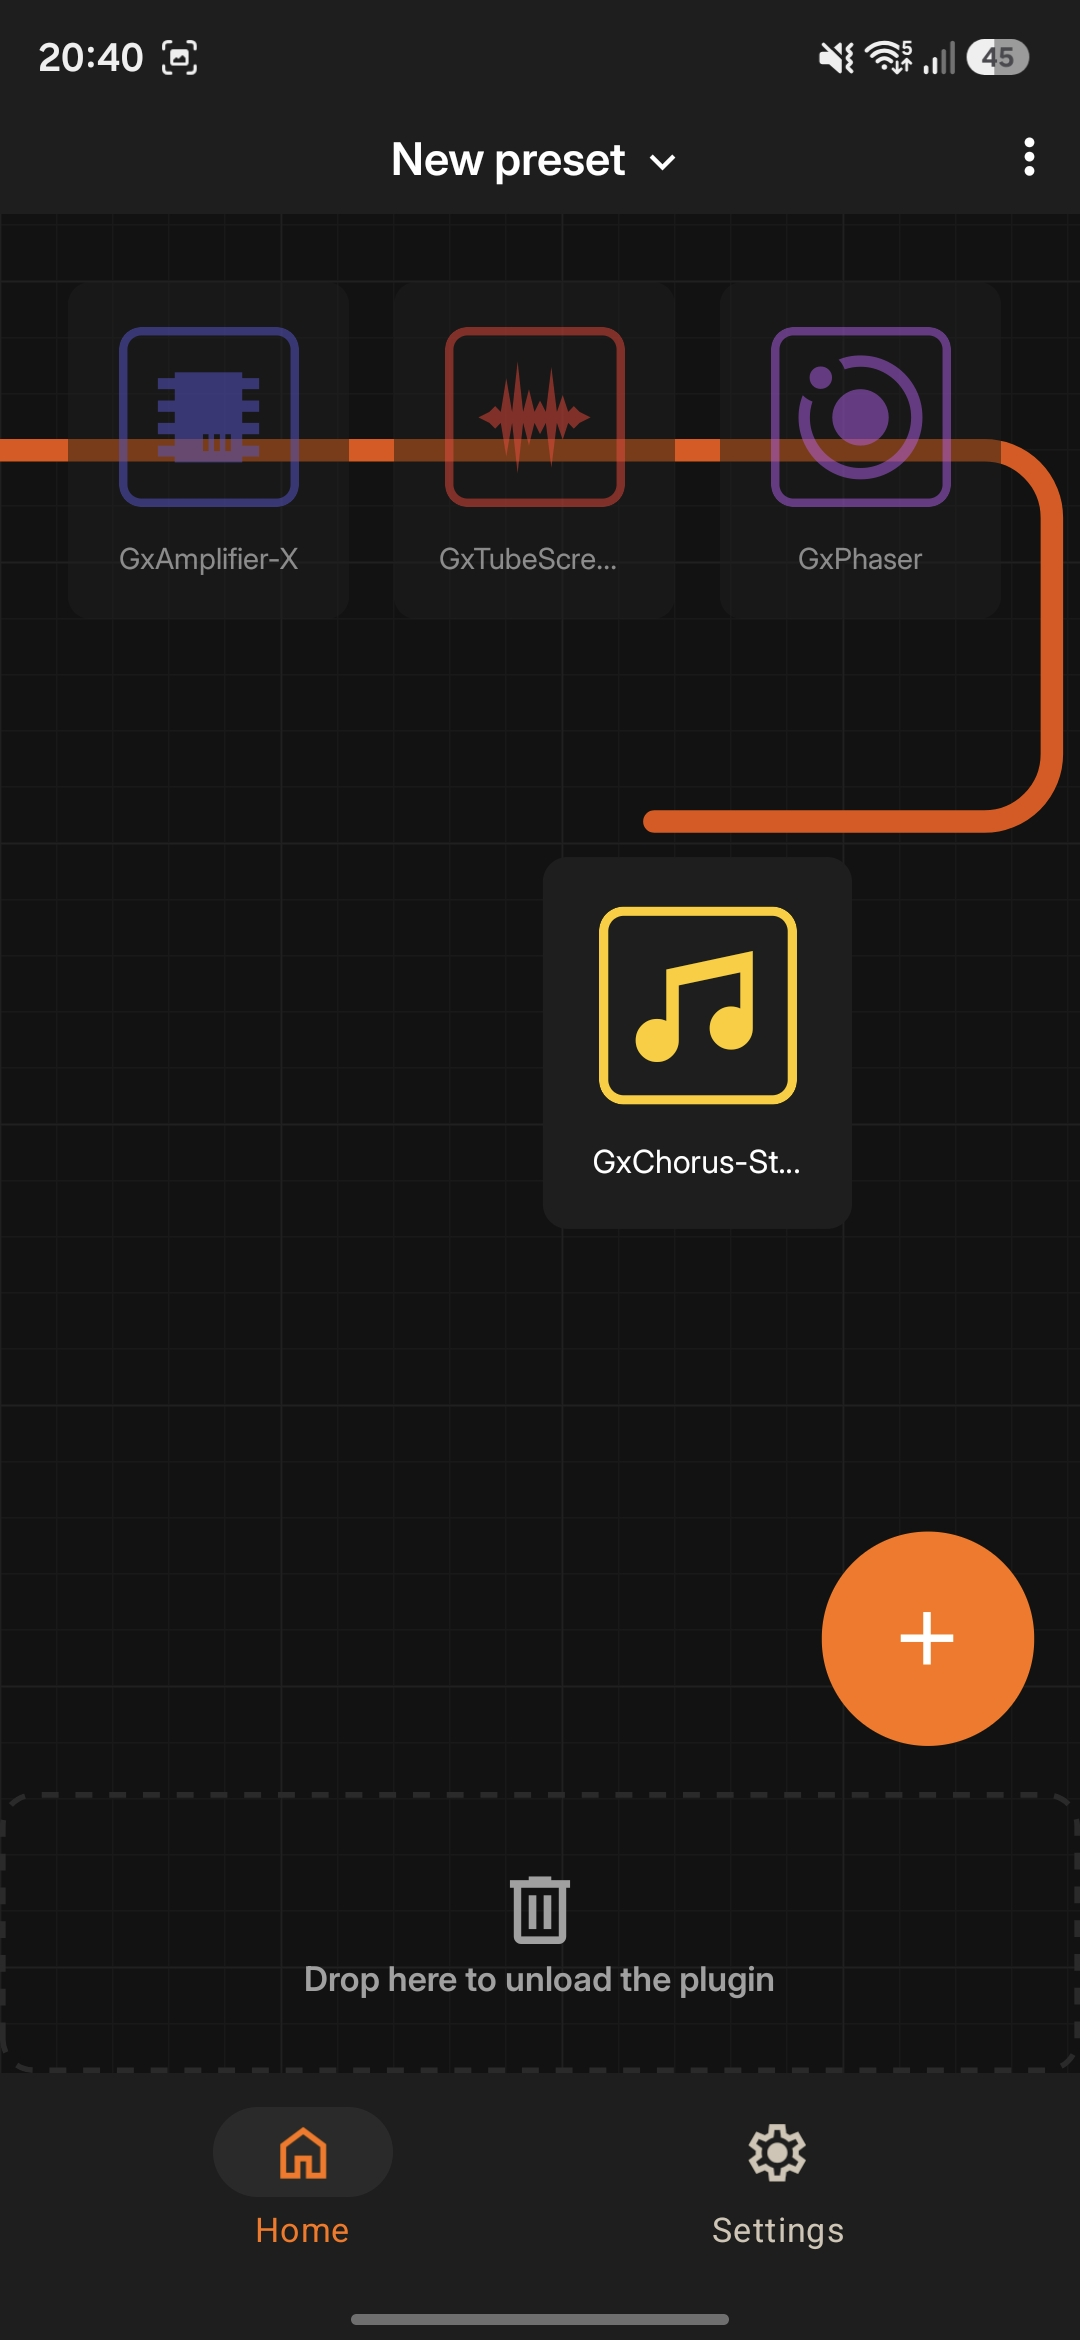
\includegraphics[width=0.5\textwidth]{Screenshot_20260727_204053_Guitarian.jpg}
  \caption{Zarządzanie położeniem wtyczki w łańcuchu efektów[źródło własne]}
  \label{fig:card_drag}
\end{figure}

Alternatywnie, podczas wykonywania gestu przenoszenia, użytkownik ma
możliwość całkowitego usunięcia wtyczki z łańcucha. Operację tę
realizuje się poprzez przeciągnięcie kafelka i upuszczenie go w
dedykowanej strefie usuwania, która dynamicznie pojawia się w dolnej
części ekranu.

Użytkownik ma również możliwość szybkiego usunięcia wszystkich
wtyczek z trasy sygnału przez dotknięcie odpowiedniej opcji w
otwieranym przyciskiem trzech kropek menu widocznym na Rysunku
\ref{fig:remove_all}, a następnie potwierdzeniu tej akcji.

\begin{figure}[H]
  \centering
  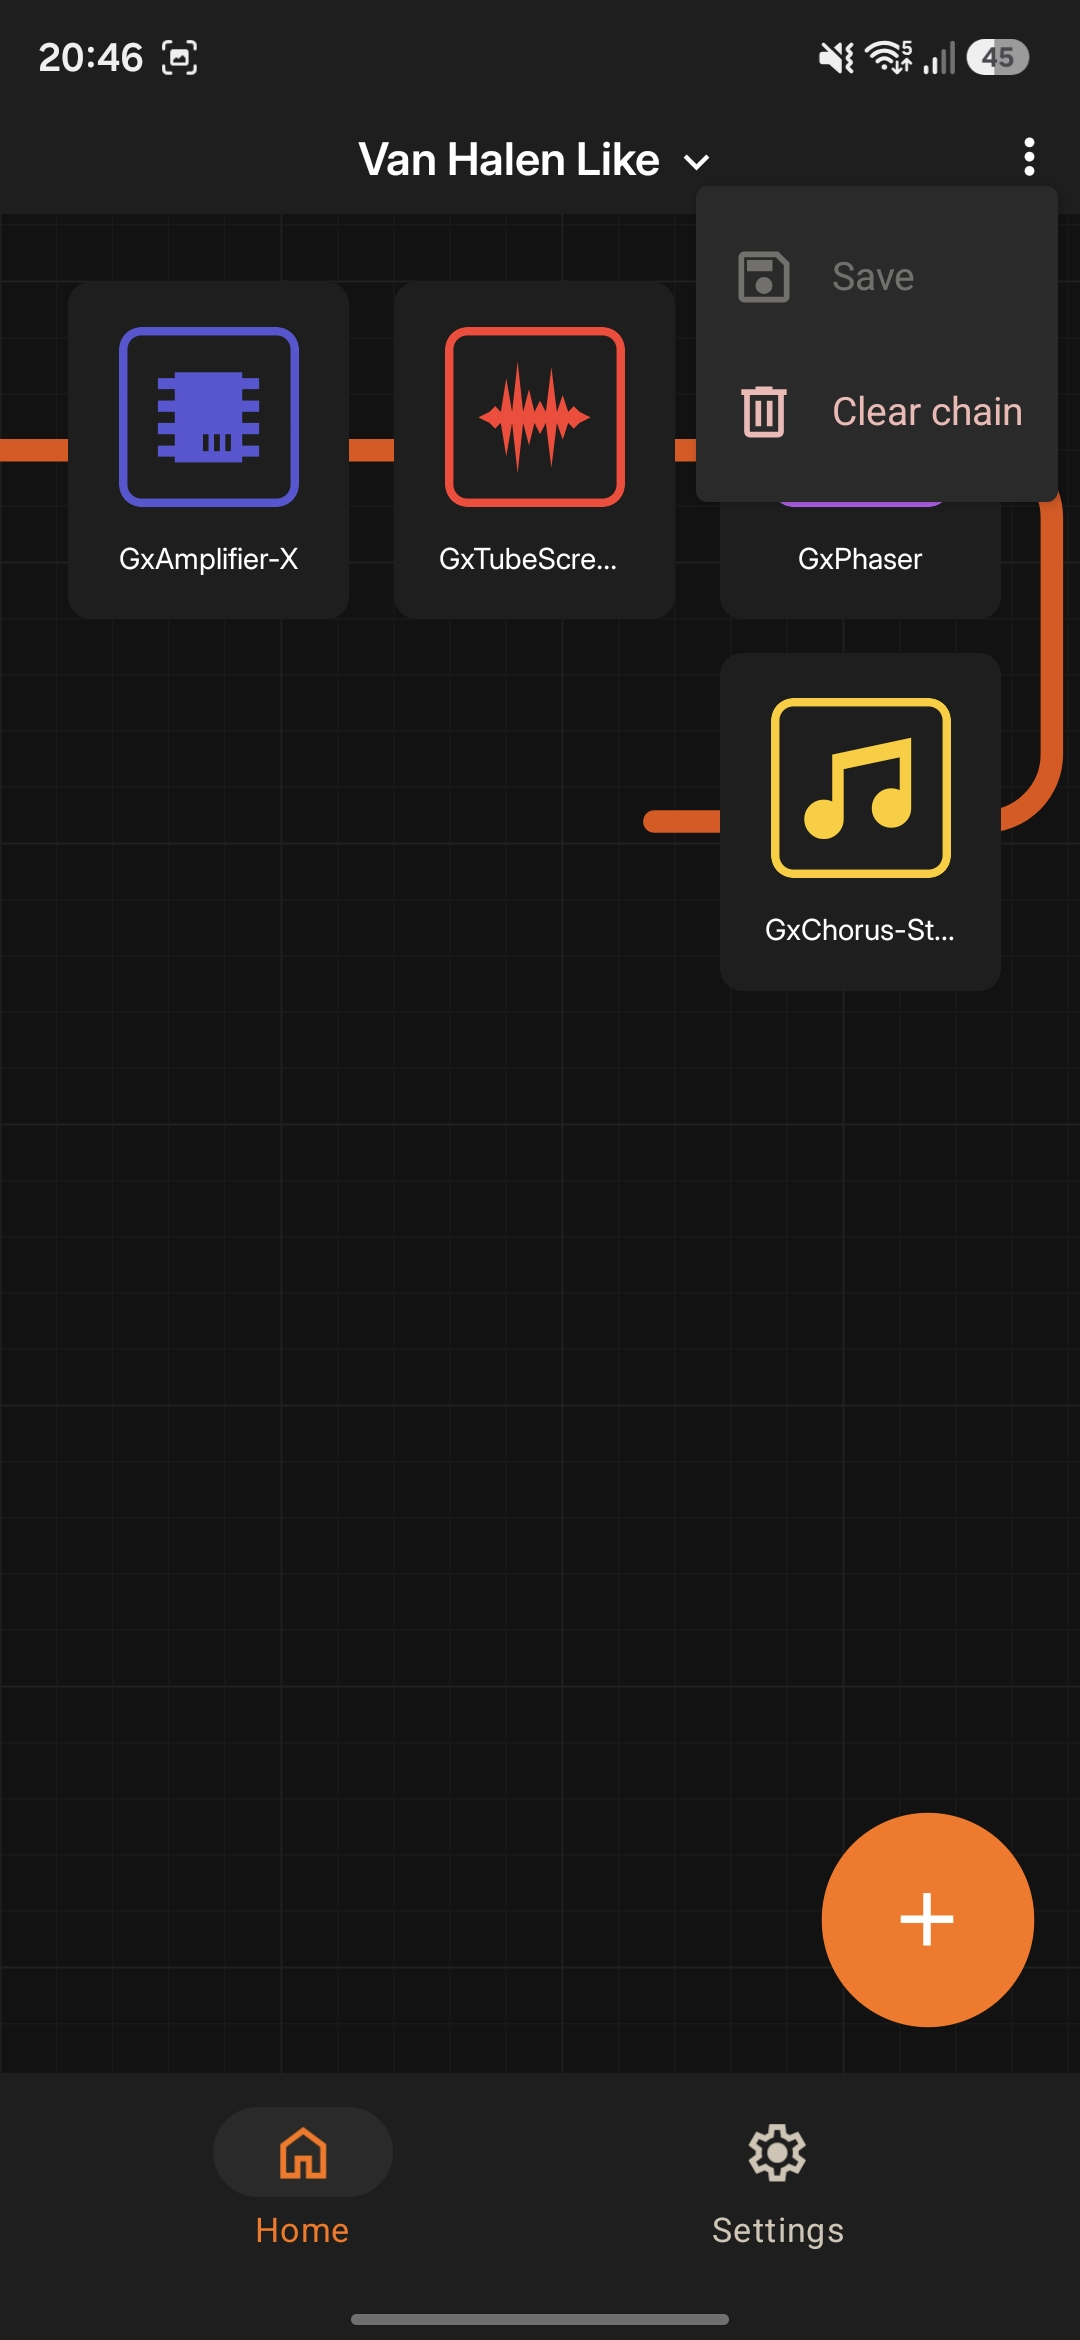
\includegraphics[width=0.5\textwidth]{Screenshot_20260727_204651_Guitarian.jpg}
  \caption{Usuwanie wszystkich aktywnych wtyczek z łańcucha
  efektów[źródło własne]}
  \label{fig:remove_all}
\end{figure}

\subsection{Zapisywanie ulubionego brzmienia}
Po precyzyjnym skonfigurowaniu łańcucha przetwarzania sygnału,
użytkownik ma możliwość trwałego zapisania jego kompletnego stanu.
Funkcjonalność ta pozwala na późniejsze, natychmiastowe przywrócenie
ulubionego brzmienia, eliminując potrzebę żmudnego, ręcznego
odtwarzania wszystkich ustawień.

W celu utrwalenia aktualnej konfiguracji należy wybrać opcję
\textit{Save} z menu kontekstowego. Wywołuje to modalne okno
dialogowe (ang. \textit{dialog box}), w którym użytkownik może
wprowadzić unikalną nazwę dla tworzonego zestawu ustawień (ang.
\textit{preset}). Etap ten został przedstawiony na rysunku
\ref{fig:create_preset}.

\begin{figure}[H]
  \centering
  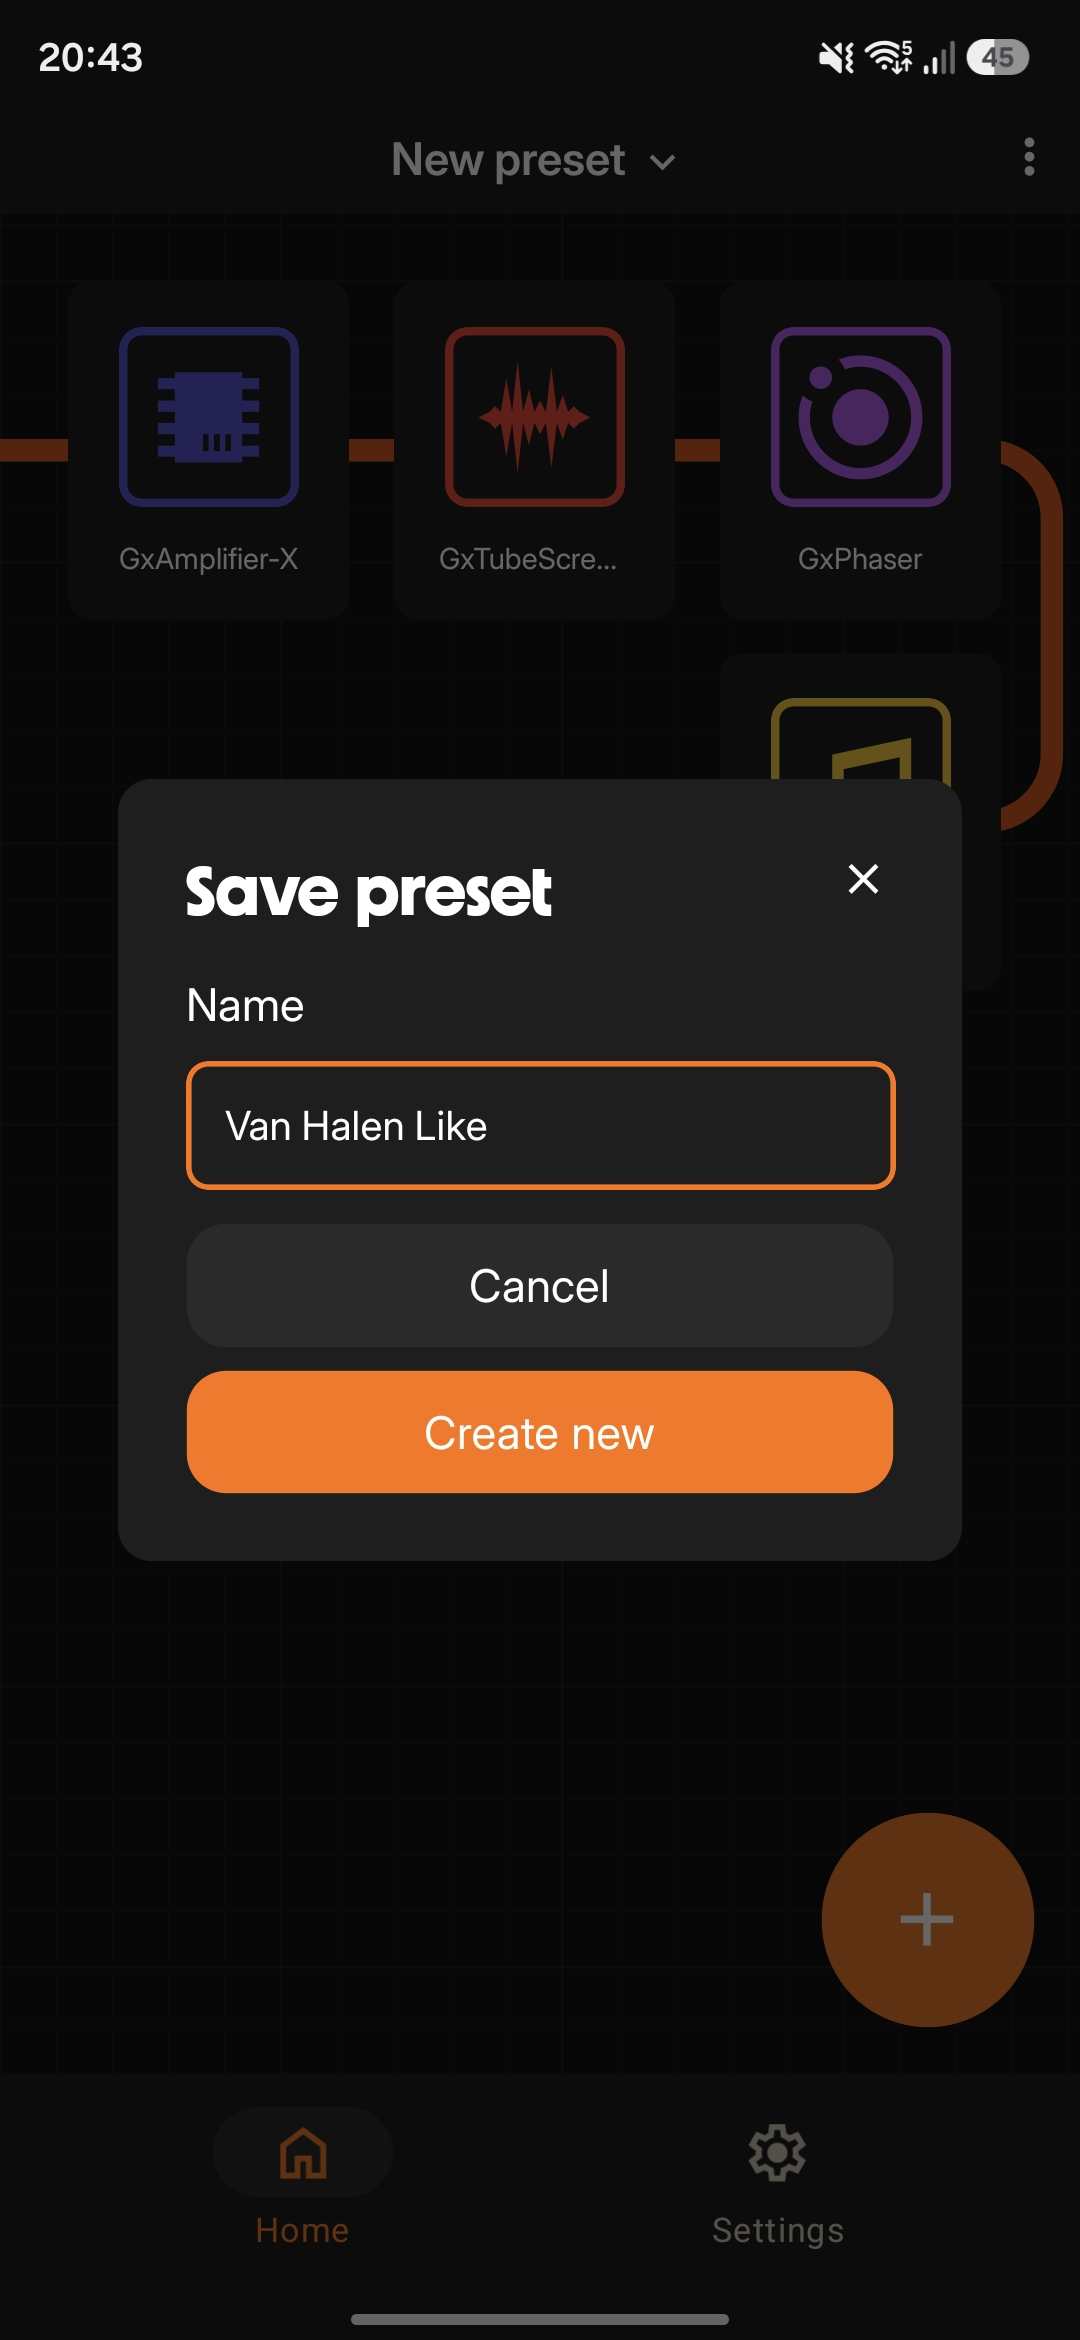
\includegraphics[width=0.5\textwidth]{Screenshot_20260727_204349_Guitarian.jpg}
  \caption{Okno dialogowe tworzenia nowego zestawu ustawień
  (presetu)[źródło własne]}
  \label{fig:create_preset}
\end{figure}

Po pomyślnym zatwierdzeniu zapisu, nagłówek głównego ekranu aplikacji
zostaje zaktualizowany, informując o nazwie obecnie aktywnego
profilu. Bezpośrednia interakcja z tym nagłówkiem (pojedyncze
dotknięcie) skutkuje wysunięciem dolnego panelu (widocznego na
rysunku \ref{fig:presets_sheet}), prezentującego zbiór wszystkich
wcześniej zapisanych konfiguracji.

\begin{figure}[H]
  \centering
  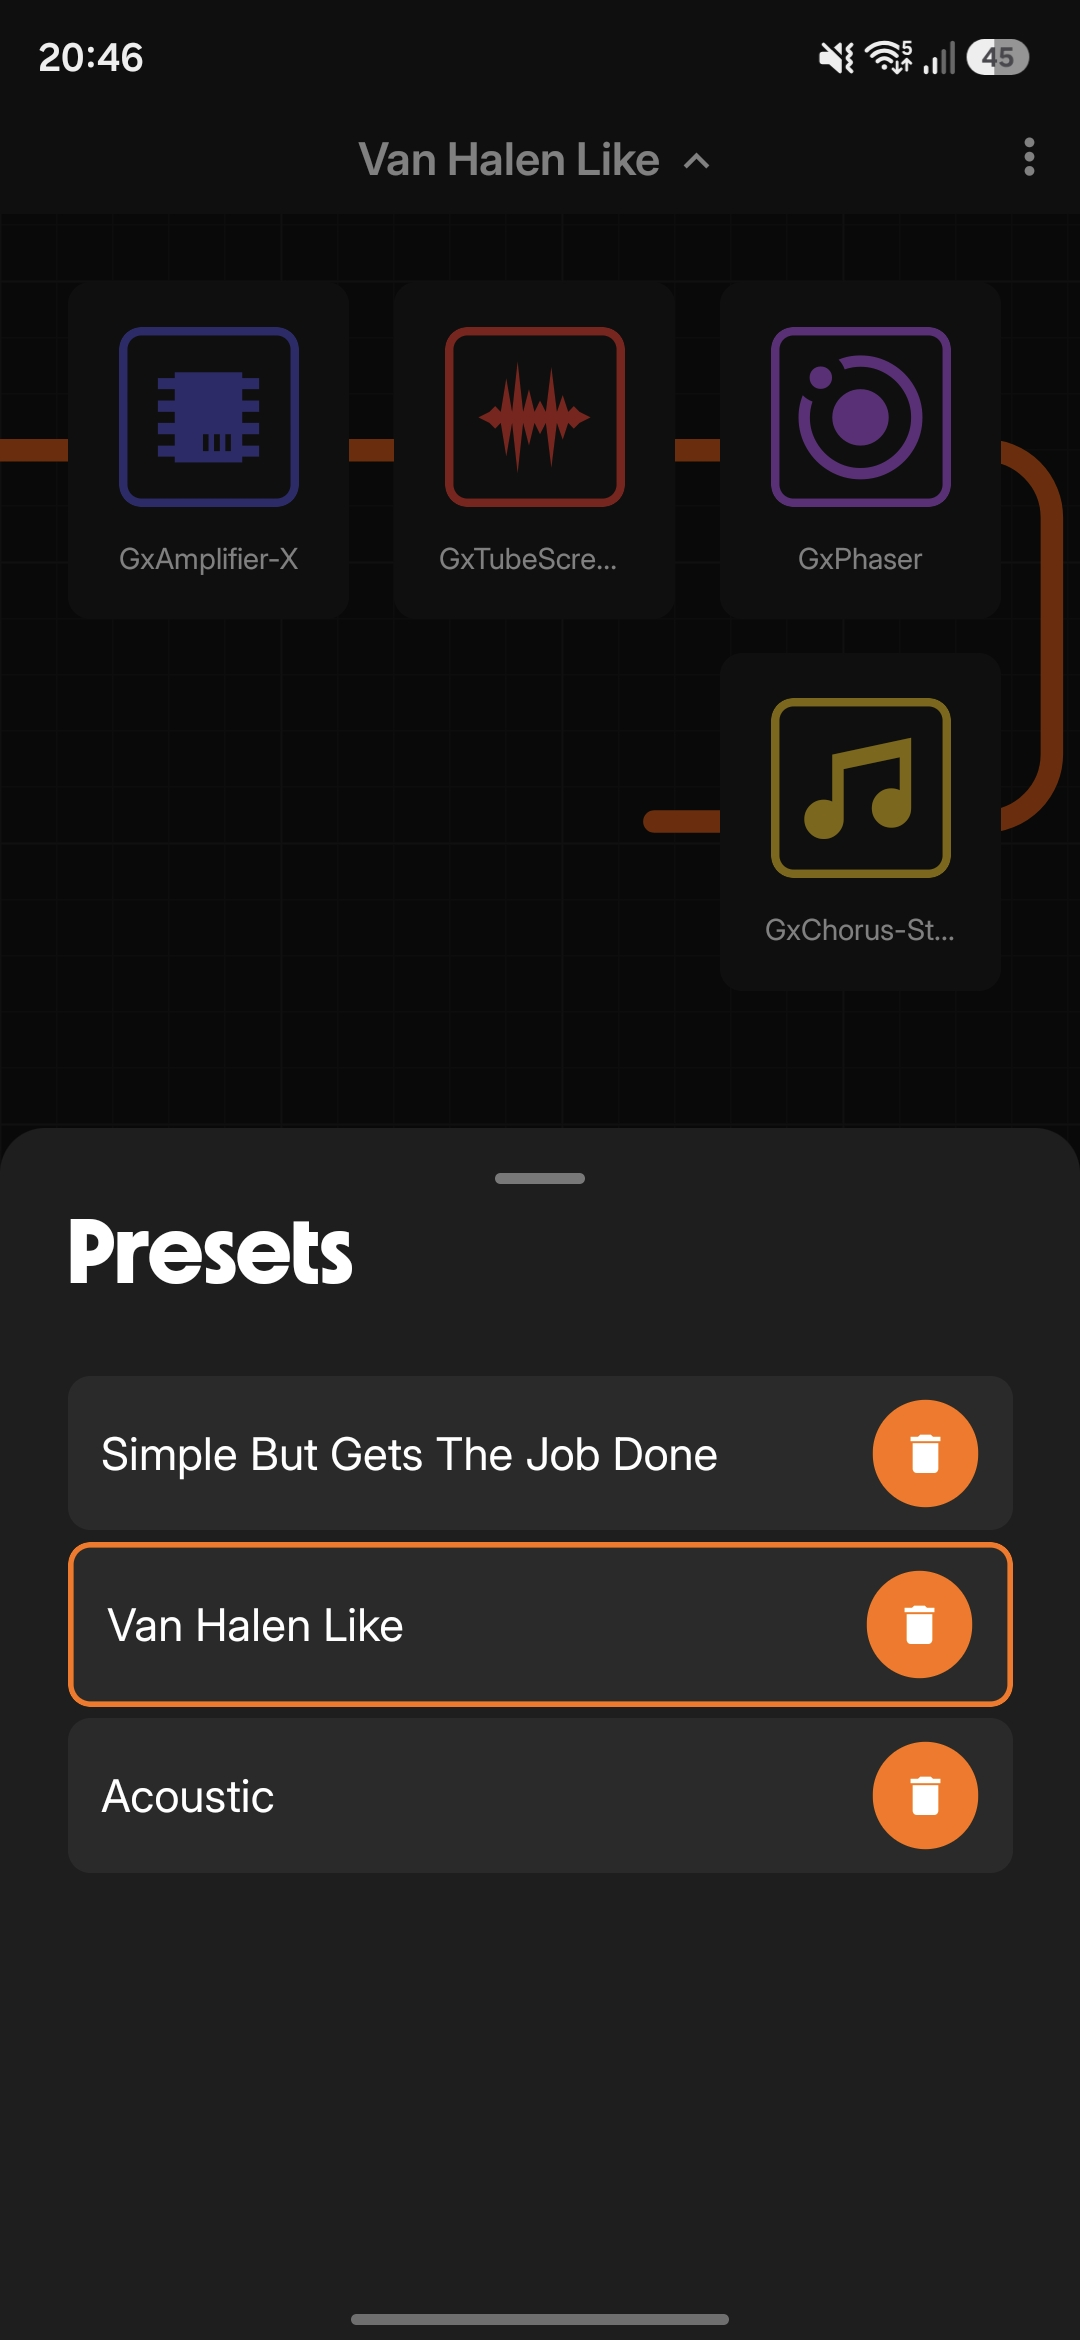
\includegraphics[width=0.5\textwidth]{Screenshot_20260727_204628_Guitarian.jpg}
  \caption{Widok panelu z listą dostępnych zestawów ustawień[źródło własne]}
  \label{fig:presets_sheet}
\end{figure}

Z poziomu omawianego panelu użytkownik może zainicjować proces
ładowania wybranego presetu lub dokonać jego trwałego usunięcia.
Mechanizm aktualizacji już istniejącego zestawu jest bardzo prosty i
sprowadza się do naniesienia pożądanych zmian w łańcuchu efektów, a
następnie ponownego wywołania procedury zapisu. W oknie dialogowym
nazwa aktywnego ustawienia jest uzupełniana automatycznie, co po
zatwierdzeniu skutkuje nadpisaniem starych wartości. Wprowadzenie w
tym miejscu innej nazwy zainicjuje z kolei utworzenie zupełnie nowego
ustawienia.

\section{Zarządzanie ustawieniami silnika audio}
Z perspektywy użyteczności oraz wygody obsługi, kluczowym wymaganiem
jest zapewnienie użytkownikowi możliwości konfiguracji
najważniejszych parametrów systemu bez konieczności bezpośredniej
ingerencji w środowisko uruchomieniowe silnika audio (np. za
pośrednictwem SSH). Z tego też powodu, w aplikacji klienckiej
zaimplementowano ekran ustawień, który oddaje kontrolę nad kluczowymi
parametrami z poziomu aplikacji mobilnej. Ekran ten został
zaprezentowany na rysunku \ref{fig:settings_screen}.

\begin{figure}[H]
  \centering
  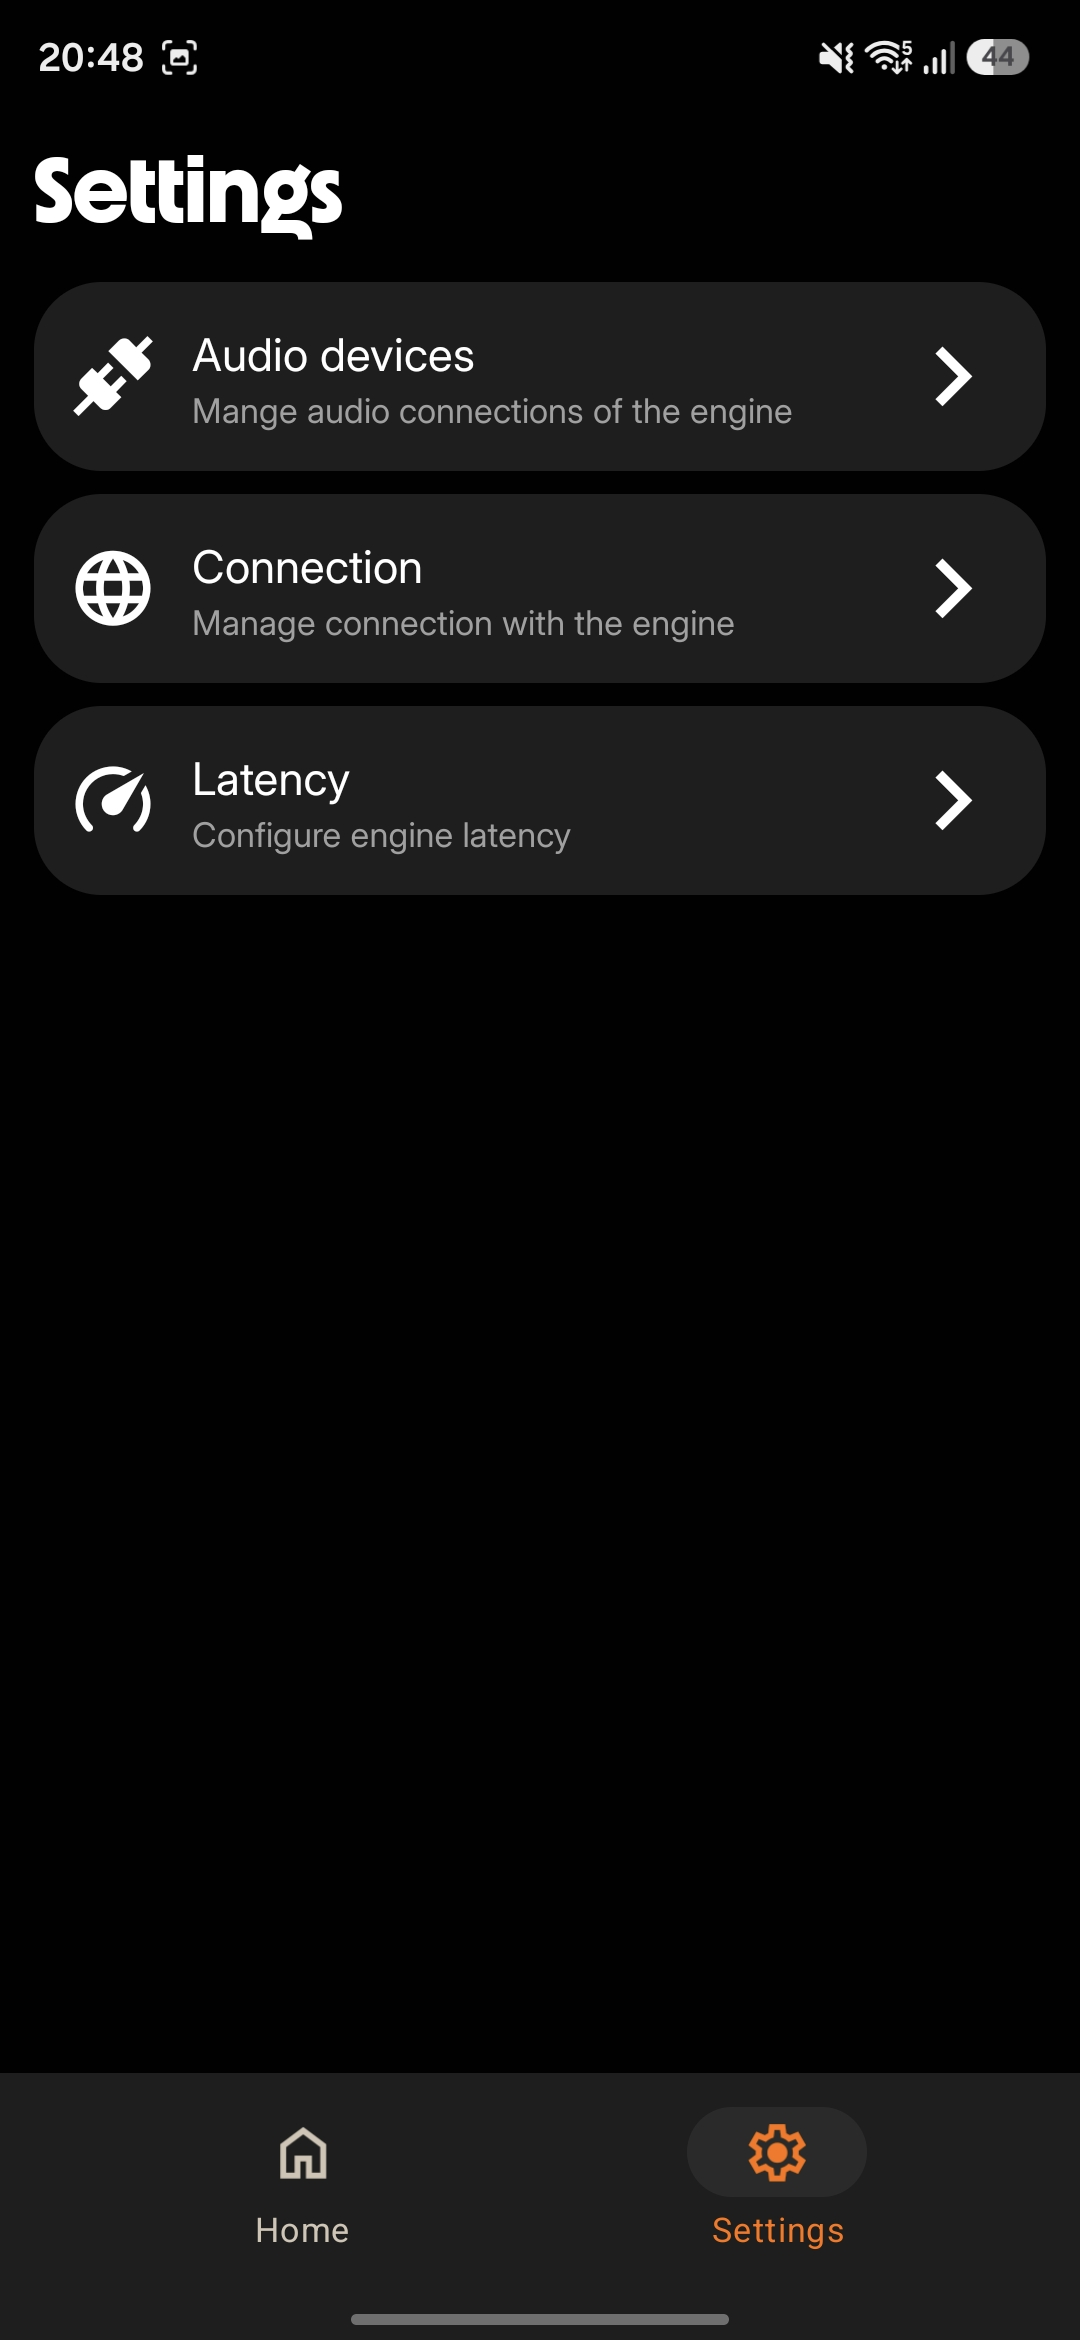
\includegraphics[width=0.5\textwidth]{Screenshot_20260727_204839_Guitarian.jpg}
  \caption{Ekran ustawień[źródło własne]}
  \label{fig:settings_screen}
\end{figure}

\subsection{Konfiguracja aktywnych urządzeń wejścia i wyjścia}
Współczesne zewnętrzne interfejsy audio rzadko ograniczają się do
jednego, konkretnego toru sygnału. Większość z nich dysponuje wieloma
wejściami (np. wejściem mikrofonowym i instrumentalnym) oraz wieloma
wyjściami (pozwalającymi na niezależne podłączenie monitorów
odsłuchowych i słuchawek). Z punktu widzenia prostoty użytkowania
systemu, absolutnie kluczowe było zaimplementowanie mechanizmu
swobodnego zarządzania trasą sygnału. Zaprezentowany na rysunku
\ref{fig:settings_screen-in_out}, ekran pozwala zdecydować, które ze
sprzętowych portów wejściowych ma stanowić źródło sygnału dla
wirtualnego łańcucha efektów, a także na które wyjścia zostanie
skierowany finalny, przetworzony dźwięk. Użytkownik może pokierować
dźwięk jednocześnie na kilka różnych portów wyjściowych.

\begin{figure}[H]
  \centering
  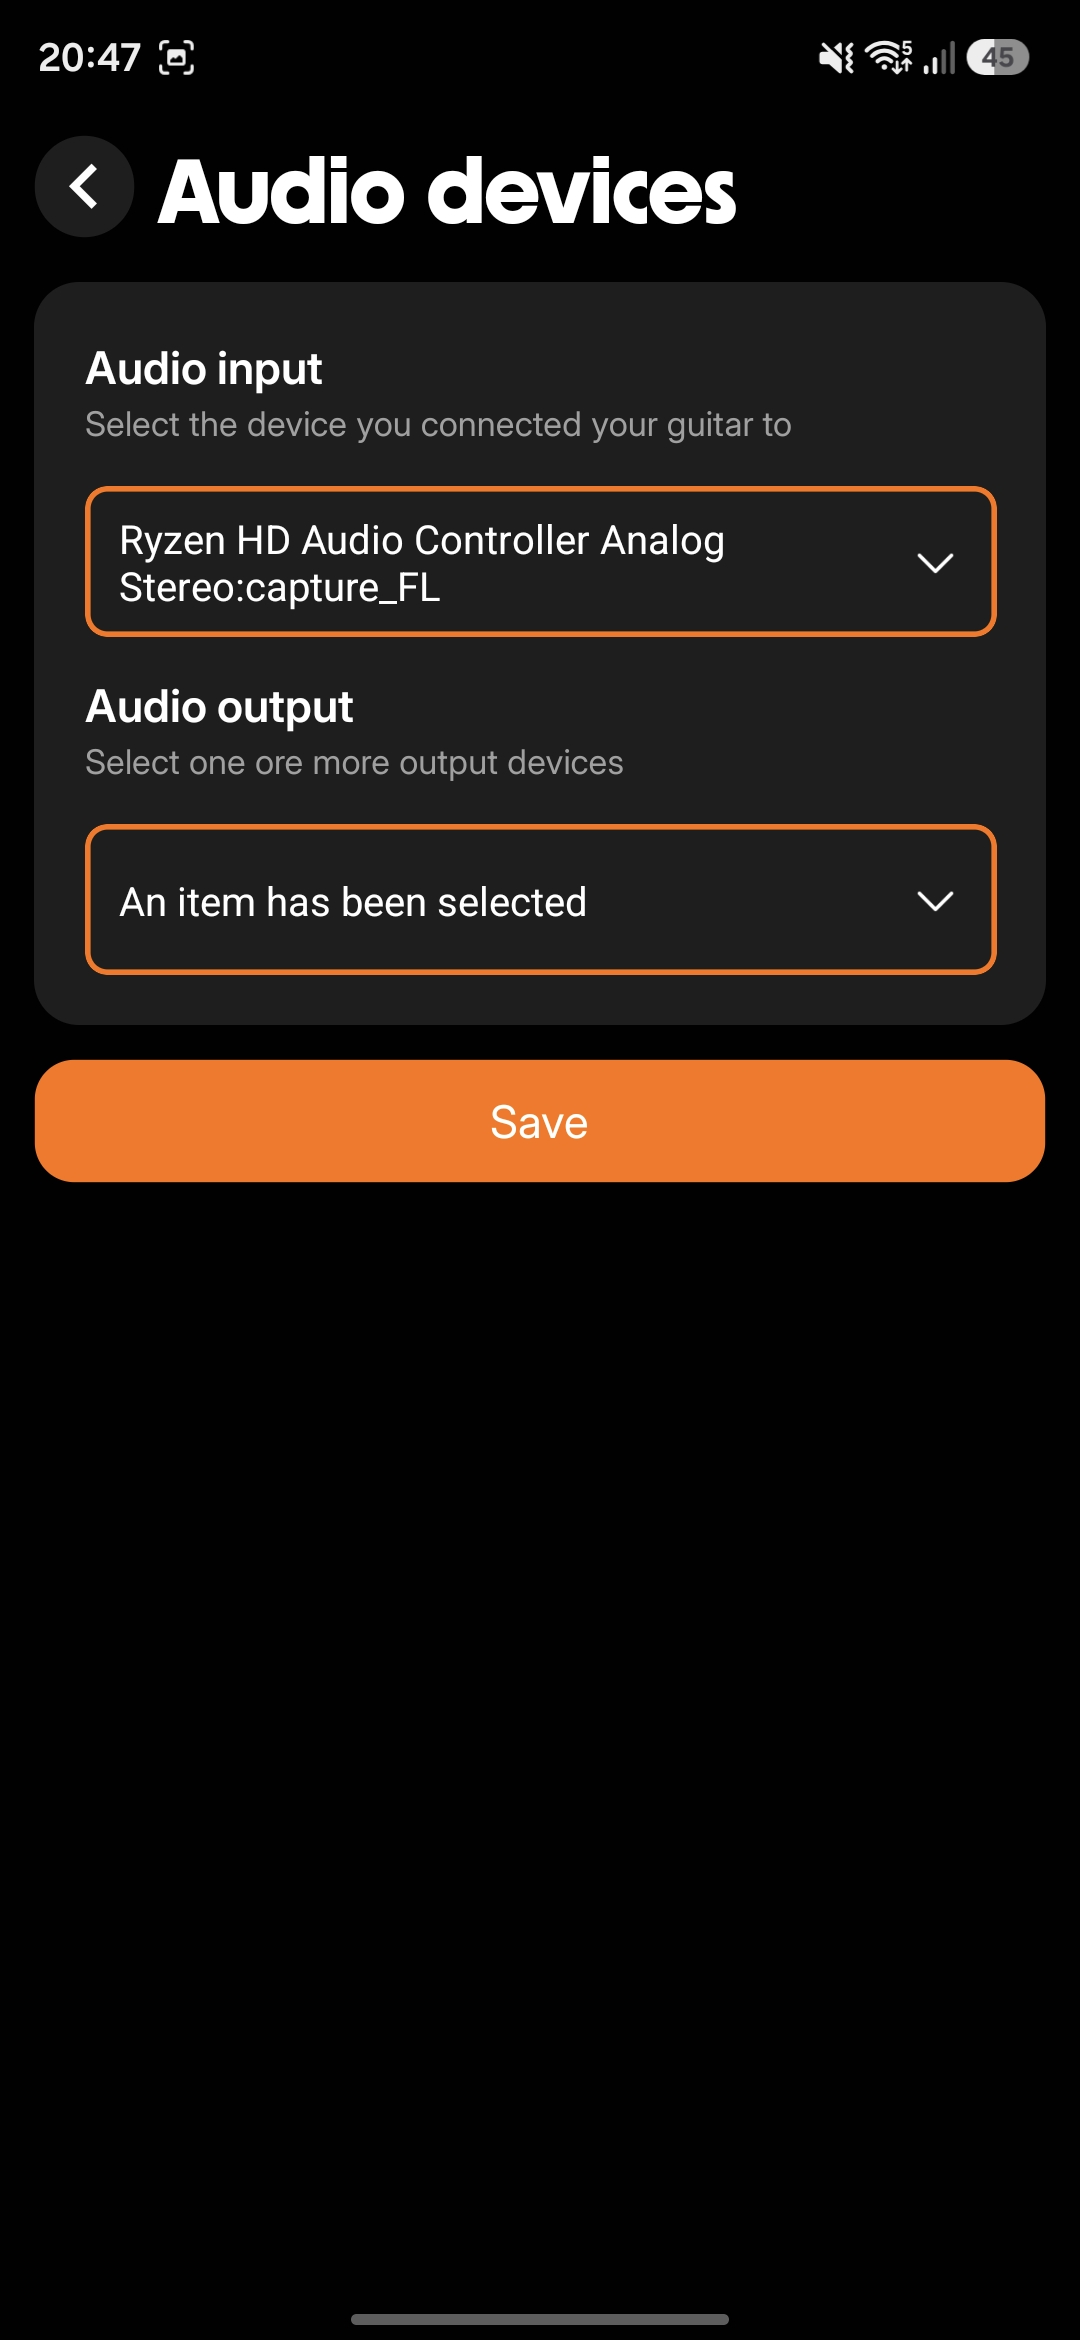
\includegraphics[width=0.5\textwidth]{Screenshot_20260727_204738_Guitarian.jpg}
  \caption{Ekran ustawień - konfiguracja wejść i wyjść[źródło własne]}
  \label{fig:settings_screen-in_out}
\end{figure}

Wybrane przez użytkownika opcje zostaną automatycznie przywołane po
ponownym uruchomieniu silnika audio (pod warunkiem, że skonfigurowane
porty wciąż będą dostępne z perspektywy środowiska uruchomieniowego).

\subsection{Manualna konfiguracja połączenia z serwerem kontrolnym}
W przypadku, gdy proces automatycznej konfiguracji się nie powiedzie
lub użytkownik będzie chciał manualnie zmienić adres serwera
kontrolnego, będzie mógł to osiągnąć z poziomu aplikacji. Na
widocznym na Rysunku \ref{fig:settings_screen-connection_status}
ekranie, użytkownik może zapoznać się z aktualnym statusem
połączenia, a także IP serwera kontrolnego. Po kliknięciu opcji
\textit{Edit}, użytkownikowi prezentowany jest widok ukazany na
Rysunku \ref{fig:settings_screen-connection_edit}.

\begin{figure}[H]
  \centering
  \begin{minipage}[t]{0.45\textwidth}
    \centering
    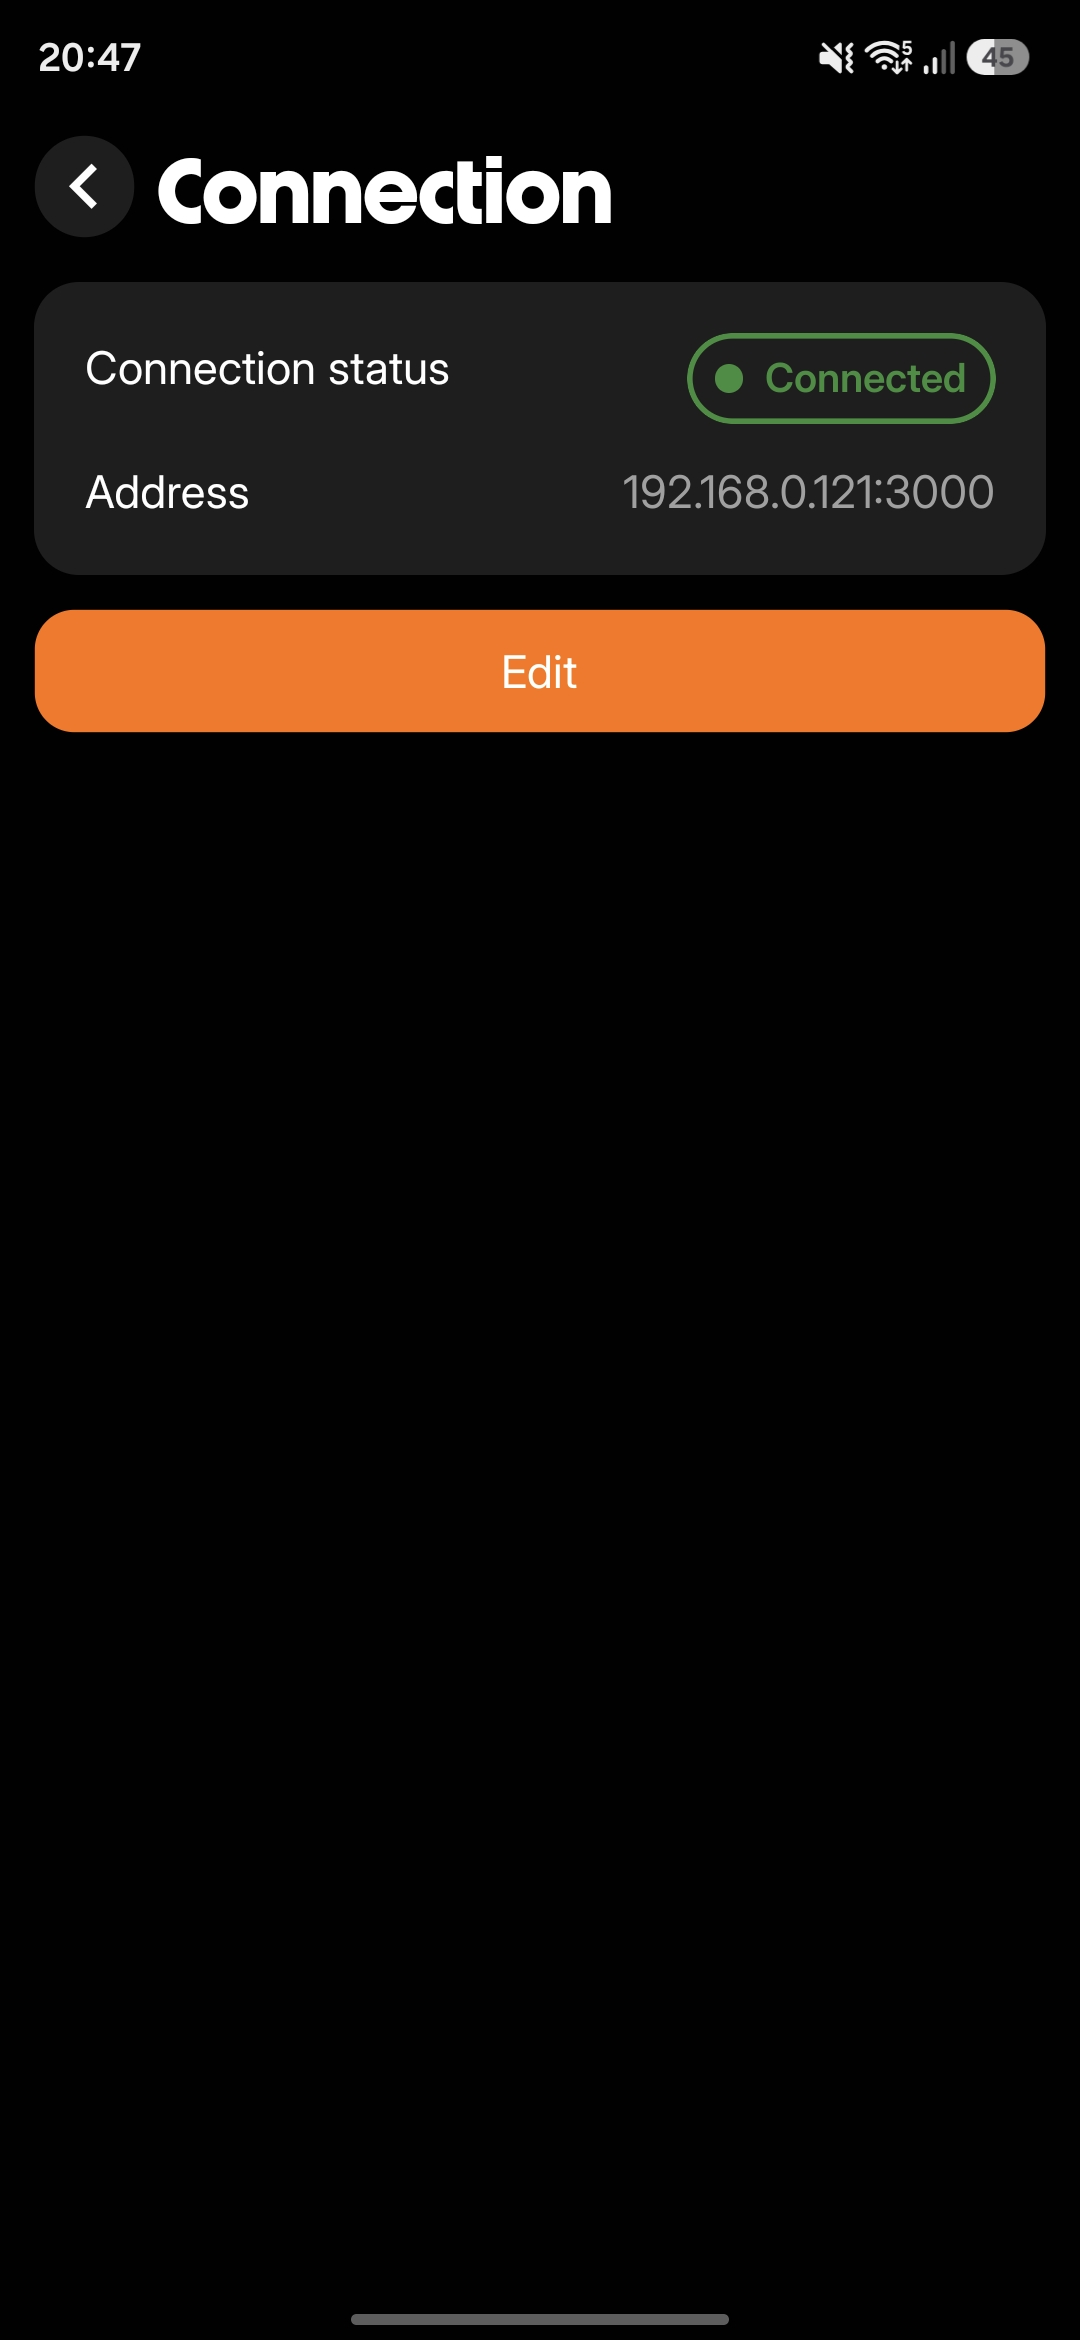
\includegraphics[width=\textwidth]{Screenshot_20260727_204750_Guitarian.jpg}
    \caption{Ekran ustawień - status połączenia[źródło własne]}
    \label{fig:settings_screen-connection_status}
  \end{minipage}
  \hfill
  \begin{minipage}[t]{0.45\textwidth}
    \centering
    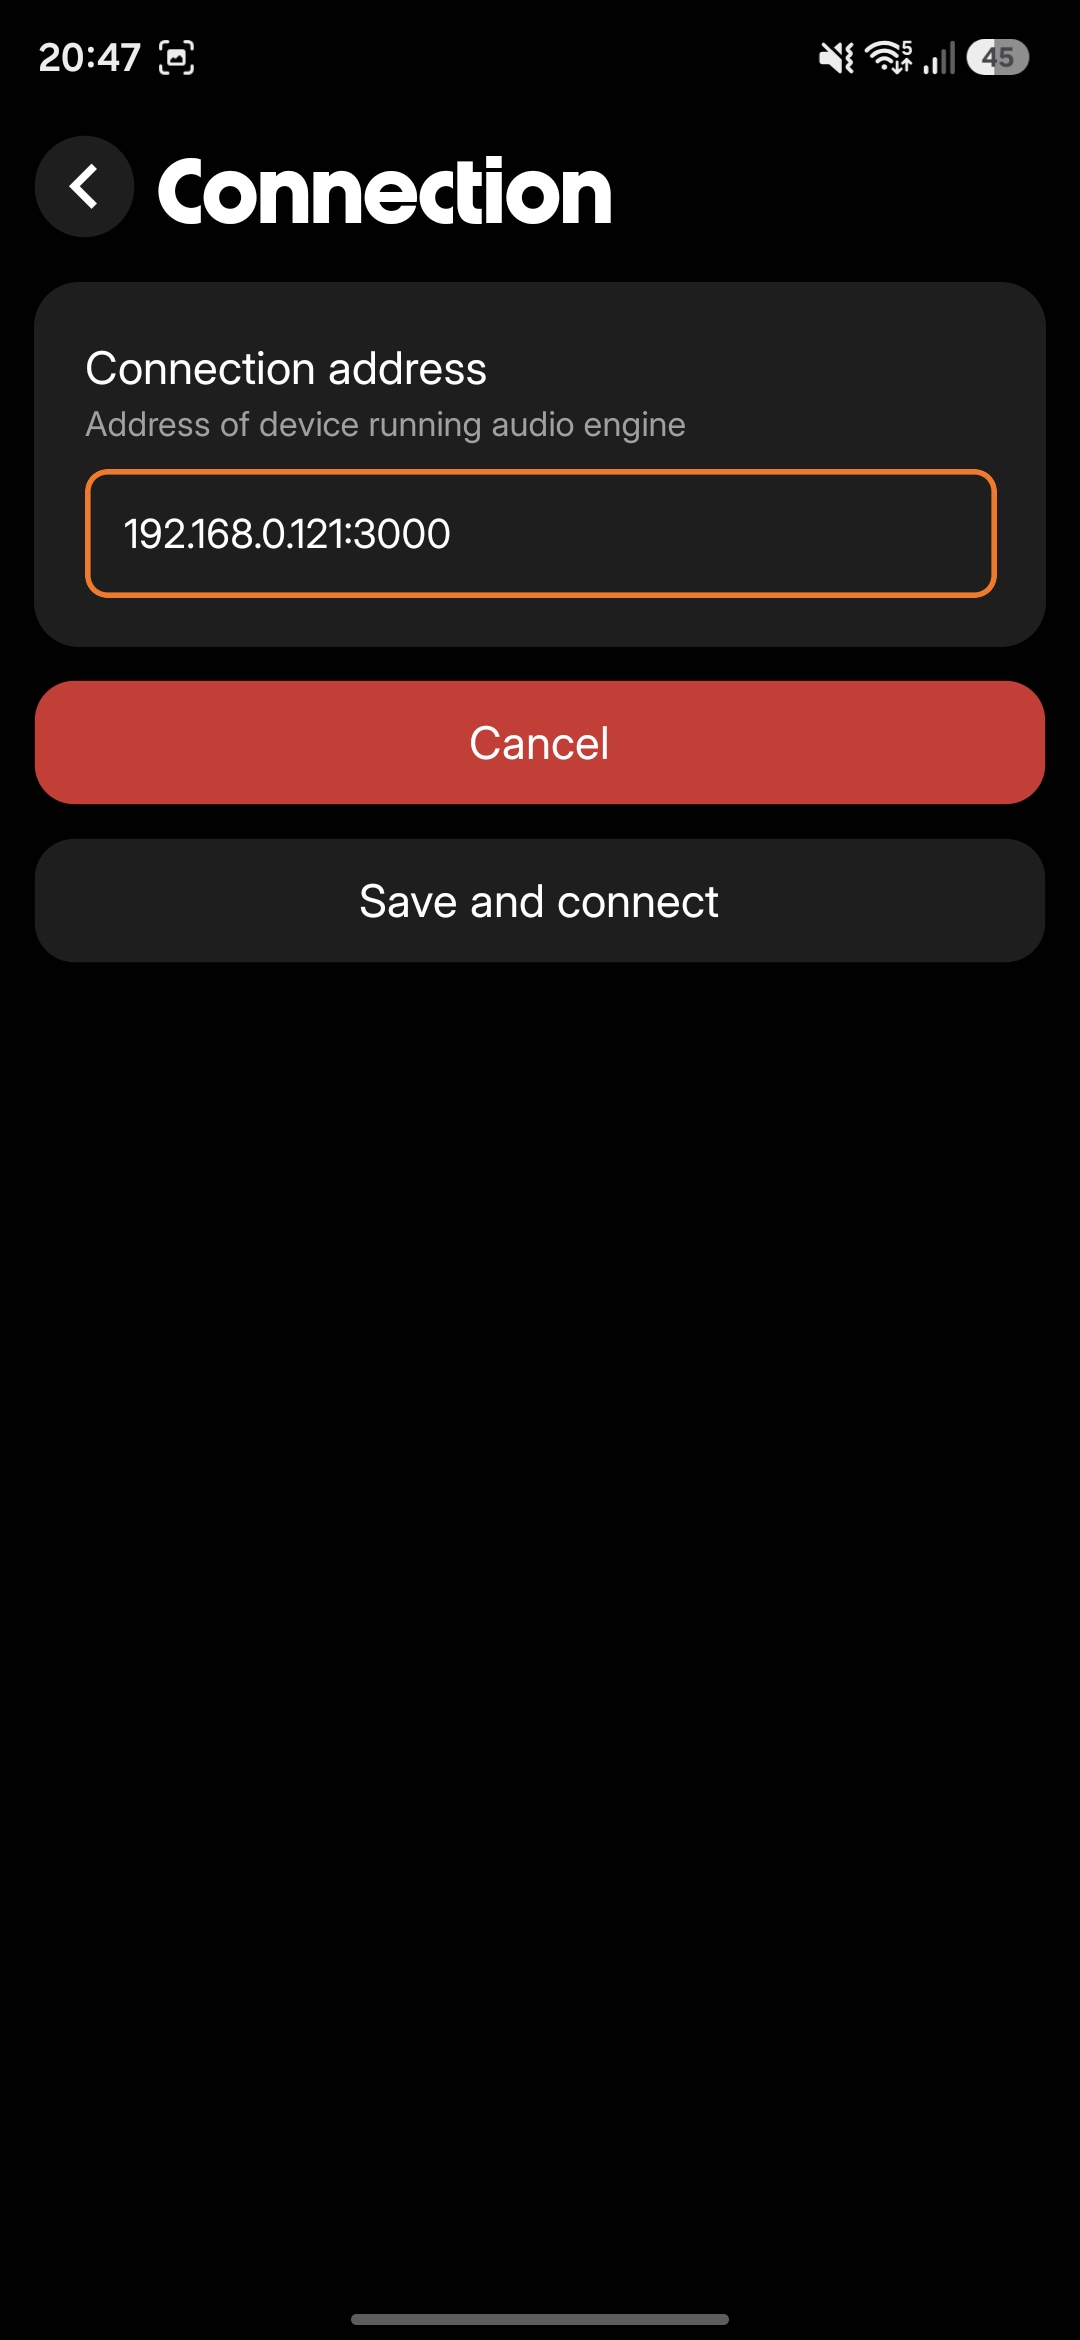
\includegraphics[width=\textwidth]{Screenshot_20260727_204756_Guitarian.jpg}
    \caption{Ekran ustawień - manualna konfiguracja połączenia[źródło własne]}
    \label{fig:settings_screen-connection_edit}
  \end{minipage}
\end{figure}

Za pomocą tego ekranu może zostać manualnie wprowadzony adres IP
serwera kontrolnego z uwzględnieniem jego portu. Po dotknięciu
przycisku zapisu, aplikacja spróbuje nawiązać połączenie z użyciem
podanego adresu. Gdy połączenie się uda, adres zostanie zapisany w
pamięci urządzenia, dzięki czemu może zostać użyty do zestawienia
połączenia przy ponownym uruchomieniu aplikacji.

\subsection{Konfiguracja opóźnień}
Kluczową opcją, która jest dostępna z poziomu ustawień aplikacji,
jest możliwość zarządzania wielkością bufora przetwarzanych próbek
dźwiękowych. Jak wspomniano we wcześniejszych sekcjach tego
dokumentu, wielkość ta ma bezpośrednie przełożenie na całkowite
opóźnienia. Użytkownik za pomocą rozwijanego menu może wybrać jedną
ze wspieranych wielkości bufora. Proces ten jest zobrazowany na
Rysunku \ref{fig:settings_screen-delay}.

\begin{figure}[H]
  \centering
  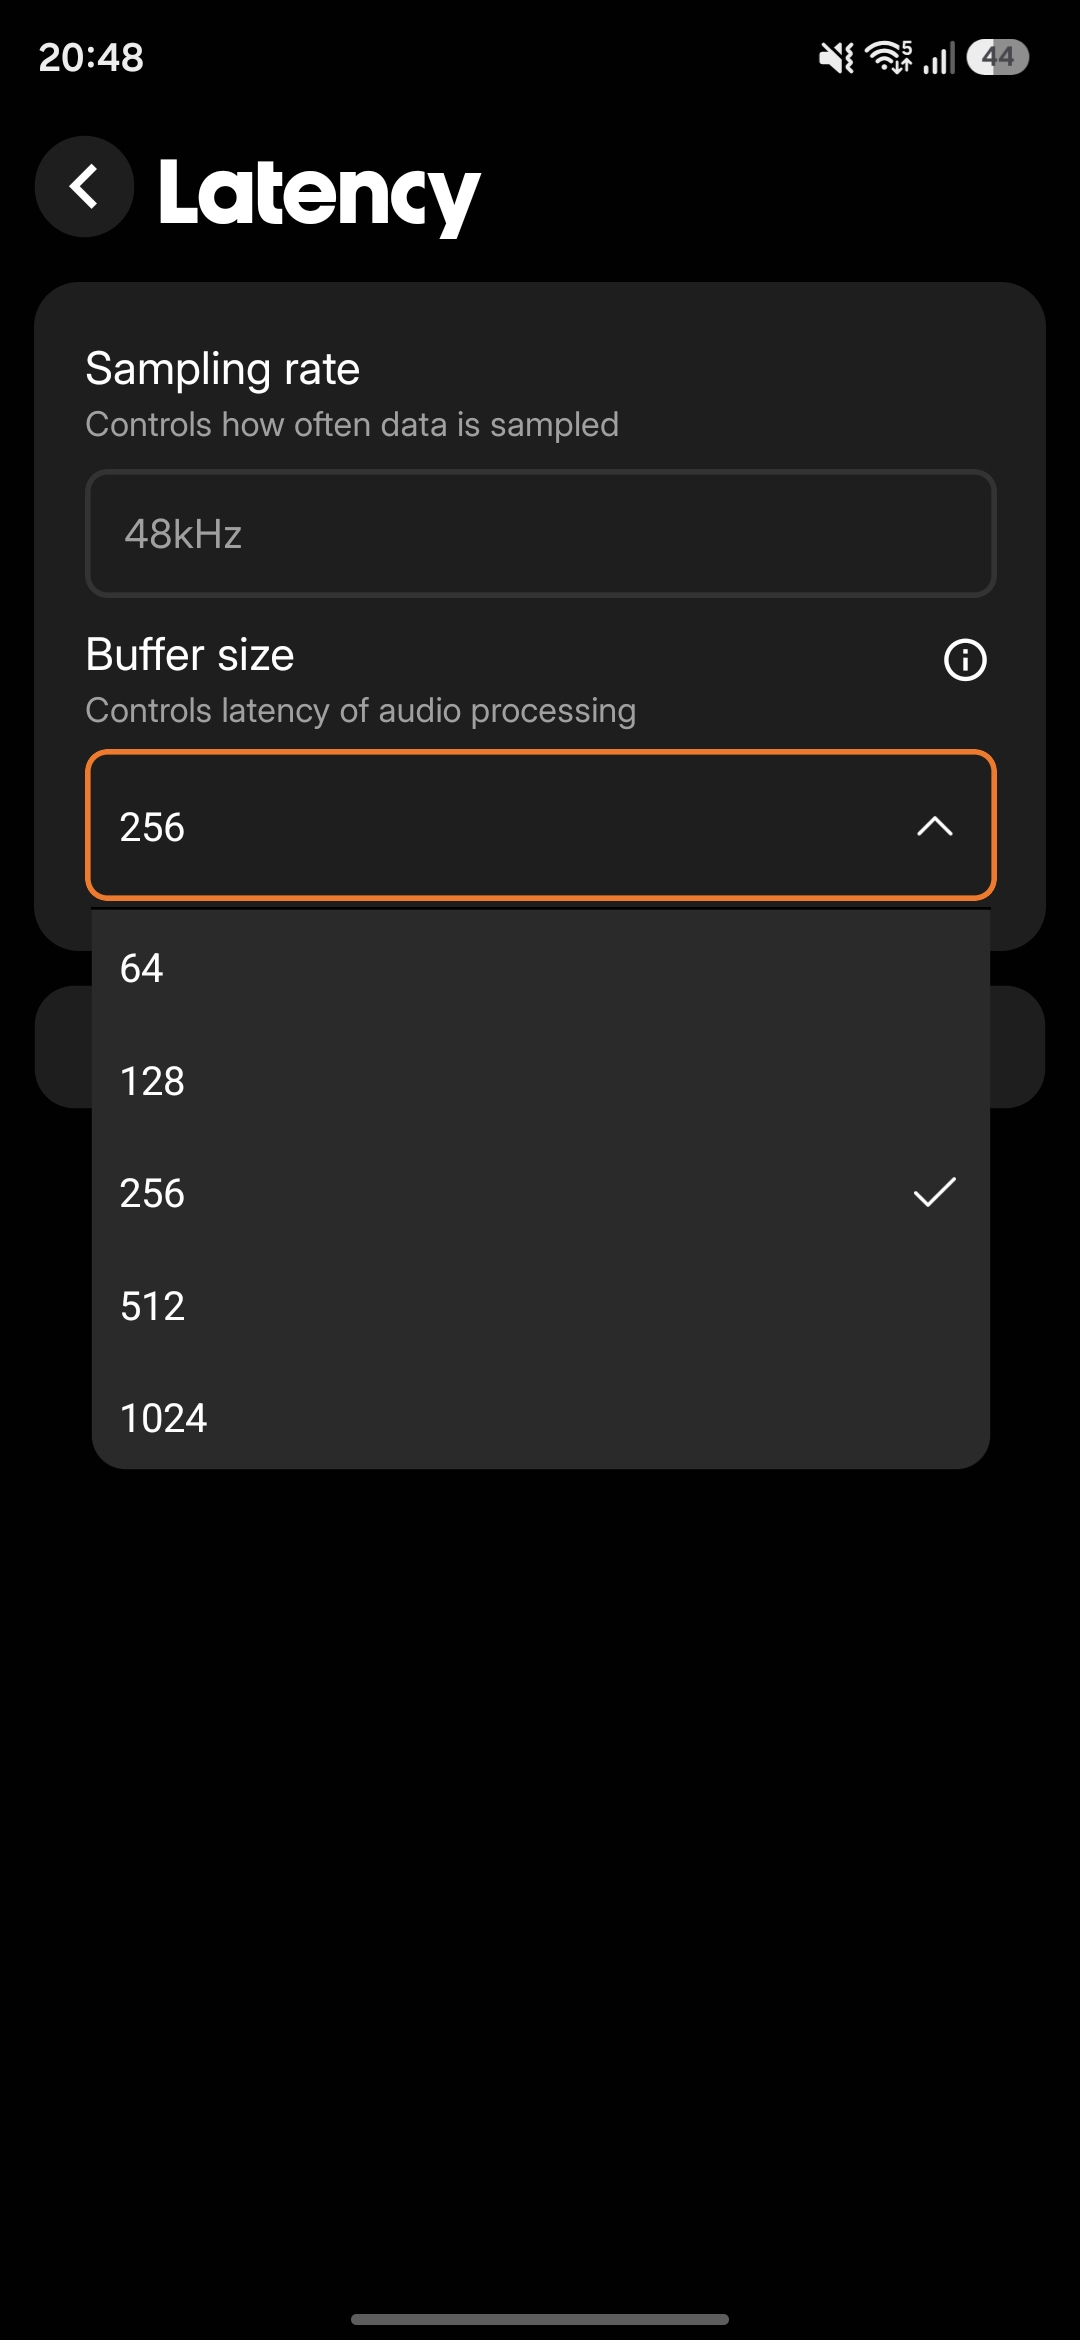
\includegraphics[width=0.5\textwidth]{Screenshot_20260727_204813_Guitarian.jpg}
  \caption{Ekran ustawień - konfiguracja opóźnień[źródło własne]}
  \label{fig:settings_screen-delay}
\end{figure}

Częstotliwość próbkowania widoczna na omawianym ekranie jest dostępna
tylko i wyłącznie w trybie do odczytu. Jest to świadoma decyzja,
która sprowadza się do tego, że w większości przypadków edycja tego
parametru niewiele wnosi do końcowej jakości dźwięku, a jej
niewłaściwa wartość może powodować spore problemy z końcową
wydajnością systemu, a także wpływać na prawidłową pracę niektórych
wtyczek audio. Zablokowana wartość 48kHz jest obecnie standardem,
który jest jednocześnie wspierany przez zdecydowaną większość interfejsów audio.

\chapter*{Podsumowanie}
\addcontentsline{toc}{chapter}{Podsumowanie}
W ramach niniejszej pracy zaprojektowano i zaimplementowano w pełni
funkcjonalne oraz użyteczne rozwiązanie dedykowane gitarzystom.
Nadrzędnym celem projektu było stworzenie środowiska, które z
powodzeniem łączy zaawansowane możliwości cyfrowego przetwarzania
sygnału z maksymalną przystępnością i prostotą obsługi. Zaproponowany
interfejs użytkownika aplikacji mobilnej charakteryzuje się wysoką
intuicyjnością i wygodą użytkowania.

Zrealizowany system dostarcza kompletny zestaw funkcjonalności, które
są konieczne w obcowaniu z cyfrowymi efektami gitarowymi. Użytkownik
otrzymał do dyspozycji mechanizmy dodawania, usuwania oraz
rekonfiguracji kolejności wtyczek w torze sygnałowym. System pozwala
na płynną regulację parametrów wtyczek i możliwość oceny dokonanych
zmian z bardzo małymi opóźnieniami. System posiada również szereg
udogodnień takich jak możliwość tworzenia i zarządzania własnymi
profilami brzmieniowymi czy łatwą konfigurację parametrów
środowiskowych z poziomu smartfona. Z inżynieryjnego punktu widzenia
projekt udowadnia skuteczność przyjętych założeń architektonicznych.
System charakteryzuje się wysoce wydajnym i stabilnym przetwarzaniem
dźwięku oraz błyskawiczną, asynchroniczną komunikacją sieciową
pomiędzy silnikiem audio a aplikacją kliencką. Co istotne, elastyczna
i modularna architektura systemu pozwala na łatwą rozbudowę jego
komponentów, a wydzielenie warstwy interfejsu graficznego do
aplikacji mobilnej jest świetnym rozwiązaniem dla niewielkich
komputerów jednopłytkowych, jak np. Raspberry Pi.

Choć zaprezentowany system jest rozwiązaniem kompletnym, to jego
architektura stwarza szerokie perspektywy dla dalszego rozwoju.
Bezpośrednim kierunkiem rozbudowy powinno być zaimplementowanie
wsparcia dla dodatkowych, powszechnie stosowanych standardów wtyczek
(np. VST3, CLAP). Niezwykle atrakcyjnym krokiem byłaby również
integracja z technologią NAM (ang. \textit{Neural Amp Modeler}),
umożliwiająca wykorzystanie wtyczek opartych na zaawansowanych
modelach uczenia maszynowego do dokładnej symulacji analogowych
wzmacniaczy i efektów. Ponadto użytecznym rozszerzeniem z perspektywy
muzyka byłaby integracja tunera gitarowego.

\printbibliography[heading=bibintoc,title={Bibliografia}]

\end{document}
